\documentclass[a4paper,11pt]{article}
\usepackage[a4paper,margin=2.5cm]{geometry}
\usepackage[T1]{fontenc}
\usepackage[utf8]{inputenc}
\usepackage[slovak]{babel}
\usepackage{textcomp}
\usepackage{amsmath,amssymb}
\usepackage{graphicx}
\usepackage{array,booktabs,longtable}
\usepackage{microtype}
\graphicspath{{img/}{dokumentacia/img/}}
\setcounter{secnumdepth}{3}
\renewcommand{\thesection}{\arabic{section}.}
\renewcommand{\thesubsection}{\arabic{section}.\arabic{subsection}.}
\renewcommand{\thesubsubsection}{\arabic{section}.\arabic{subsection}.\arabic{subsubsection}.}
\pagestyle{plain}
\title{SUNS: zadanie 2}
\author{Samuel Bagin}
\date{}
\emergencystretch=2em
\providecommand{\tightlist}{\setlength{\itemsep}{0pt}\setlength{\parskip}{0pt}}
\DeclareUnicodeCharacter{00B3}{\textsuperscript{3}}
\DeclareUnicodeCharacter{00B2}{\textsuperscript{2}}
\DeclareUnicodeCharacter{2212}{\ensuremath{-}}
\DeclareUnicodeCharacter{2192}{\ensuremath{\rightarrow}}
\DeclareUnicodeCharacter{00B1}{\ensuremath{\pm}}
\begin{document}
\maketitle
% main.ipynb: bunka 0
\section{Úprava dát}

% main.ipynb: bunka 0¸
Predikcia priemernej hodinovej koncentrácie CO pomocou regresných modelov. Výstup \texttt{co} je v mg/m³. Do vstupov modelov nevstupuje.

Načítal som \textbf{9,507 riadkov a 14 stĺpcov}. Merania pokrývajú obdobie \textbf{2004-03-10 až 2005-04-04}.

% main.ipynb: bunka 6
\subsection{Kvalita dát}

% main.ipynb: bunka 6
Odstraňujem riadky s NA, a nerobím imputáciu. Duplicity skontrolujem ešte pred rozdelením, aby rovnaké meranie neskončilo v tréningu aj teste. Pri dátume overím parsovanie a súlad s mesiacom a dňom v týždni.

% main.ipynb: bunka 8
Dataset obsahuje \textbf{150 duplicít}. Cieľový stlpec chýba v \textbf{1716 riadkoch}.

\begin{center}
\noindent
\begin{minipage}[c]{0.32\linewidth}
\centering
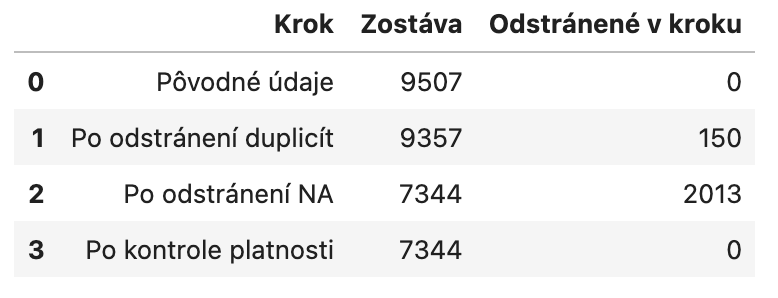
\includegraphics[width=\linewidth,keepaspectratio]{data_cistenie_tabulka.png}
\end{minipage}\hfill%
\begin{minipage}[c]{0.65\linewidth}
\centering
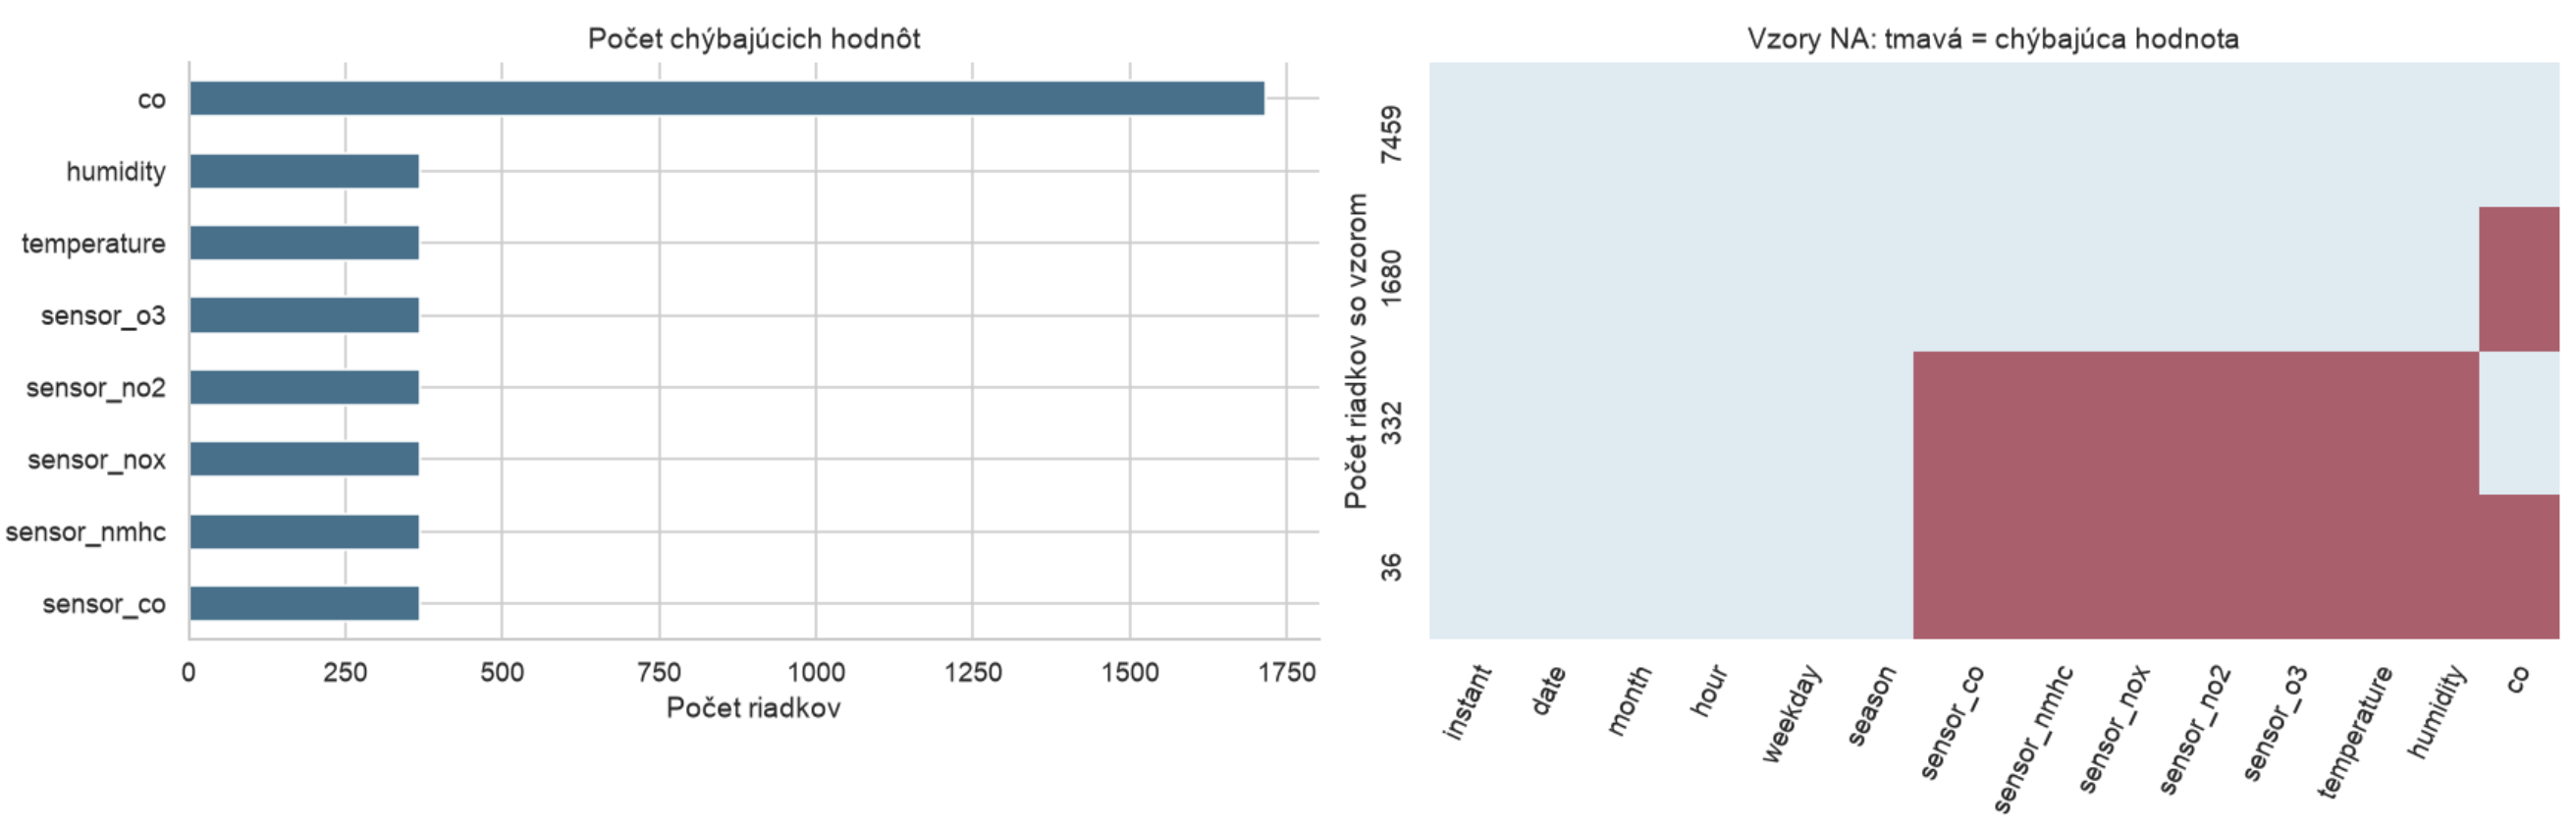
\includegraphics[width=\linewidth,keepaspectratio]{data_chybajuce_hodnoty_graf.png}
\end{minipage}
\end{center}

% main.ipynb: bunka 10
Po čistení zostalo \textbf{7,344 úplných a platných meraní} (77.2\% pôvodných riadkov). Teploty nad približných 40 °C automaticky nemažem: stále môžu byť reálnym meraním. Štatistické outliery odstránim až z tréningových dát pomocou hraníc naučených výhradne na danom tréningu.

\begin{center}
\noindent
\begin{minipage}[c]{0.28\linewidth}
\centering
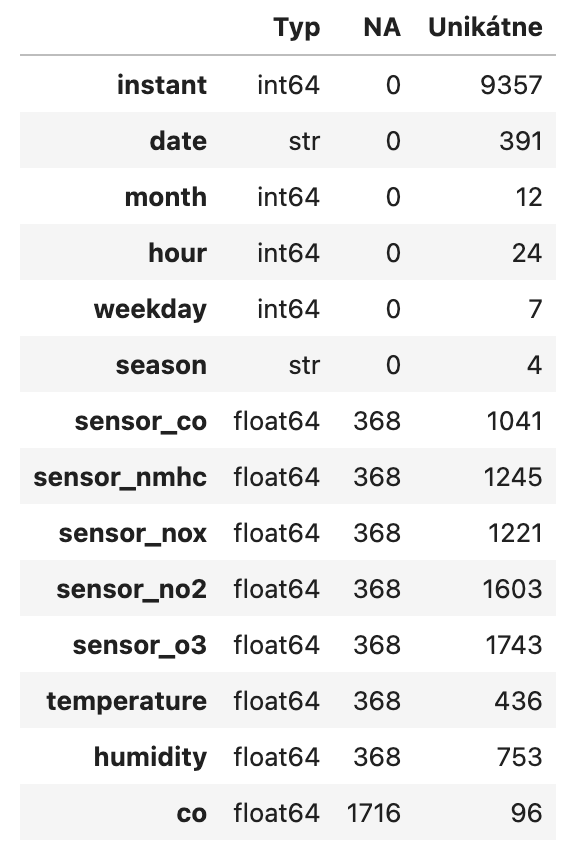
\includegraphics[width=\linewidth,keepaspectratio]{data_kvalita_stlpcov_tabulka.png}
\end{minipage}\hfill%
\begin{minipage}[c]{0.69\linewidth}
\centering
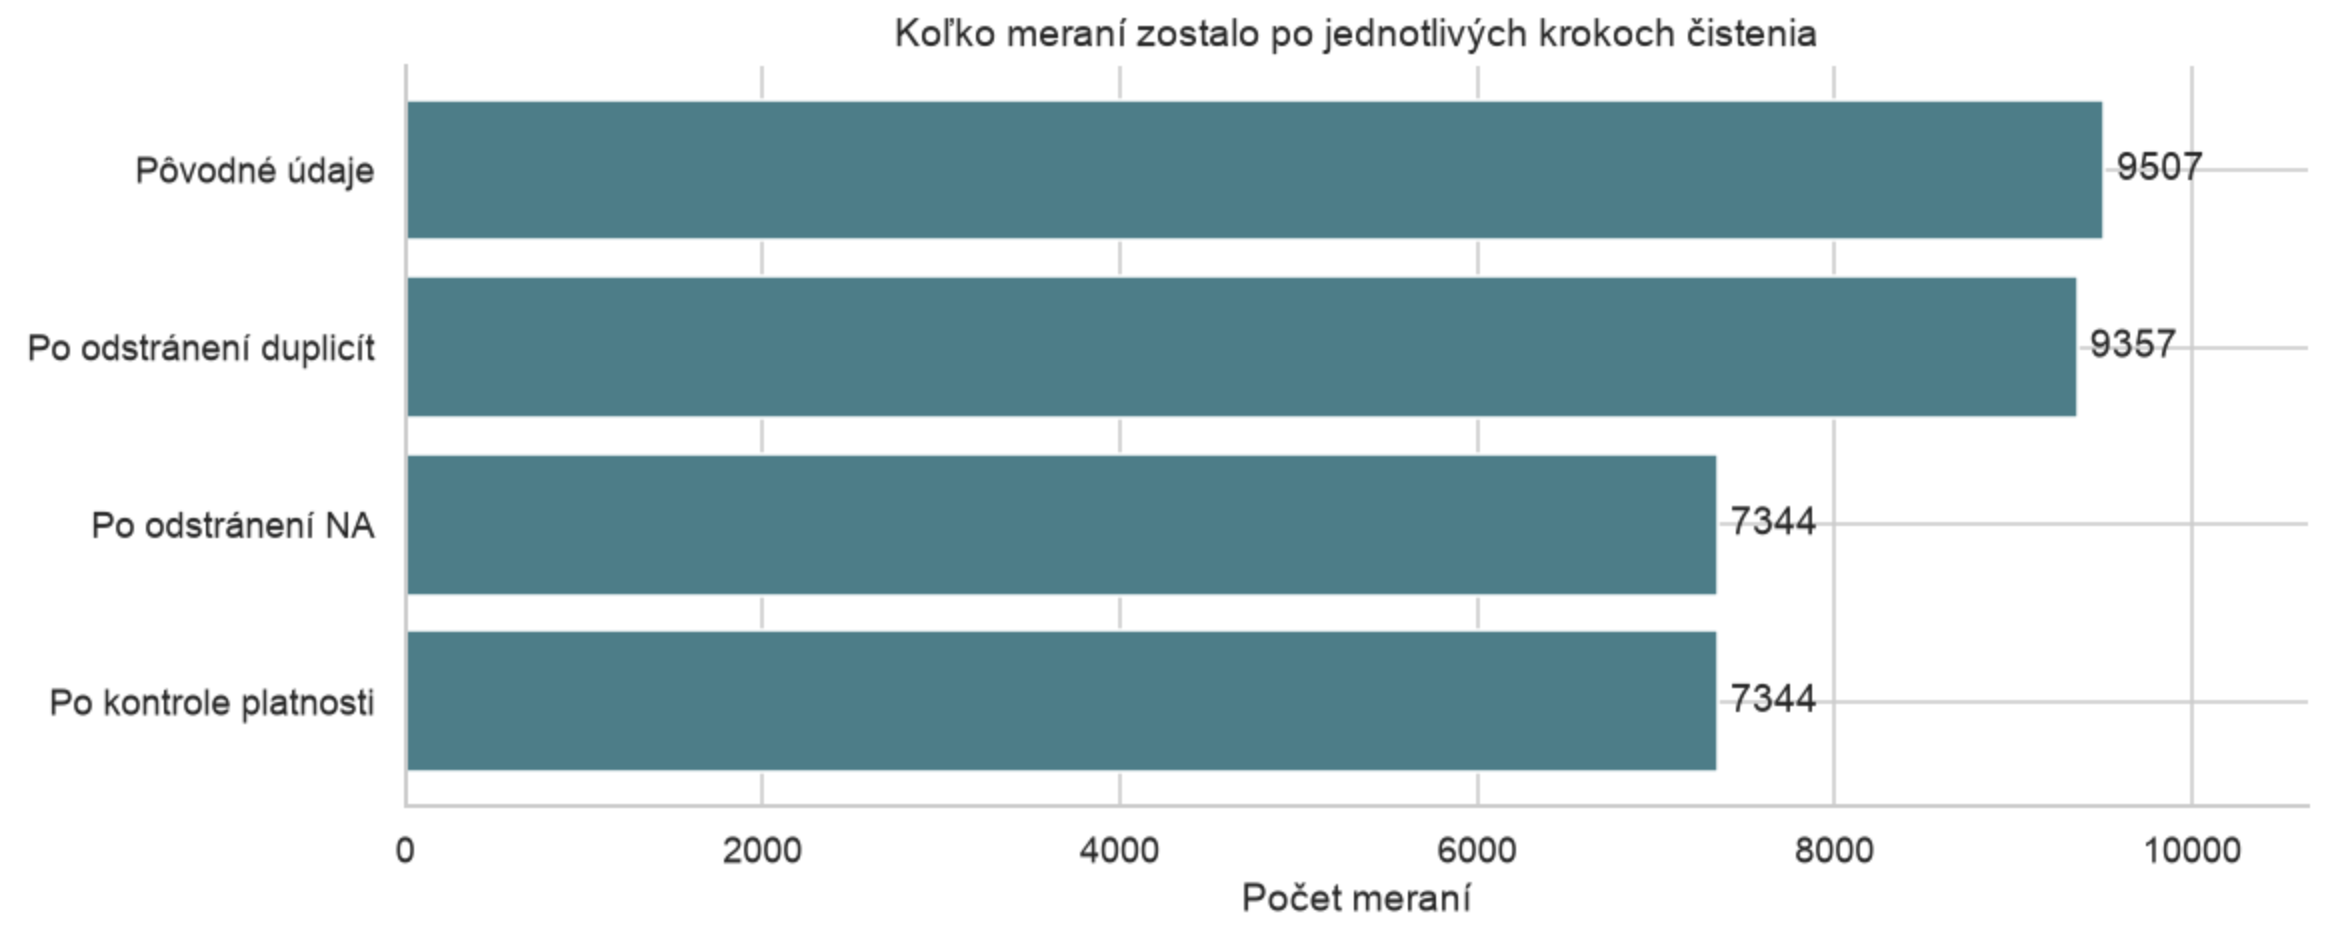
\includegraphics[width=\linewidth,keepaspectratio]{data_cistenie_graf.png}
\end{minipage}
\end{center}

Tabuľka kvality uvádza stav po odstránení duplicít, pred odstránením NA.

\subsubsection{Ukážka dát a opisná štatistika}

Ukážka riadkov a opisná štatistika zachytávajú pôvodné načítané údaje pred čistením.

\begin{center}
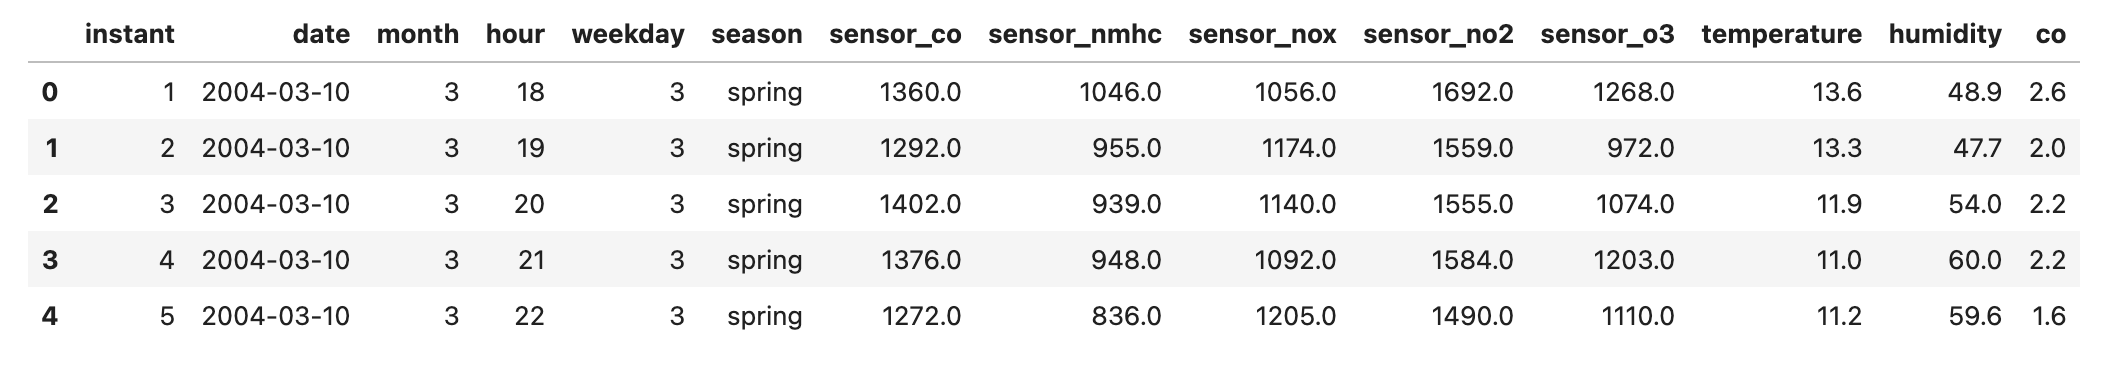
\includegraphics[width=\linewidth,keepaspectratio]{data_prve_riadky_tabulka.png}
\end{center}

\begin{center}
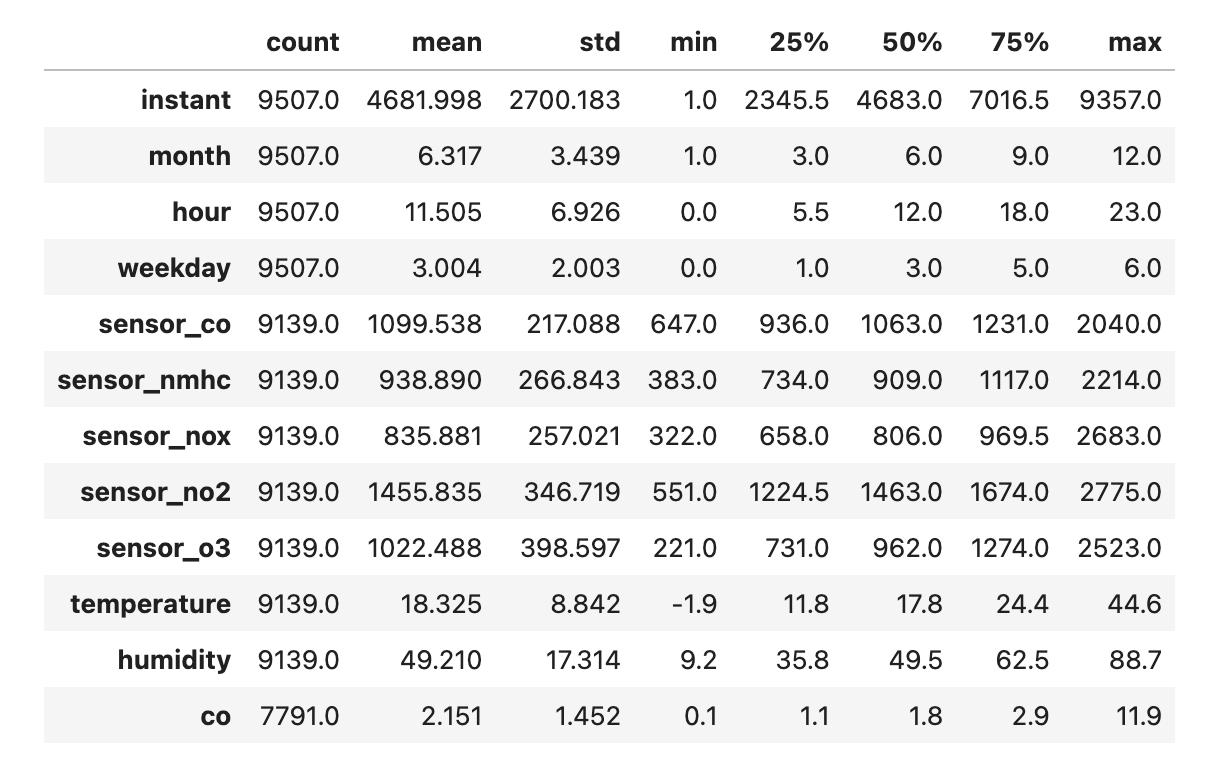
\includegraphics[width=0.52\linewidth,keepaspectratio]{data_popisna_statistika_tabulka.png}
\end{center}

% main.ipynb: bunka 13
\section{EDA -- bonus}

% main.ipynb: bunka 14
\subsection{Rozdelenia senzorov a koncentrácie}

\begin{center}
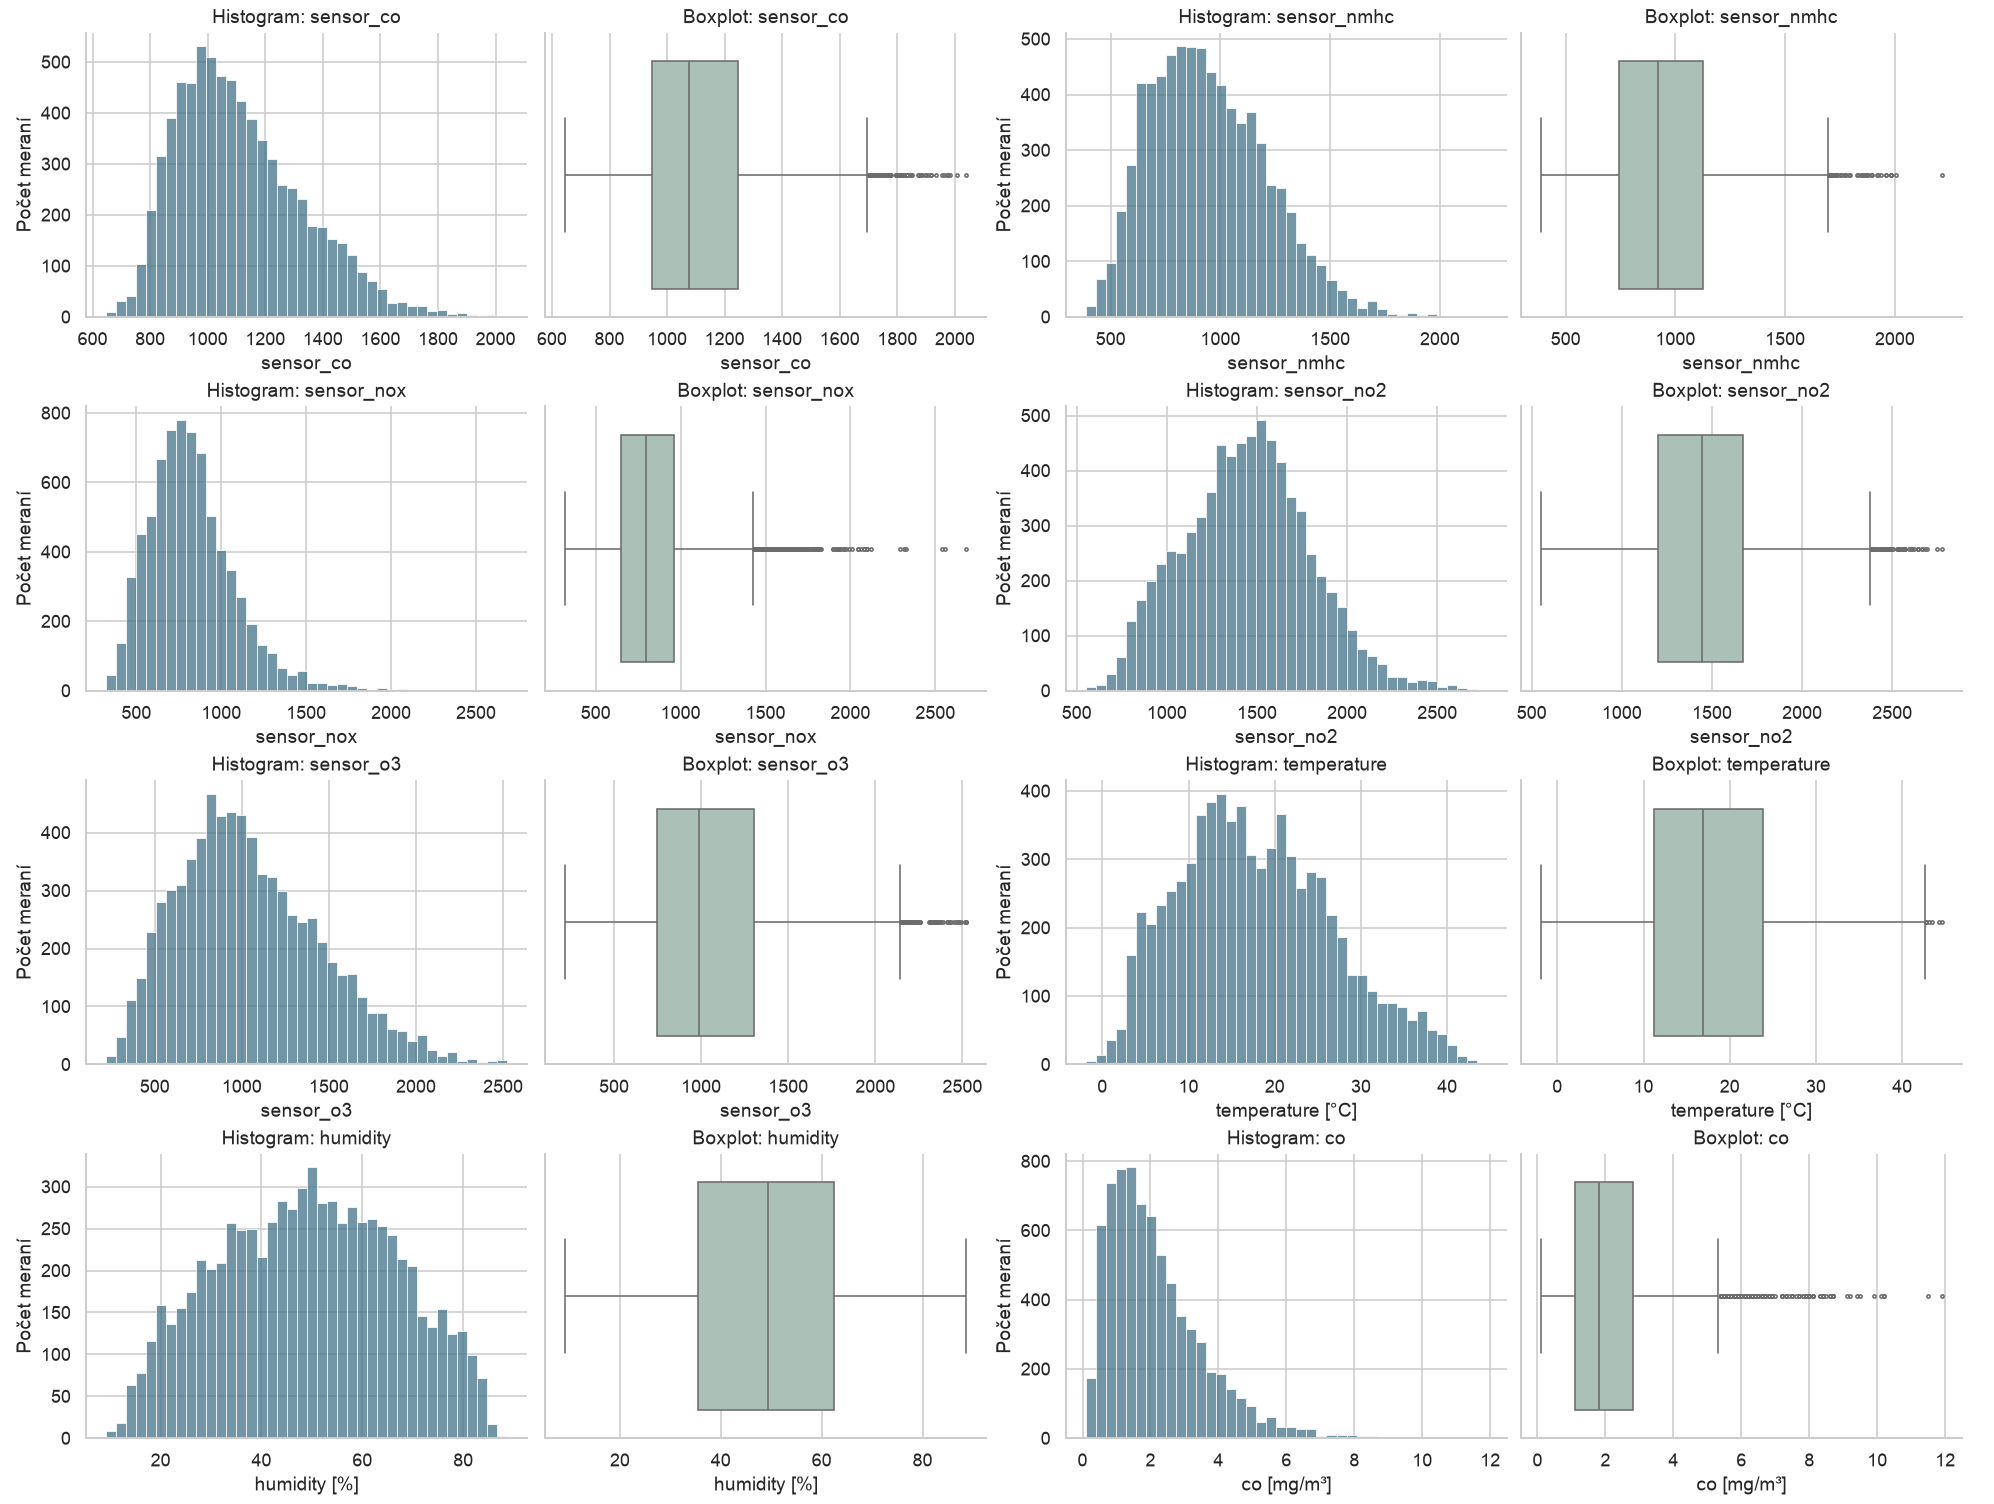
\includegraphics[width=0.72\linewidth,keepaspectratio,height=0.40\textheight]{eda_histogramy_a_boxploty_graf.png}
\end{center}

% main.ipynb: bunka 16
CO má medián \textbf{1.80 \(\mathrm{mg}/\mathrm{m}^3\)}, priemer 2.13 \(\mathrm{mg}/\mathrm{m}^3\) a výberovú šikmosť \textbf{1.36}. Dlhší pravý chvost znamená menej časté vysoké koncentrácie. MSE tieto veľké chyby silno penalizuje. Senzor NOx dosahuje maximum 2683. Odľahlosť v grafe sama nepreukazuje poruchu.

% main.ipynb: bunka 17
\subsection{Súvislosti a časový priebeh}

\begin{center}
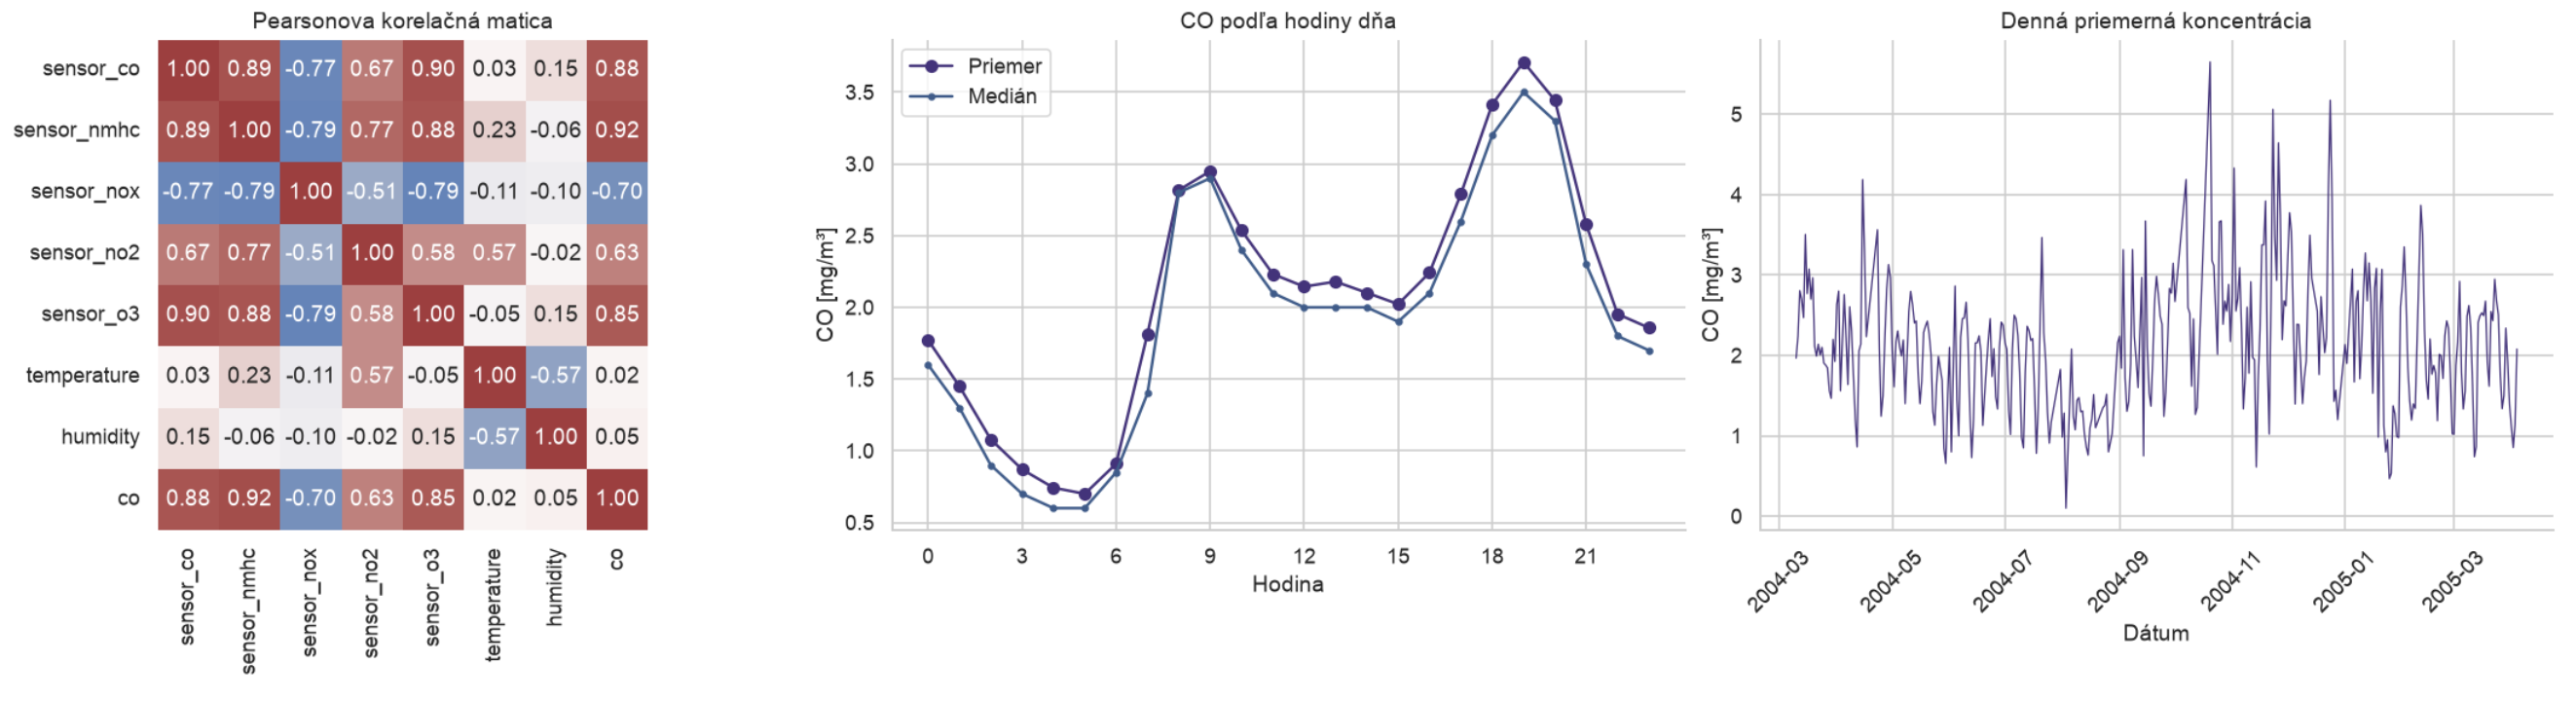
\includegraphics[width=\linewidth,keepaspectratio]{eda_korelacie_a_casovy_priebeh_graf.png}
\end{center}

% main.ipynb: bunka 19
Najsilnejšiu absolútnu Pearsonovu koreláciu s CO má \textbf{sensor\_nmhc}, \(r = 0.92\), a \textbf{sensor\_o3} voči \textbf{sensor\_co} \(r = 0.90\). Najvyšší hodinový priemer je o \textbf{19:00} (3.71 \(\mathrm{mg}/\mathrm{m}^3\)), najnižší o 5:00 (0.70 \(\mathrm{mg}/\mathrm{m}^3\)). Rozdiely sú zlučiteľné s denným cyklom emisií, ale bez údajov o doprave a počasí z grafu nemožno potvrdiť jeho príčinu. Denný priebeh ukazuje aj časovú závislosť, ktorú obyčajné náhodné rozdelenie úplne neodstraňuje.

\subsection{Hodinový priebeh CO v pracovných dňoch a cez víkend}

\begin{center}
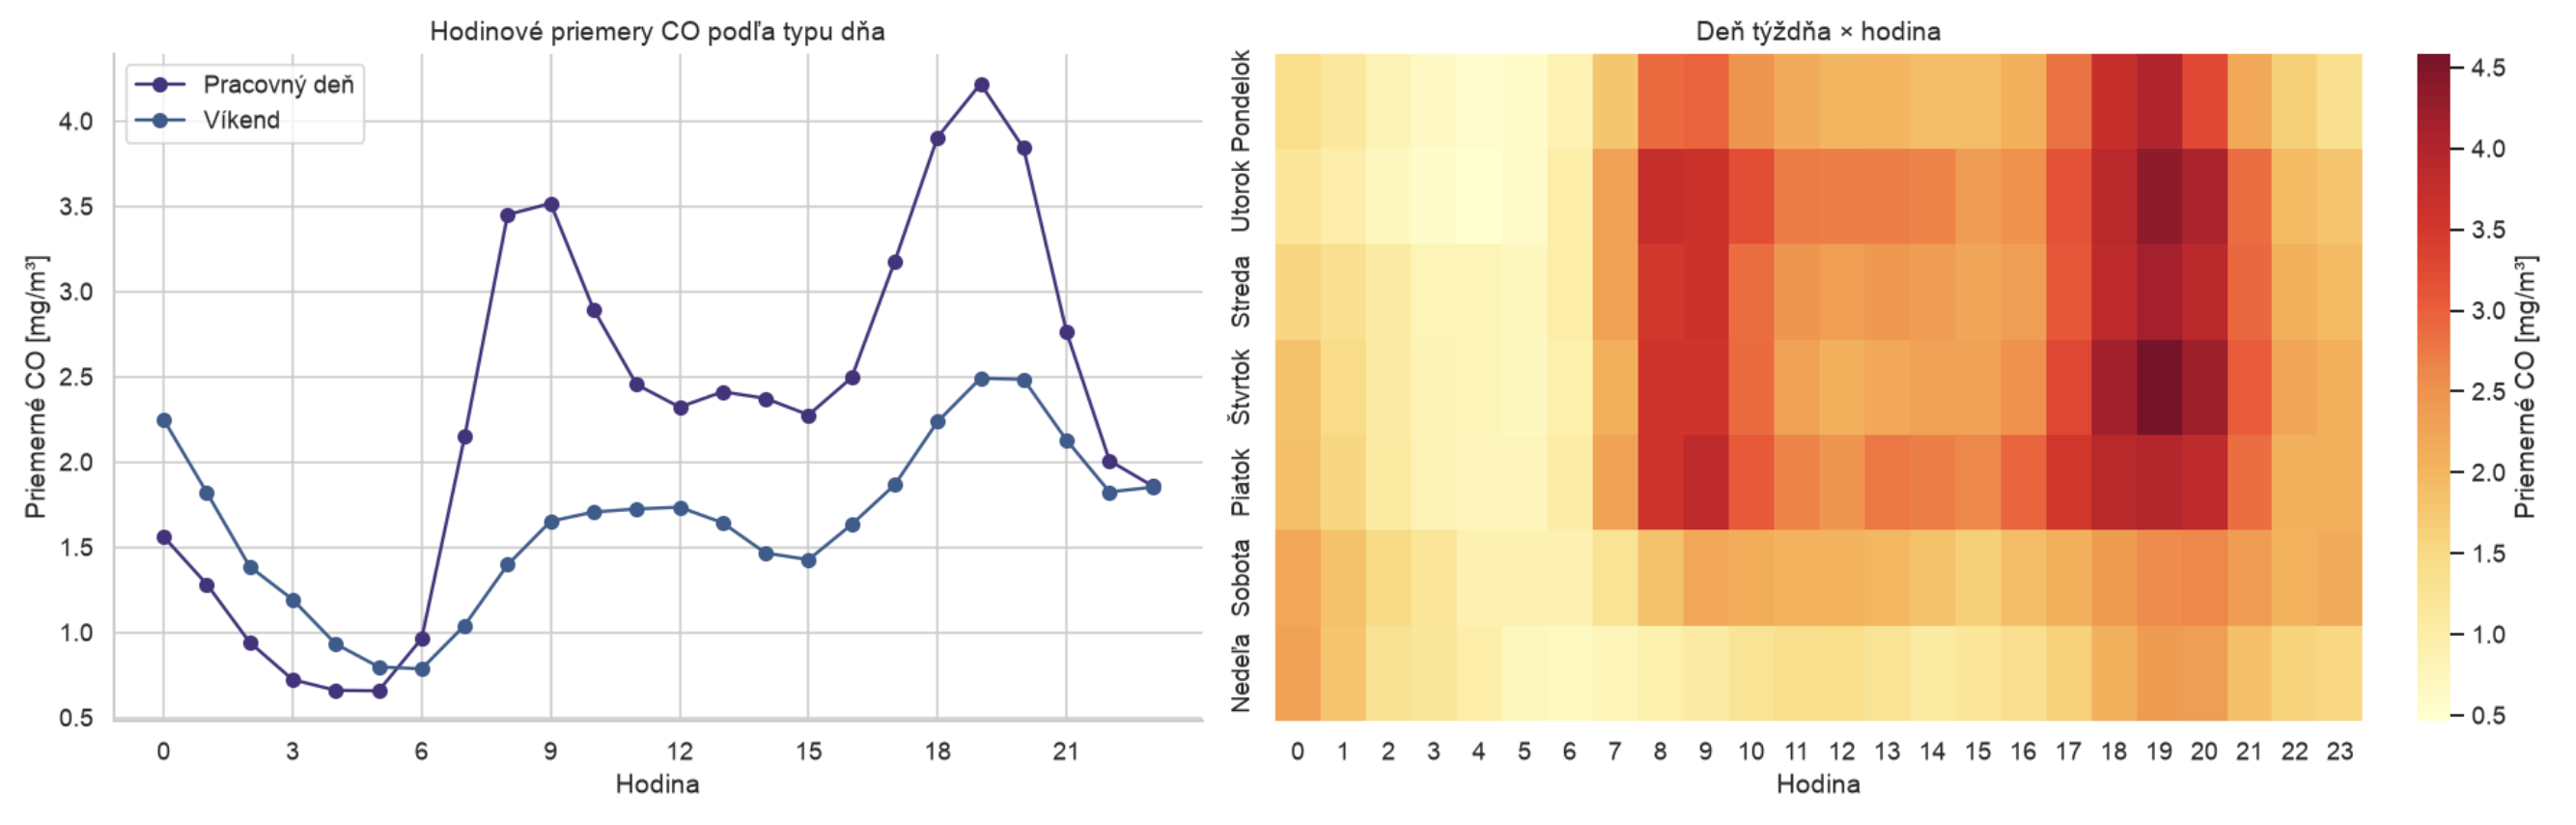
\includegraphics[width=\linewidth,keepaspectratio]{eda_co_pracovne_dni_a_vikend_graf.png}
\end{center}

% main.ipynb: bunka 22
Pracovné dni majú priemerné CO \textbf{2.333 mg/m³}, víkend \textbf{1.658 mg/m³}. Najvyšší hodinový priemer nastáva v pracovných dňoch o \textbf{19:00}, cez víkend o \textbf{19:00}. Priemery sú ovplyvnené aj zastúpením ročných období a počasia. Samy nepotvrdzujú príčinný vplyv dopravy.

\subsection{Teplota, vlhkosť a koncentrácia CO}

\begin{center}
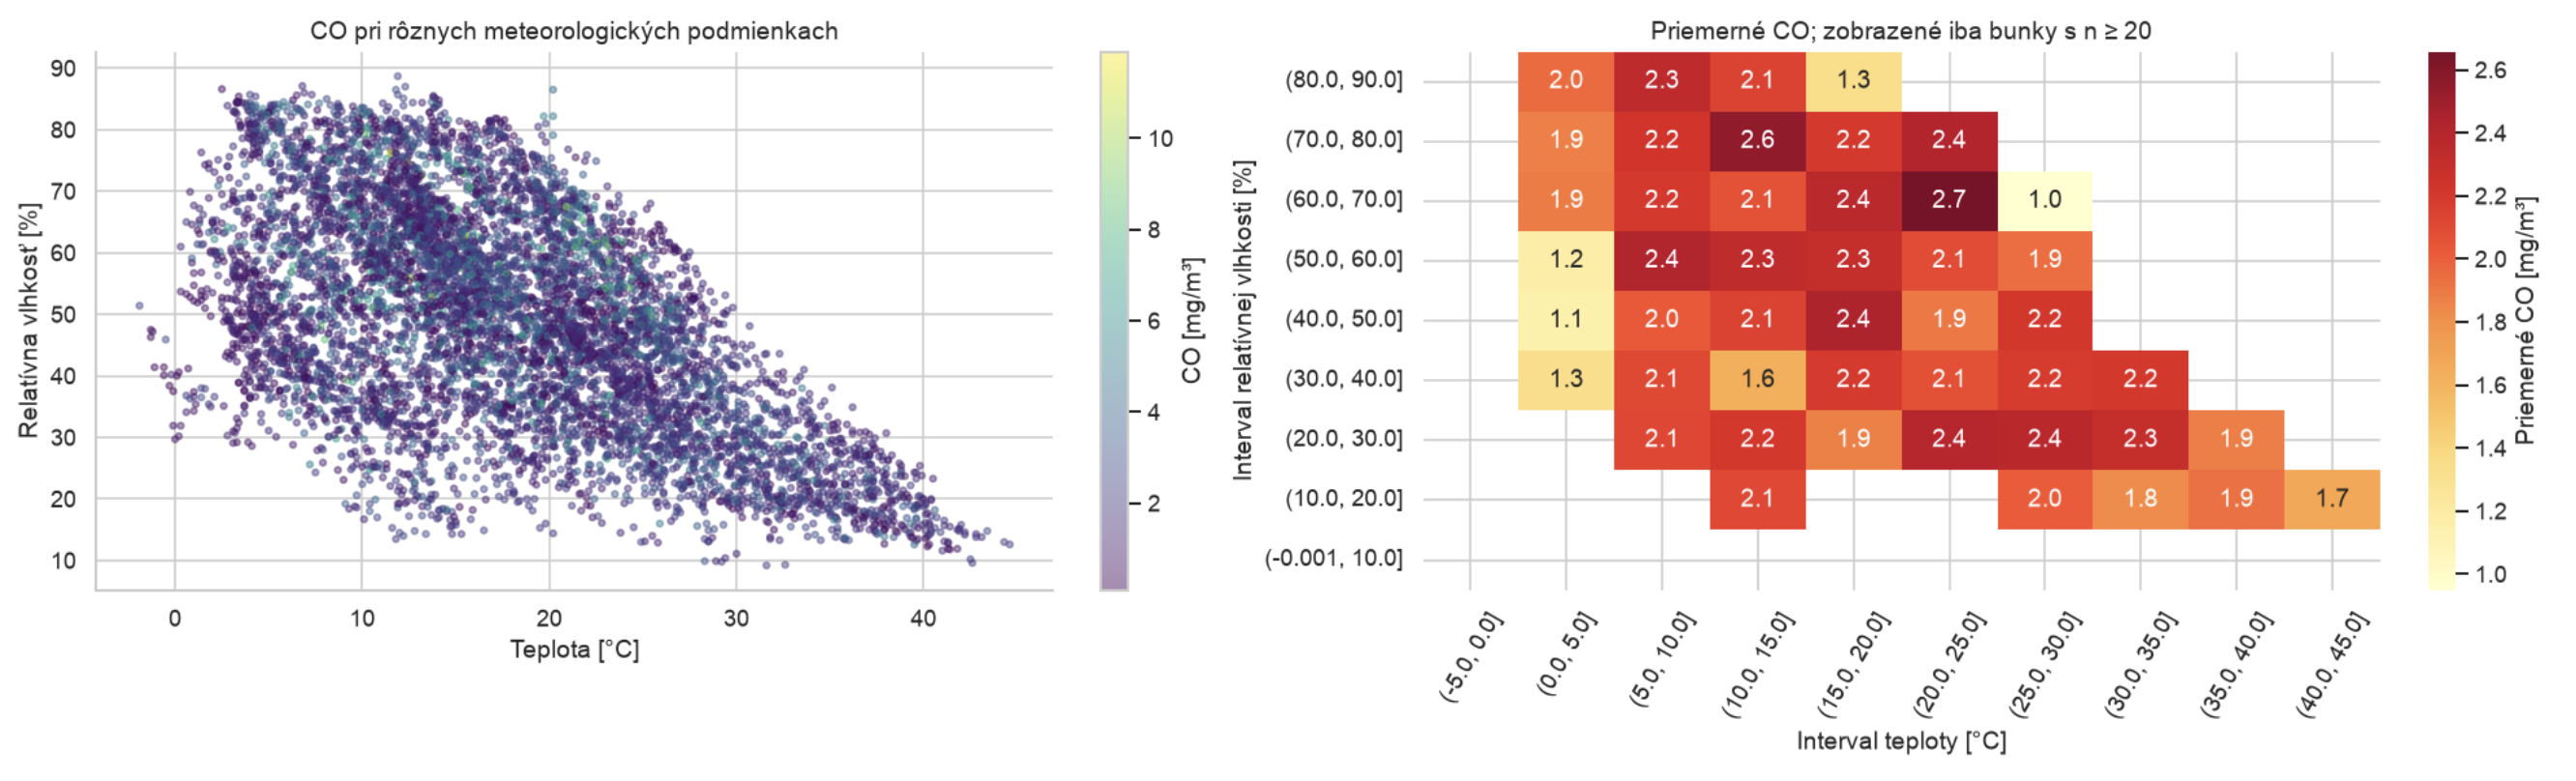
\includegraphics[width=\linewidth,keepaspectratio]{eda_co_teplota_a_vlhkost_graf.png}
\end{center}

% main.ipynb: bunka 25
Spearmanova korelácia CO s teplotou je \textbf{0.069}, s vlhkosťou \textbf{-0.006}. Zo zobrazených buniek s aspoň 20 meraniami má najvyššie priemerné CO kombinácia teploty \textbf{(20.0, 25.0{]} °C} a vlhkosti \textbf{(60.0, 70.0{]} \%} (\textbf{2.658 mg/m³}), najnižší priemer je \textbf{0.950 mg/m³}. Agregovaný graf ukazuje spoločný vzťah dvoch premenných, ale nenahrádza kontrolu sezónnosti ani dôkaz príčiny. Biele bunky nemajú dosť meraní na zobrazenie.

\begin{center}
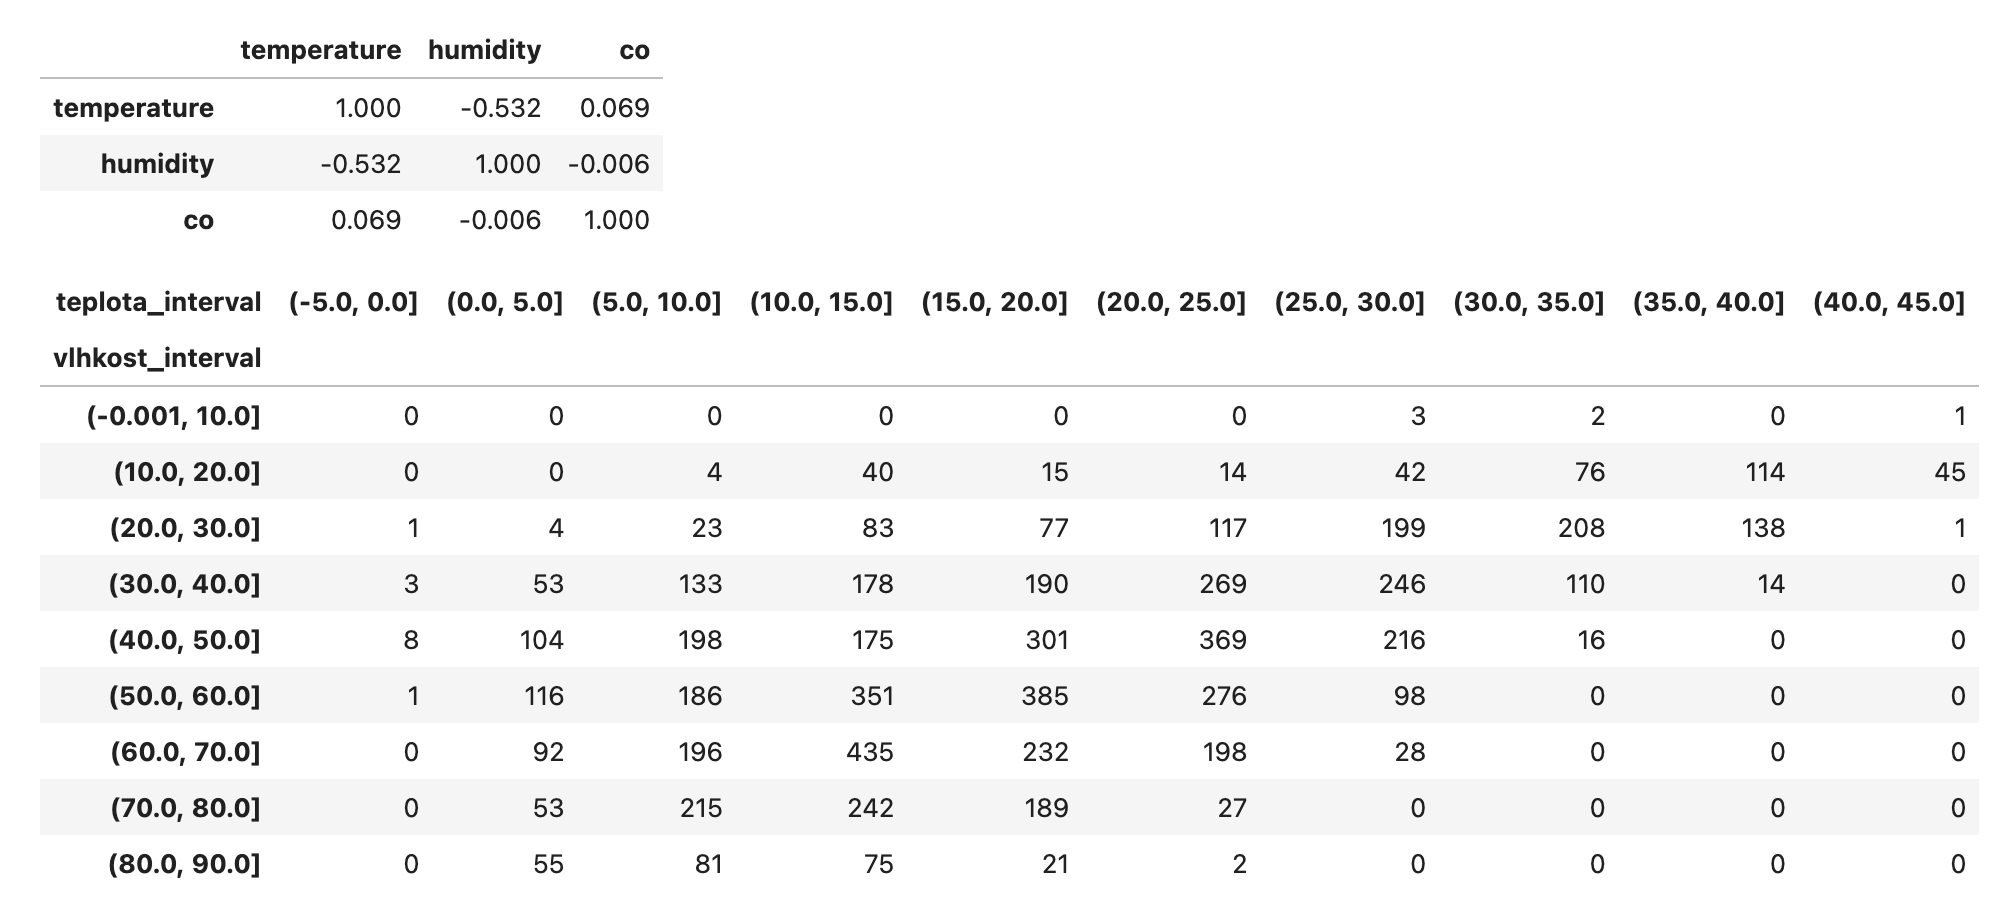
\includegraphics[width=0.7\linewidth,keepaspectratio]{eda_korelacie_a_pocty_meteo_tabulka.png}
\end{center}

% main.ipynb: bunka 26
\section{Rozdelenie dát}

% main.ipynb: bunka 26
Použijem jedno rozdelenie \textbf{80 \% tréning / 20 \% test}. Tréning zahŕňa aj vnútorné CV foldy, preto samostatnú vonkajšiu validačnú množinu nepotrebujem. Seed 2026 je stanovený pred týmto experimentom. \texttt{instant} a \texttt{date} sa do modelov nedostanú. Rovnaké testovacie riadky zachovám aj pri redukcii príznakov a zhlukovaní.

% main.ipynb: bunka 28
Tréning obsahuje \textbf{5875} a test \textbf{1469} meraní. Rozdelenie je náhodné bez stratifikácie regresného cieľa.

\begin{center}
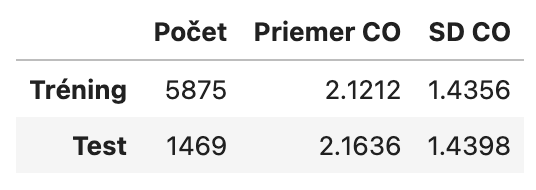
\includegraphics[width=0.39\linewidth,keepaspectratio]{data_rozdelenie_trening_test_tabulka.png}\hfill
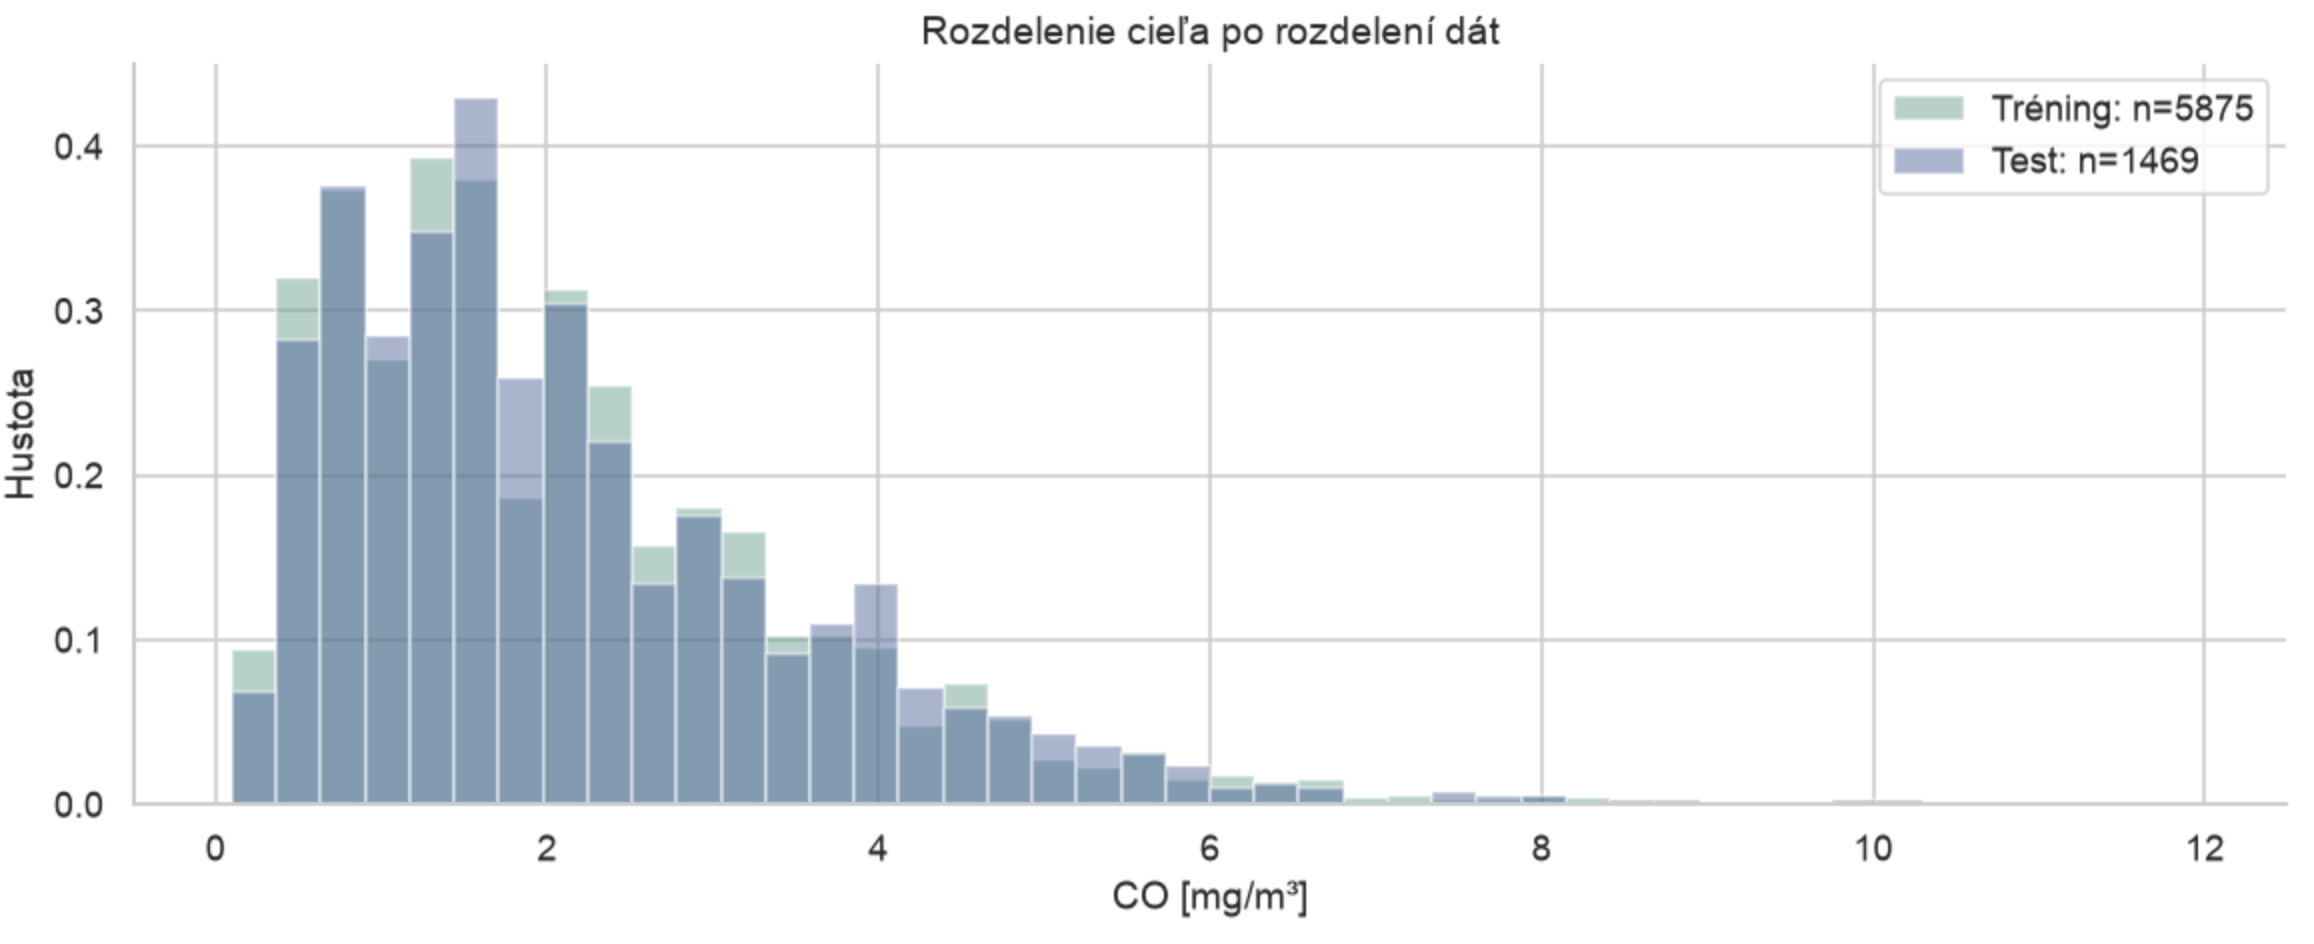
\includegraphics[width=0.58\linewidth,keepaspectratio]{data_rozdelenie_trening_test_graf.png}
\end{center}

% main.ipynb: bunka 31
\subsection{Kódovanie a normalizácia}

\subsubsection{Cyklické kalendárne premenné}

Mesiac, hodinu a deň v týždni prevediem na sínus a kosínus. Susedné hodnoty 23 a 0 hodín tak zostanú blízko aj v kódovaní. Sezóna má iba štyri kategórie, preto použijem one-hot kódovanie. Dátum nepridáva stovky stĺpcov. Po kódovaní štandardizujem \textbf{všetky vstupy}, vrátane one-hot stĺpcov, aby PCA a vzdialenostné modely neovládla pôvodná mierka senzorov. Cieľ \texttt{co} nemením.

\[
\begin{aligned}
\mathrm{sin}_t &= \sin\left(\frac{2\pi t}{T}\right), \quad \mathrm{cos}_t = \cos\left(\frac{2\pi t}{T}\right) \\
z &= \frac{x - \mu_{\text{tréning}}}{\sigma_{\text{tréning}}}
\end{aligned}
\]

Kódovaním vzniká \textbf{17 vstupov}, 10 nových stĺpcov, ktoré nahradili 4 pôvodné.

\begin{itemize}
\tightlist
\item
  month (cyclic): \texttt{month\_\allowbreak{}sin}, \texttt{month\_\allowbreak{}cos}
\item
  hour (cyclic): \texttt{hour\_\allowbreak{}sin}, \texttt{hour\_\allowbreak{}cos}
\item
  weekday (cyclic): \texttt{weekday\_\allowbreak{}sin}, \texttt{weekday\_\allowbreak{}cos}
\item
  season (one-hot): \texttt{season\_\allowbreak{}autumn}, \texttt{season\_\allowbreak{}spring}, \texttt{season\_\allowbreak{}summer}, \texttt{season\_\allowbreak{}winter}
\end{itemize}

\newpage
\subsubsection{Odstránenie odľahlých tréningových záznamov}

Pre sedem spojitých vstupov použijem hranice \([Q_1 - 3 \times \mathrm{IQR}, Q_3 + 3 \times \mathrm{IQR}]\), kde \(\mathrm{IQR} = Q_3 - Q_1\). Záznam odstránim, ak mimo nich leží aspoň jeden vstup. Kvartily sa učia pri každom \texttt{fit} iba z príslušného tréningového foldu. CO ani diskrétne časové stĺpce nefiltrované podľa IQR. Pri \texttt{predict} sa neodstraňuje žiadny riadok.

\begin{center}
\noindent
\begin{minipage}[c]{0.5\linewidth}
\centering
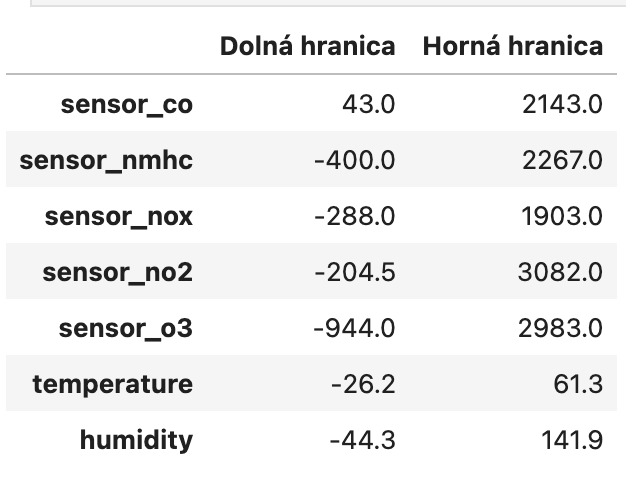
\includegraphics[width=\linewidth,keepaspectratio]{data_hranice_odlahlych_hodnot_tabulka.png}
\end{minipage}\hfill%
\begin{minipage}[c]{0.46\linewidth}
\raggedright
% main.ipynb: bunka 33
Na trénovacích dátach toto pravidlo odstraňuje \textbf{23 riadkov}, model sa učí na \textbf{5852 meraniach}. Test zostáva so všetkými 1469 riadkami.

Hranice v tabuľke boli naučené na finálnej tréningovej množine. Vo vnútornej CV sa počítajú osobitne pre každý tréningový fold.
\end{minipage}
\end{center}

% main.ipynb: bunka 34
\section{Trénovanie ML modelov}

% main.ipynb: bunka 34
Reziduál definujem ako skutočná mínus predpovedaná. Kladný reziduál znamená podhodnotenie, záporný nadhodnotenie.

% main.ipynb: bunka 34
Model vyberiem podľa najnižšej priemernej \textbf{CV MSE}. CV smerodajná odchýlka je variabilita medzi foldmi, nie interval spoľahlivosti.

% main.ipynb: bunka 34
Pri strome ladím hĺbku a minimálny počet vzoriek v liste. Random Forest priemeruje bootstrapové stromy, ExtraTrees (Extremely Randomized Trees) navyše náhodne volí prahy. XGBoost a histogramový boosting pridávajú stromy postupne na opravu predchádzajúcich chýb. Pri SVR volím regresnú verziu SVM s RBF jadrom, penalizáciou C, šírkou jadra gamma a toleranciou epsilon.

% main.ipynb: bunka 35
Pri 3-fold CV sa každá konfigurácia trénuje trikrát na dvoch foldoch a hodnotí na zostávajúcom.

\begin{center}
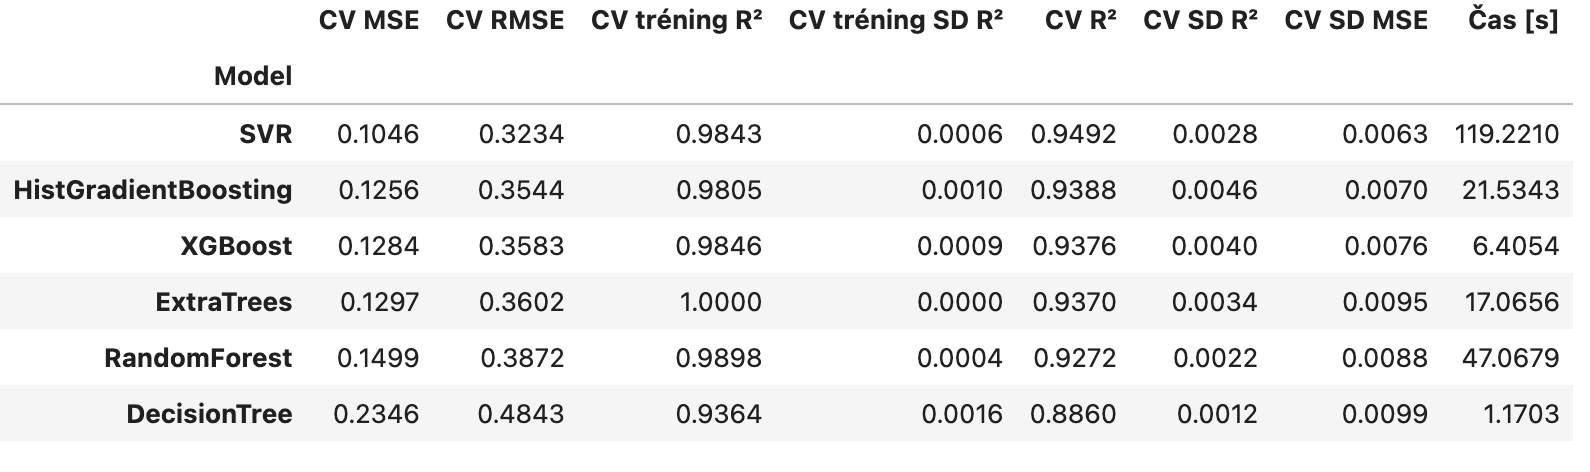
\includegraphics[width=\linewidth,keepaspectratio]{modely_porovnanie_cv_tabulka.png}
\end{center}

% main.ipynb: bunka 40
DecisionTree, RandomForest, ExtraTrees a XGBoost používajú natívnu dôležitosť kódovaných vstupov. HistGradientBoosting a SVR používajú permutáciu pôvodných stĺpcov.

\subsection{DecisionTree}

% main.ipynb: bunka 110
Najlepší strom podľa CV má hĺbku \textbf{8} a aspoň \textbf{8} vzoriek v liste.

\begin{center}
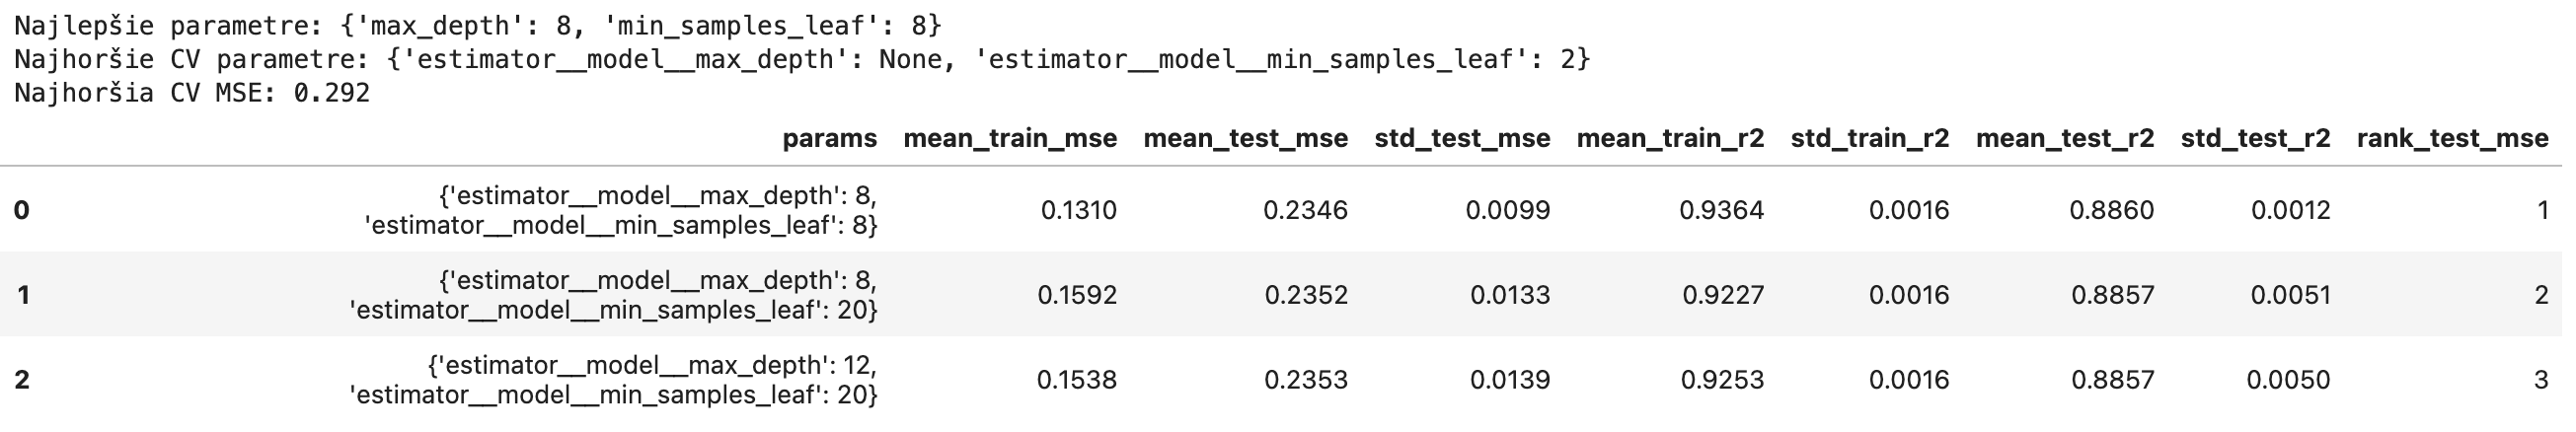
\includegraphics[width=\linewidth,keepaspectratio]{decision_tree_ladenie_tabulka.png}
\end{center}

\begin{center}
\noindent
\begin{minipage}[c]{0.44\linewidth}
\centering
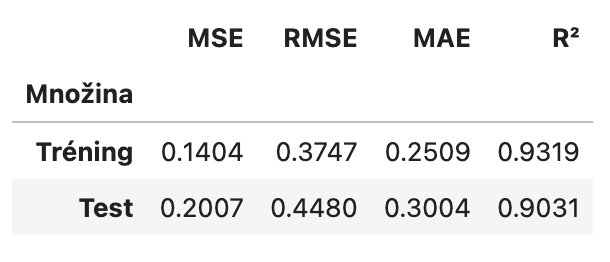
\includegraphics[width=0.7\linewidth,keepaspectratio]{decision_tree_metriky_tabulka.png}
\medskip
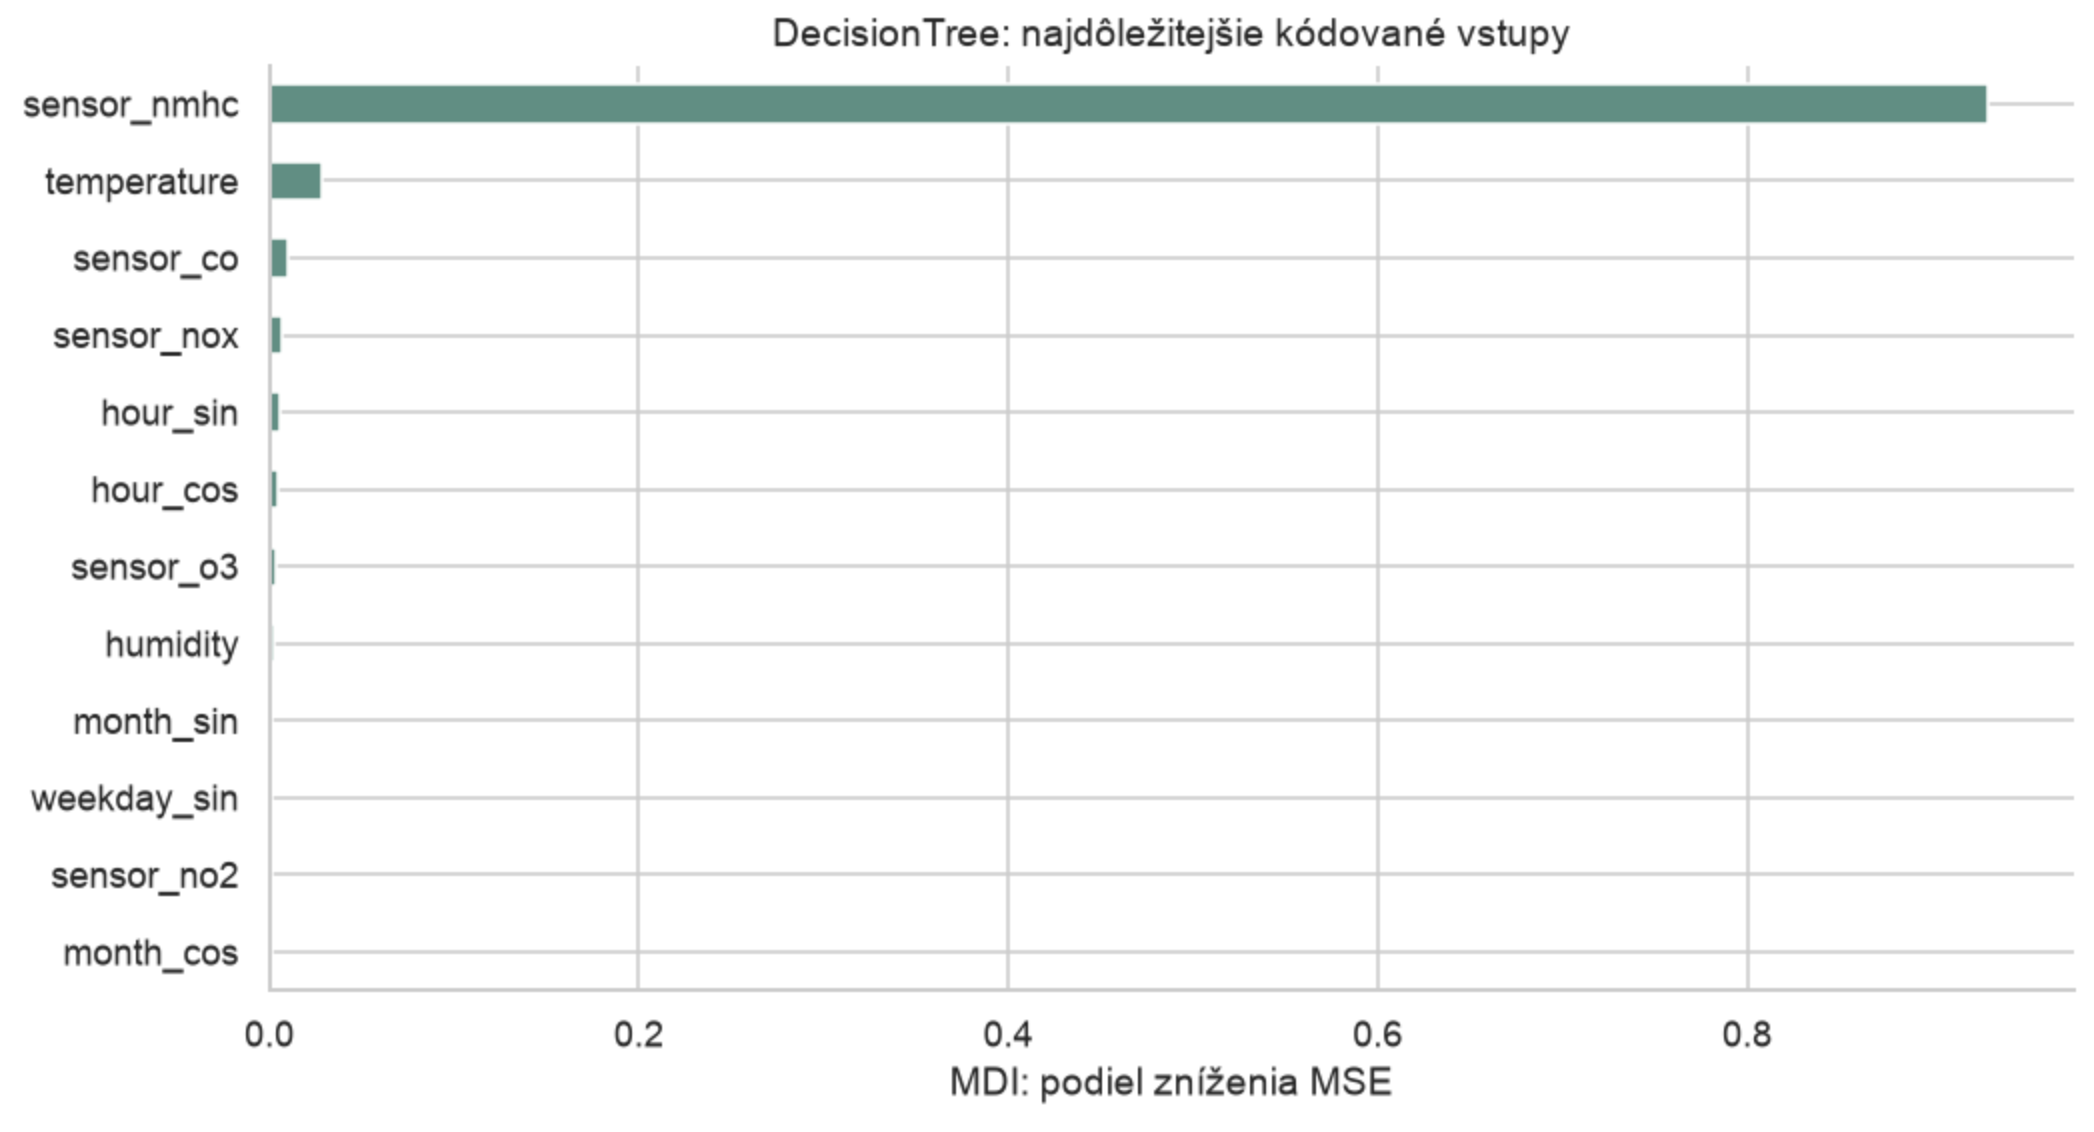
\includegraphics[width=\linewidth,keepaspectratio]{decision_tree_dolezitost_priznakov_graf.png}
\end{minipage}\hfill%
\begin{minipage}[c]{0.53\linewidth}
\centering
\small\textbf{Dôležitosť príznakov}\par\smallskip
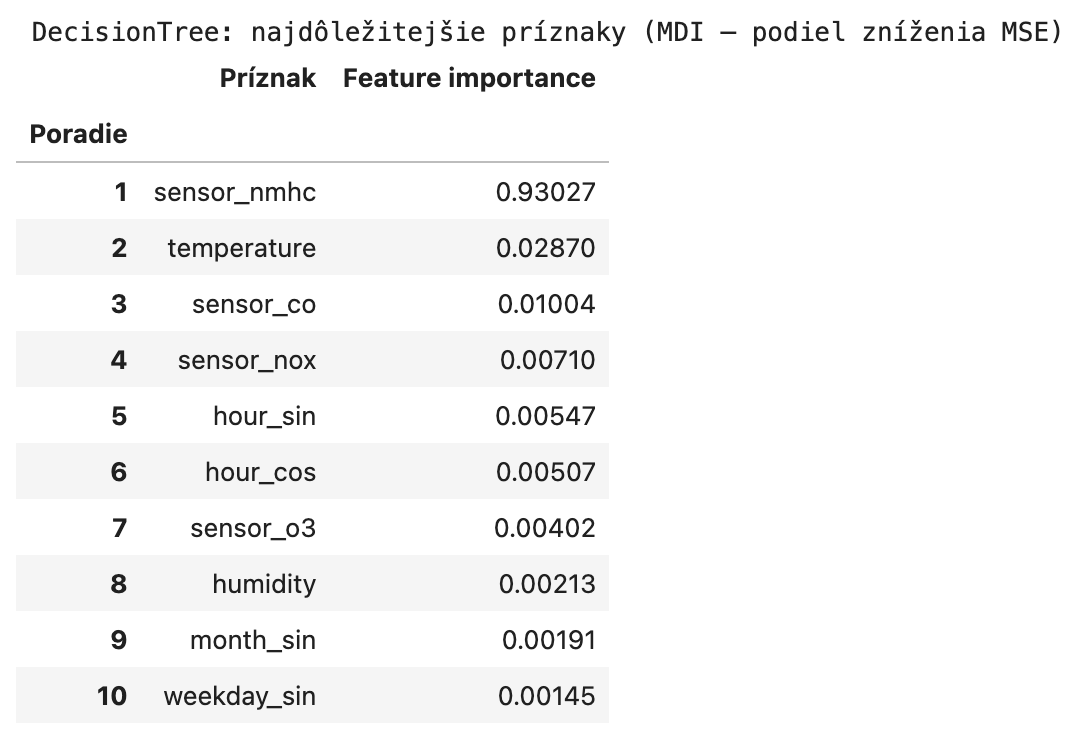
\includegraphics[width=0.6\linewidth,keepaspectratio,trim=5.5bp 7bp 238bp 30.5bp,clip]{decision_tree_dolezitost_priznakov_tabulka.png}
\end{minipage}
\end{center}

% main.ipynb: bunka 43
\textbf{DecisionTree} má tréningové \(R^2\) \textbf{0.9319} a testovacie \(R^2\) \textbf{0.9031}. Testovacia RMSE je \textbf{0.4480 \(\mathrm{mg}/\mathrm{m}^3\)}, MAE 0.3004 \(\mathrm{mg}/\mathrm{m}^3\). Rozdiel tréningového a testovacieho \(R^2\) je 0.0288. Rozdiel je menší než pri výrazne preučených ensemble modeloch.

% main.ipynb: bunka 47
Najvyššiu natívnu dôležitosť modelu \textbf{DecisionTree} má \textbf{sensor\_nmhc}, MDI \textbf{0.93027}. Prvé tri vstupy spolu získali \textbf{96.90\%} relatívnej dôležitosti.

% main.ipynb: bunka 50
\subsubsection{Vizualizácia malého rozhodovacieho stromu}

% main.ipynb: bunka 50
Pre čitateľnosť natrénujem samostatný ilustračný strom s hĺbkou 3 a minimálne 30 meraniami v liste. Použijem sedem pôvodných spojitých vstupov bez škálovania, aby prahy mali zrozumiteľné jednotky. Jeho parametre a výsledok sú odlíšené od ladeného stromu. V liste \texttt{value} znamená priemerné CO a \texttt{squared\_\allowbreak{}error} priemernú štvorcovú odchýlku cieľa v danom uzle.

\begin{center}
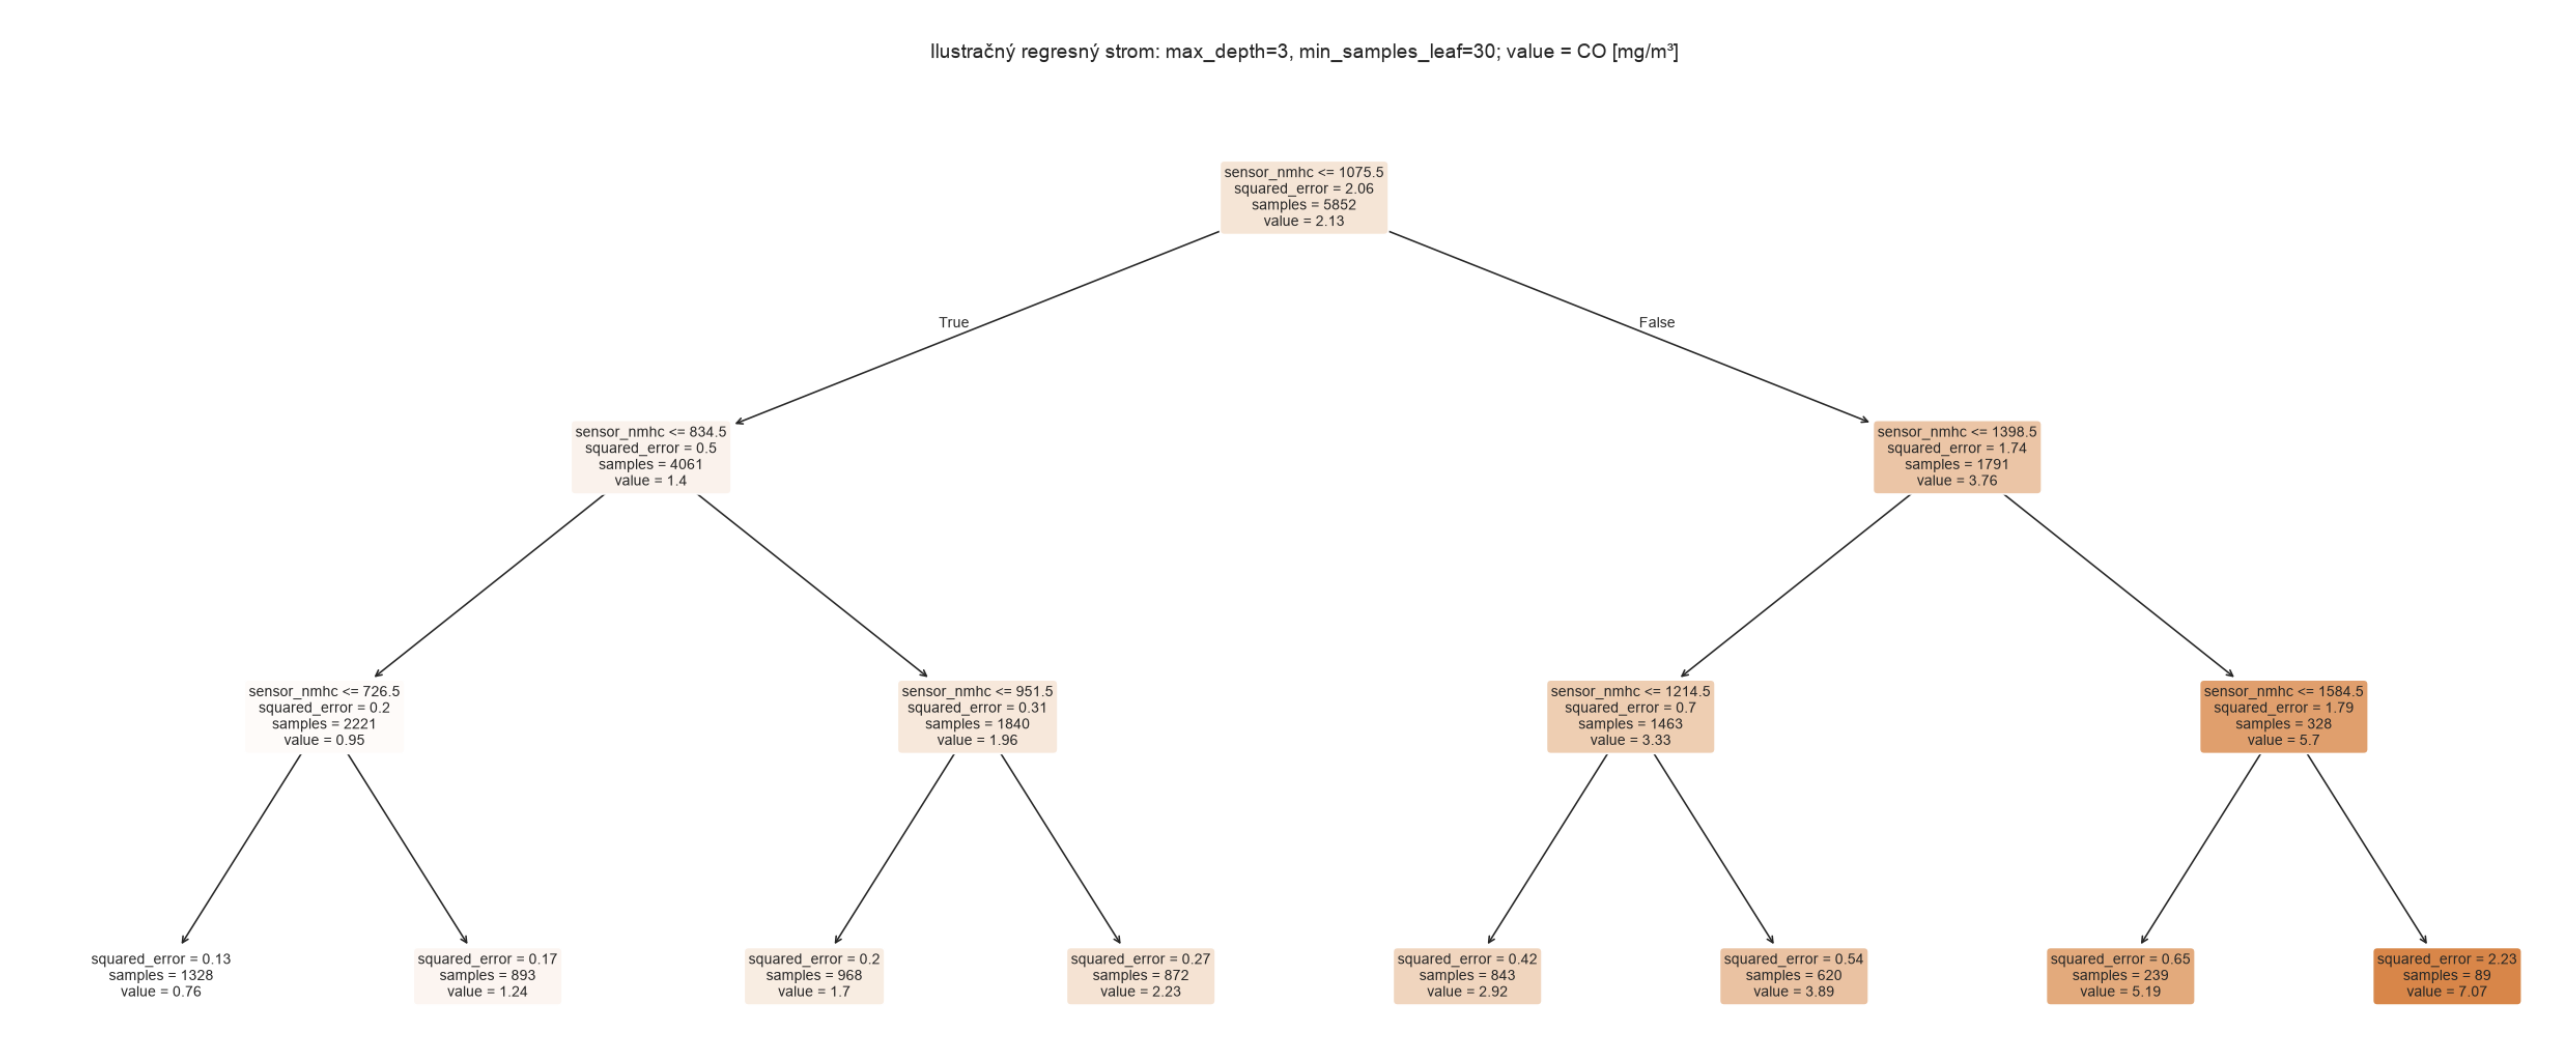
\includegraphics[width=\linewidth,keepaspectratio]{decision_tree_ilustracny_strom_graf.png}
\end{center}

% main.ipynb: bunka 52
Koreň delí podľa \textbf{\(\mathrm{sensor\_nmhc} \le 1075.50\)}. Ľavá vetva zodpovedá splneniu podmienky, pravá jej nesplneniu. Ilustračný strom dosahuje testovacie \(R^2\) \textbf{0.8394} a RMSE 0.5769 \(\mathrm{mg}/\mathrm{m}^3\). Je plytký, preto ukazuje hlavné pravidlá, ale nezachytáva všetky jemné interakcie.

% main.ipynb: bunka 53
Tabuľka pri výsledkoch ladeného \textbf{DecisionTree} opisuje ladený model. Malý ilustračný strom používa pôvodné spojité vstupy. Má inú hĺbku aj výsledky než ladený model, preto ich interpretáciu rozlišujem.

\subsection{Ensemble}

% main.ipynb: bunka 54
Súborové modely kombinujú viac stromov. Random Forest a ExtraTrees ich predikcie priemerujú. XGBoost a HistGradientBoosting vytvárajú postupnosť korekcií.

\subsubsection{RandomForest}

\begin{center}
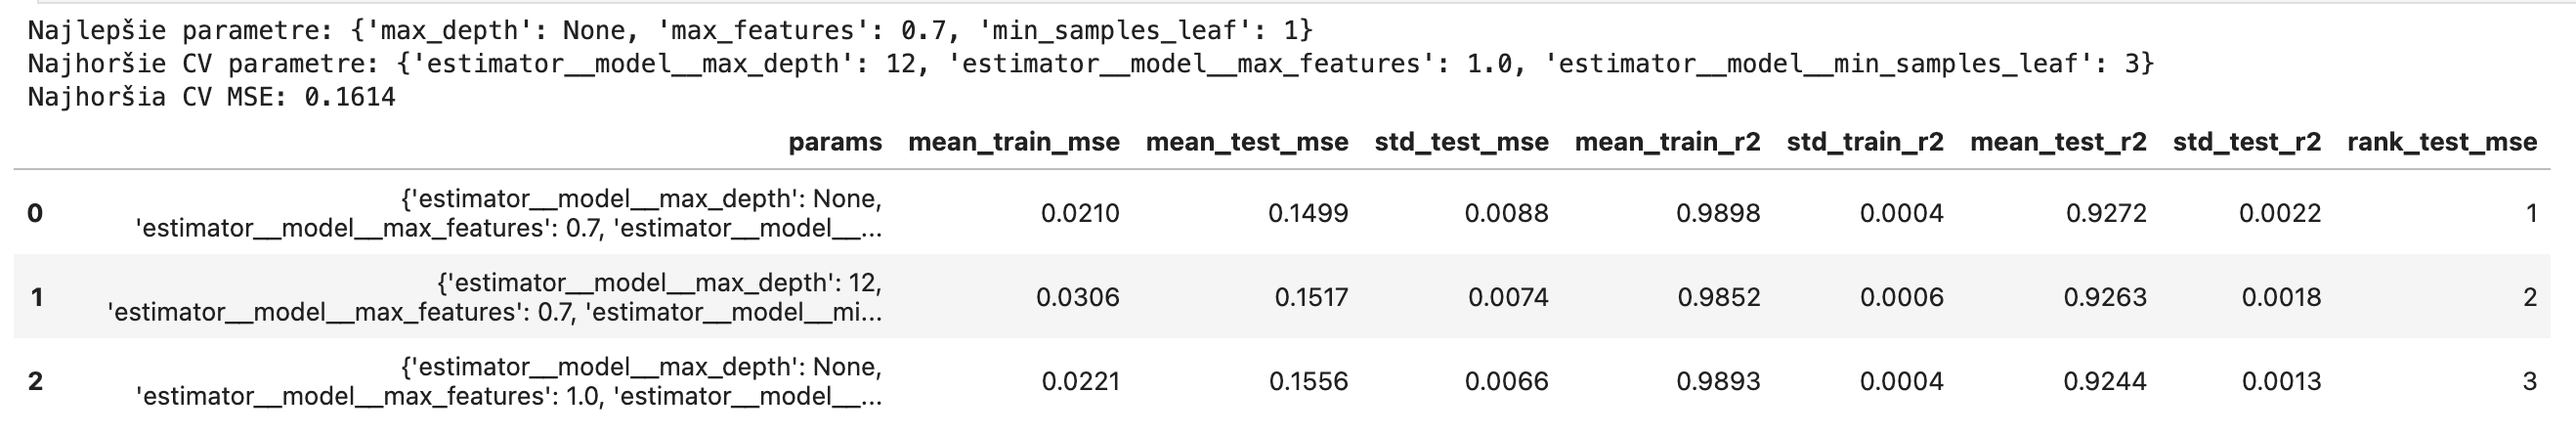
\includegraphics[width=\linewidth,keepaspectratio]{random_forest_ladenie_tabulka.png}
\end{center}

\begin{center}
\noindent
\begin{minipage}[c]{0.44\linewidth}
\centering
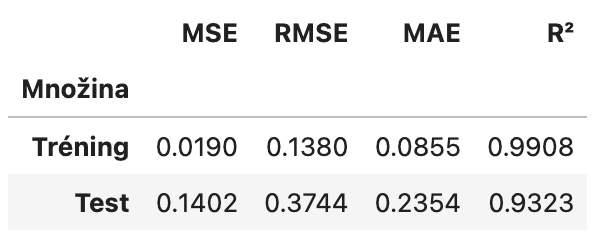
\includegraphics[width=0.7\linewidth,keepaspectratio]{random_forest_metriky_tabulka.png}
\medskip
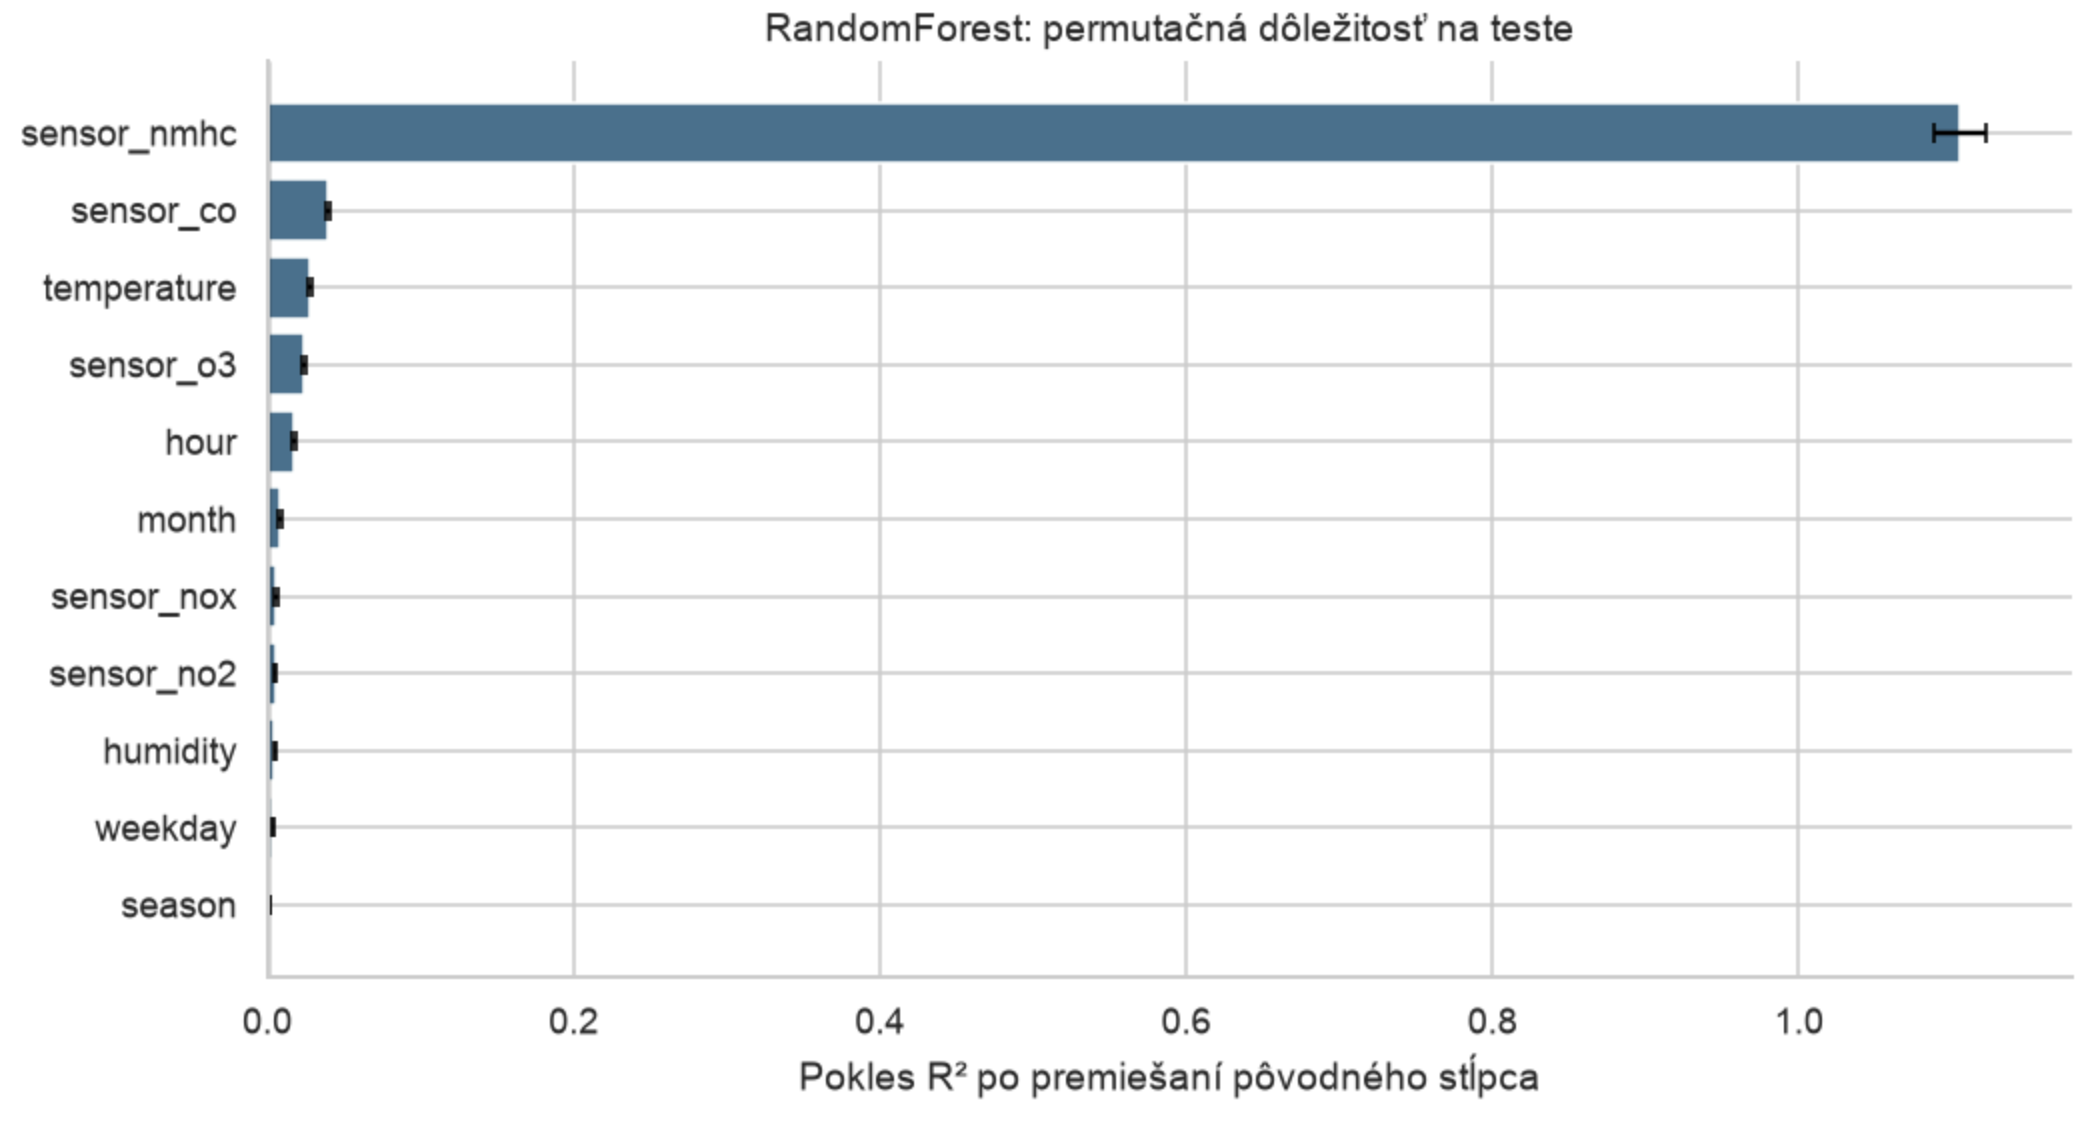
\includegraphics[width=\linewidth,keepaspectratio]{random_forest_permutacna_dolezitost_graf.png}
\end{minipage}\hfill%
\begin{minipage}[c]{0.53\linewidth}
\centering
\small\textbf{Dôležitosť príznakov}\par\smallskip
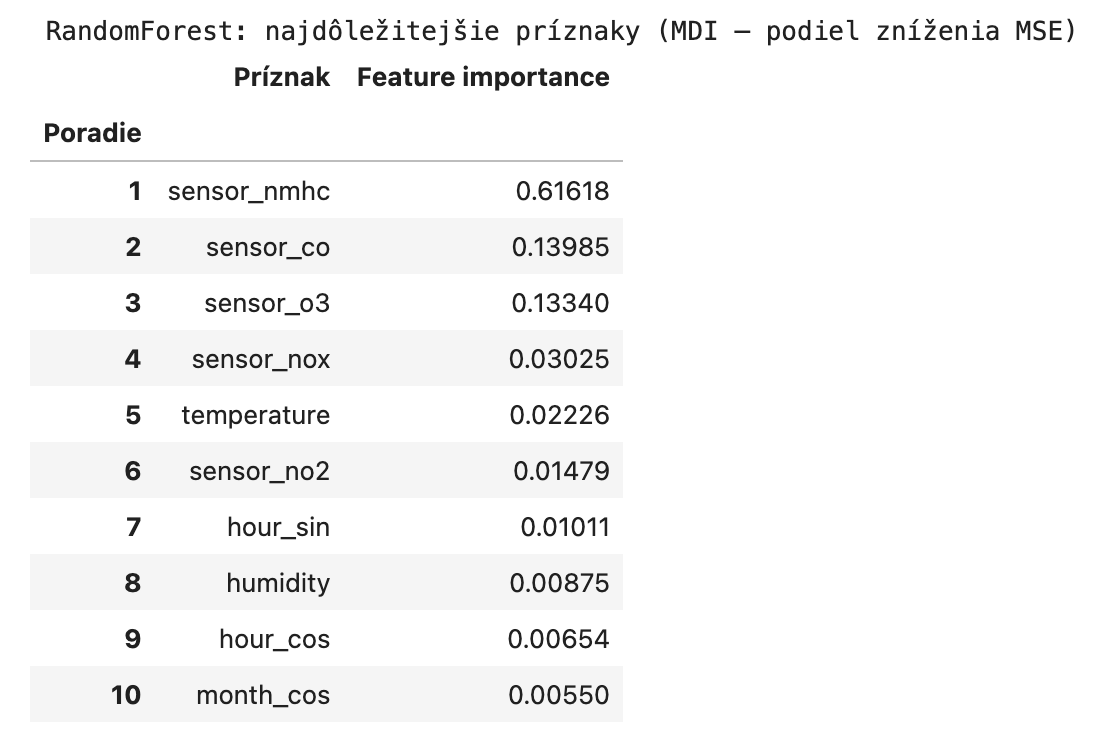
\includegraphics[width=0.5\linewidth,keepaspectratio,trim=12.5bp 8.5bp 233bp 30bp,clip]{random_forest_dolezitost_priznakov_tabulka.png}
\end{minipage}
\end{center}

% main.ipynb: bunka 57
\textbf{RandomForest} má tréningové \(R^2\) \textbf{0.9908} a testovacie \(R^2\) \textbf{0.9323}. Testovacia RMSE je \textbf{0.3744 \(\mathrm{mg}/\mathrm{m}^3\)}, MAE 0.2354 \(\mathrm{mg}/\mathrm{m}^3\). Rozdiel tréningového a testovacieho \(R^2\) je 0.0584. Rozdiel upozorňuje na preučenie oproti prispôsobeniu tréningu.

% main.ipynb: bunka 64
Les obsahuje \textbf{200 stromov}.

\subsubsection{Viacero stromov z ladeného Random Forestu}

% main.ipynb: bunka 62
Zobrazím tri skutočné stromy lesa. Každý obrázok ukazuje výrez do hĺbky 3, \texttt{(...)} označuje pokračovanie. Prahy sú v štandardizovaných jednotkách z. Číslo stromu je jeho poradie v lese. Predikcia lesa je priemer predikcií všetkých 200 stromov.

\begin{center}
\noindent
\begin{minipage}[c]{0.62\linewidth}
\centering
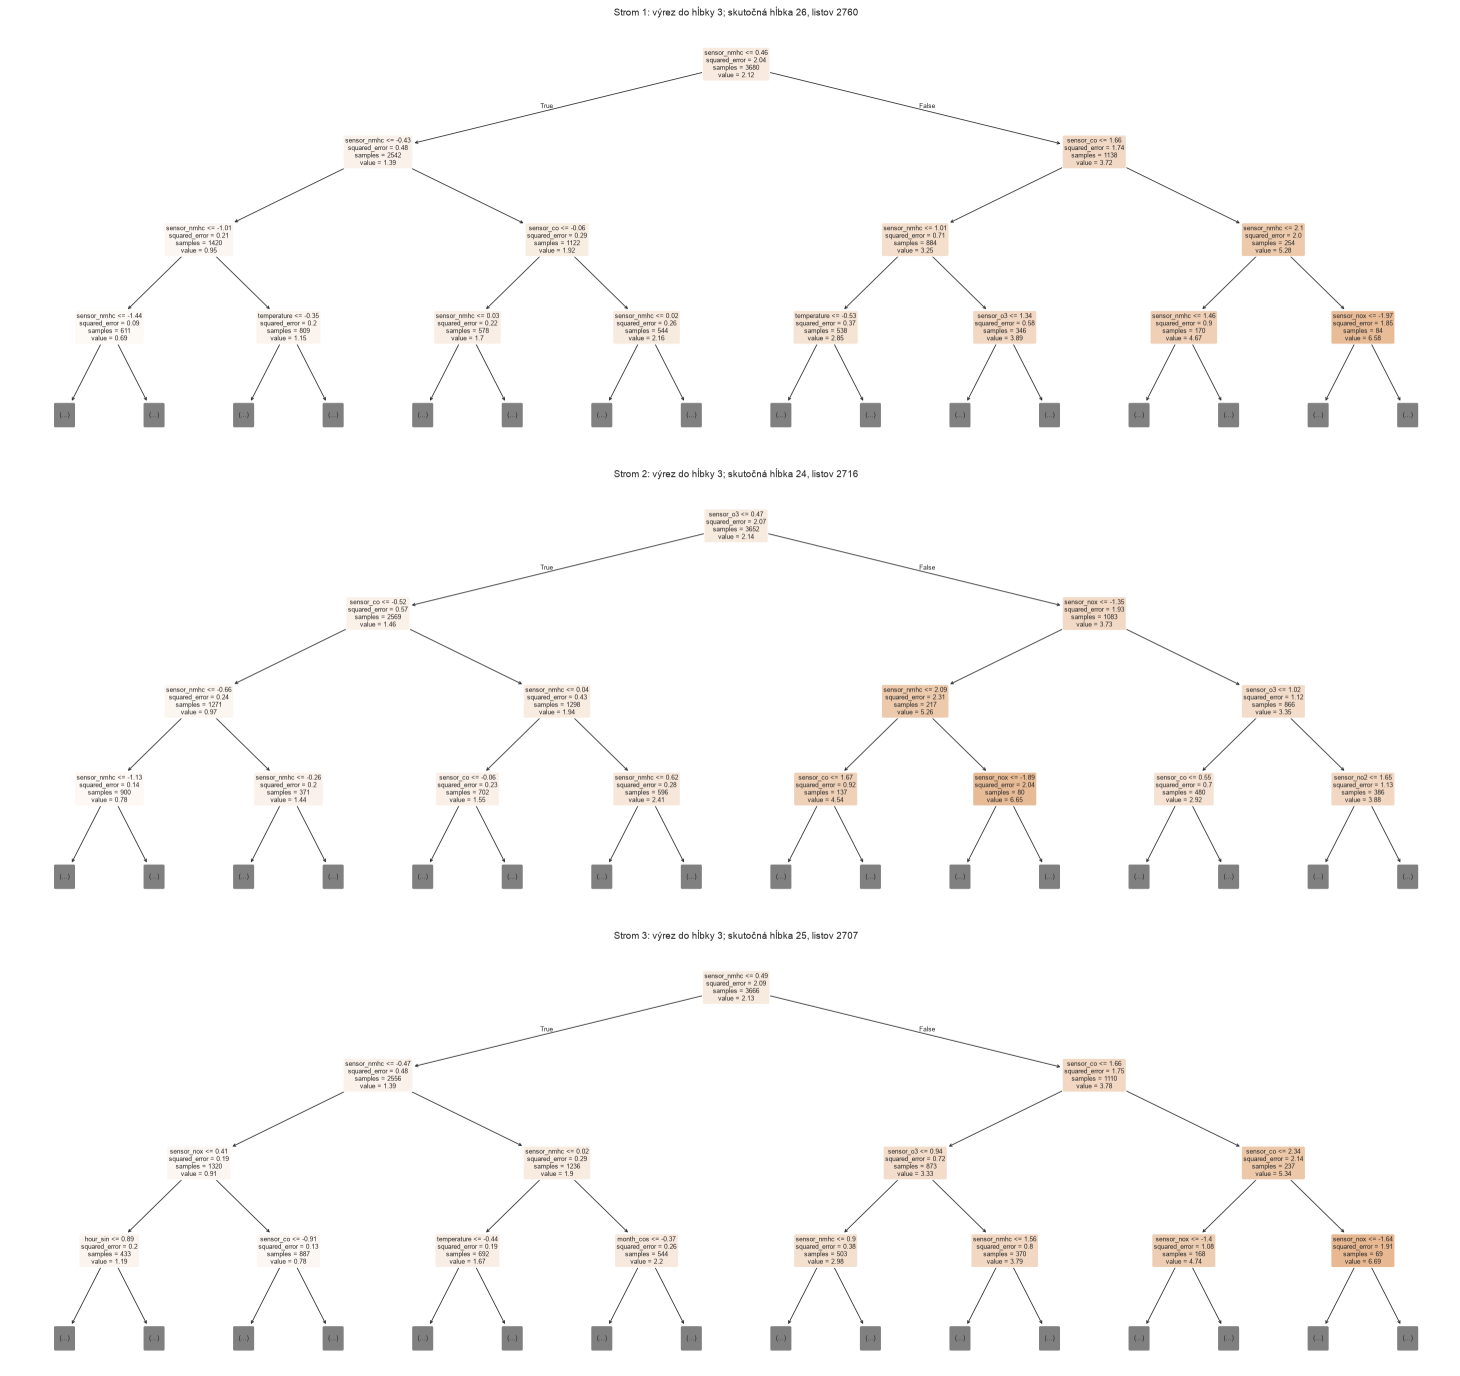
\includegraphics[width=\linewidth,keepaspectratio]{random_forest_vybrane_stromy_graf.png}
\end{minipage}\hfill%
\begin{minipage}[c]{0.35\linewidth}
\centering
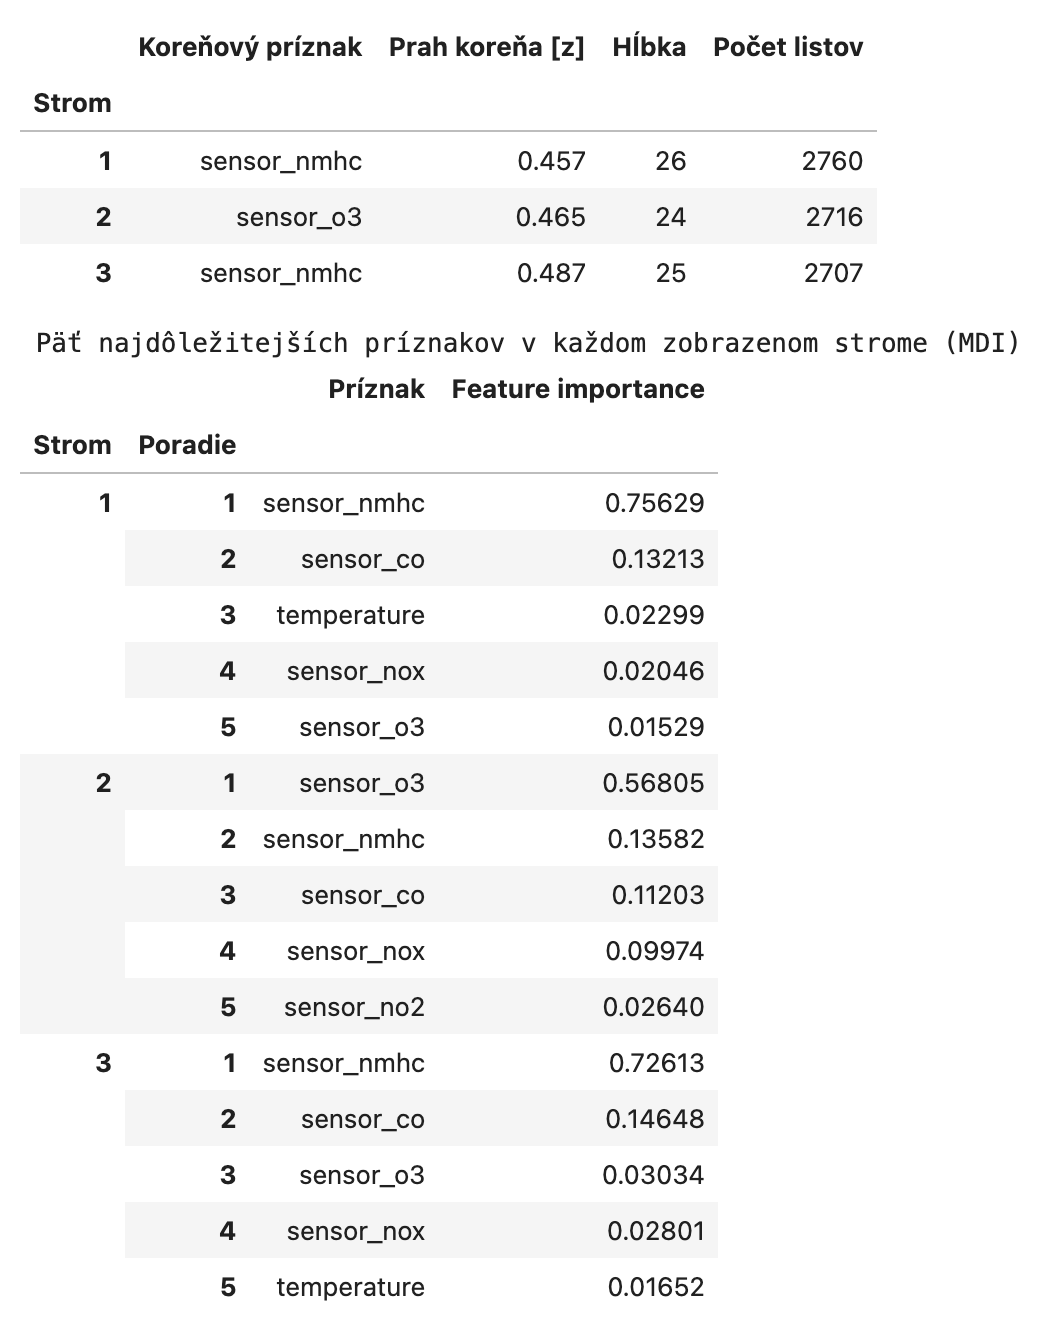
\includegraphics[width=\linewidth,keepaspectratio]{random_forest_vybrane_stromy_tabulka.png}
\end{minipage}
\end{center}


% main.ipynb: bunka 64
Les obsahuje \textbf{200 stromov}. Zobrazené stromy majú hĺbky \textbf{26, 24, 25} a korene podľa \textbf{sensor\_nmhc, sensor\_o3, sensor\_nmhc}. Tabuľka porovnáva aj prahy a počty listov. Rozdiely vznikajú bootstrapovými vzorkami a náhodným výberom príznakov. Obrázky ukazujú iba začiatky stromov. Výslednú predikciu tvorí priemer celého lesa.

\subsubsection{ExtraTrees}

\begin{center}
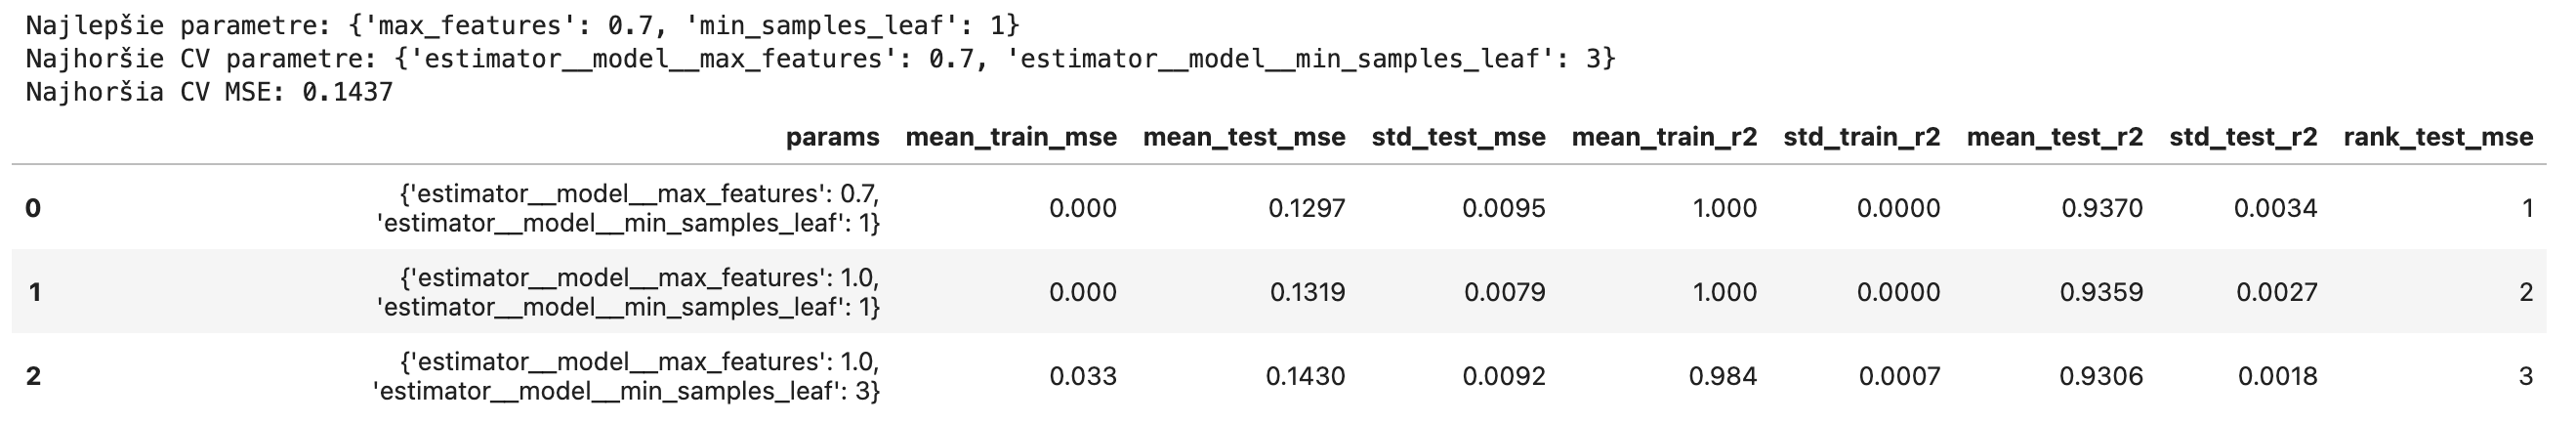
\includegraphics[width=\linewidth,keepaspectratio]{extra_trees_ladenie_tabulka.png}
\end{center}

\begin{center}
\noindent
\begin{minipage}[c]{0.44\linewidth}
\centering
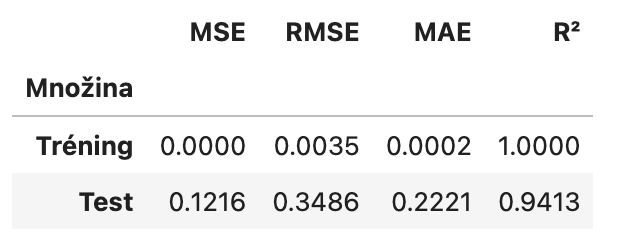
\includegraphics[width=\linewidth,keepaspectratio]{extra_trees_metriky_tabulka.png}
\end{minipage}\hfill%
\begin{minipage}[c]{0.53\linewidth}
\centering
\small\textbf{Dôležitosť príznakov}\par\smallskip
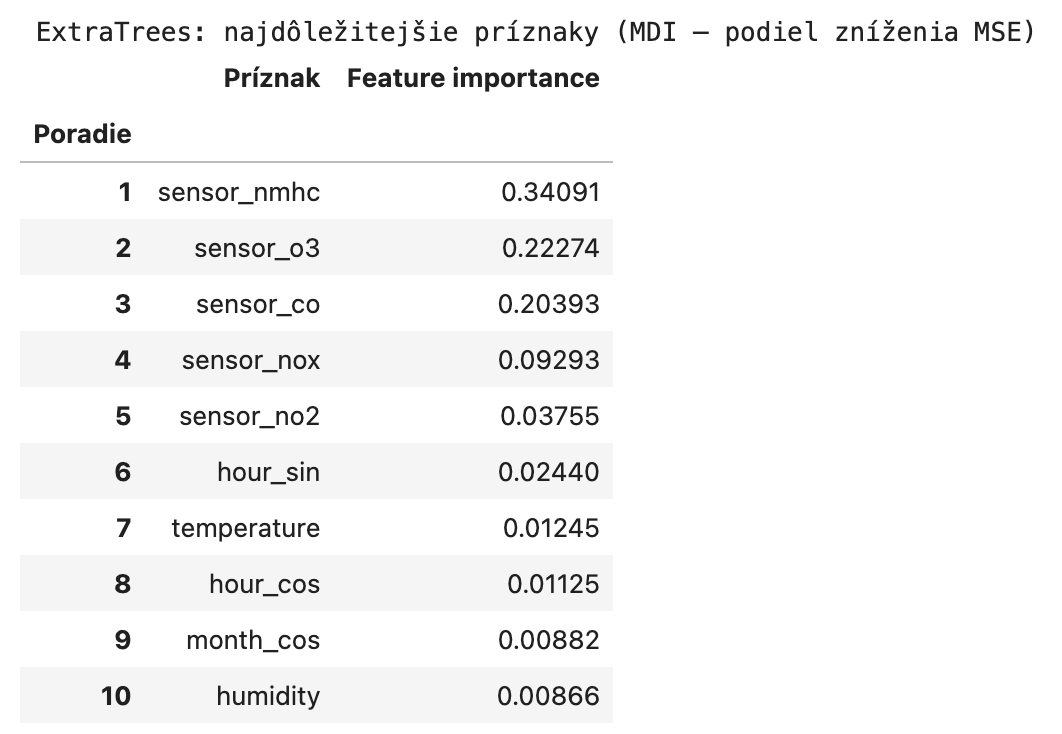
\includegraphics[width=0.5\linewidth,keepaspectratio,trim=7.5bp 3bp 222bp 30.5bp,clip]{extra_trees_dolezitost_priznakov_tabulka.png}
\end{minipage}
\end{center}

% main.ipynb: bunka 73
\textbf{ExtraTrees} má tréningové \(R^2\) \textbf{1.0000} a testovacie \(R^2\) \textbf{0.9413}. Testovacia RMSE je \textbf{0.3486 \(\mathrm{mg}/\mathrm{m}^3\)}, MAE 0.2221 \(\mathrm{mg}/\mathrm{m}^3\). Rozdiel tréningového a testovacieho \(R^2\) je 0.0587. Takmer nulová tréningová chyba pri nenulovej testovacej ukazuje silné zapamätanie tréningových meraní.

% main.ipynb: bunka 77
Najvyššiu natívnu dôležitosť modelu \textbf{ExtraTrees} má \textbf{sensor\_nmhc}, MDI \textbf{0.34091}. Prvé tri vstupy spolu získali \textbf{76.76\%} relatívnej dôležitosti.

\subsubsection{XGBoost}

\begin{center}
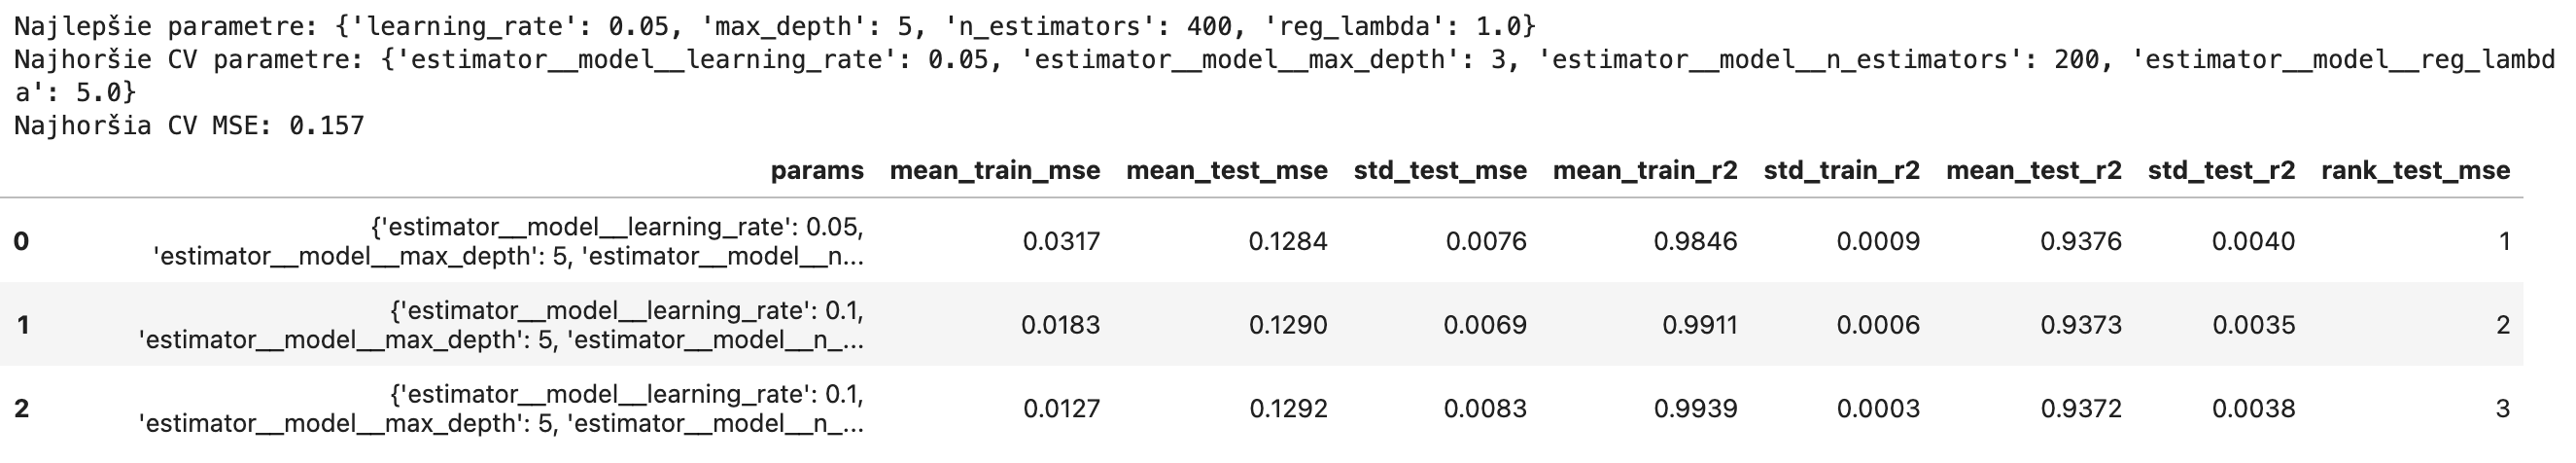
\includegraphics[width=\linewidth,keepaspectratio]{xgboost_ladenie_tabulka.png}
\end{center}

\begin{center}
\noindent
\begin{minipage}[c]{0.44\linewidth}
\centering
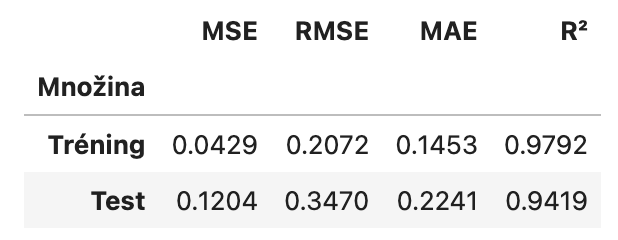
\includegraphics[width=\linewidth,keepaspectratio]{xgboost_metriky_tabulka.png}
\end{minipage}\hfill%
\begin{minipage}[c]{0.53\linewidth}
\centering
\small\textbf{Dôležitosť príznakov}\par\smallskip
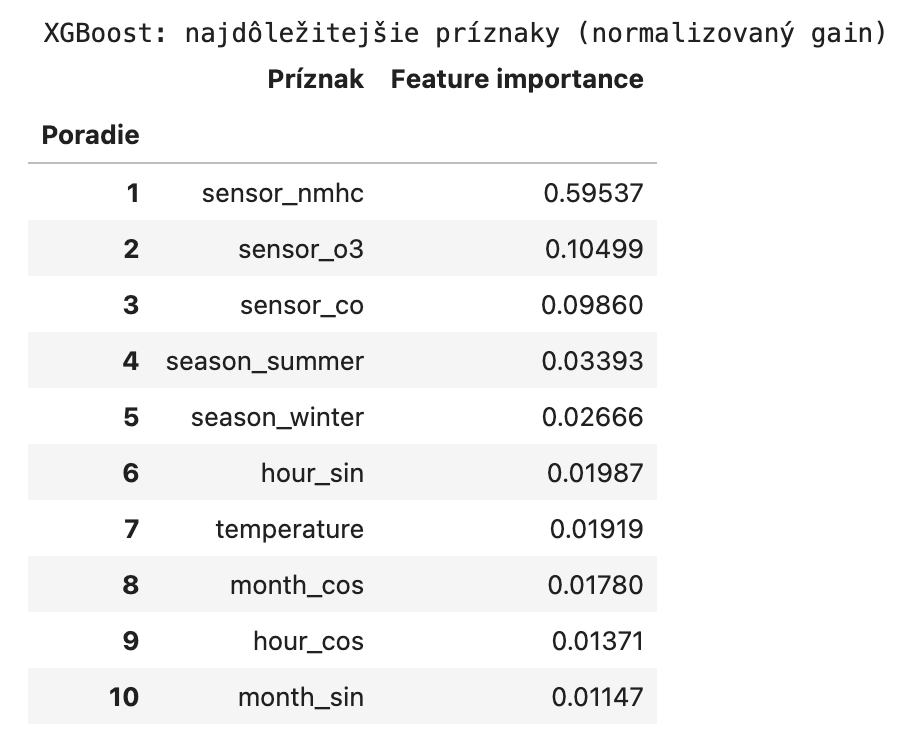
\includegraphics[width=0.5\linewidth,keepaspectratio,trim=11.5bp 0.5bp 118bp 31bp,clip]{xgboost_dolezitost_priznakov_tabulka.png}
\end{minipage}
\end{center}

% main.ipynb: bunka 82
\textbf{XGBoost} má tréningové \(R^2\) \textbf{0.9792} a testovacie \(R^2\) \textbf{0.9419}. Testovacia RMSE je \textbf{0.3470 \(\mathrm{mg}/\mathrm{m}^3\)}, MAE 0.2241 \(\mathrm{mg}/\mathrm{m}^3\). Rozdiel tréningového a testovacieho \(R^2\) je 0.0373. Rozdiel je menší než pri výrazne preučených súborových modeloch.

% main.ipynb: bunka 86
Najvyššiu natívnu dôležitosť modelu \textbf{XGBoost} má \textbf{sensor\_nmhc}, normalizovaný gain \textbf{0.59537}. Prvé tri vstupy spolu získali \textbf{79.90\%} relatívnej dôležitosti.

\subsubsection{HistGradientBoosting}

\begin{center}
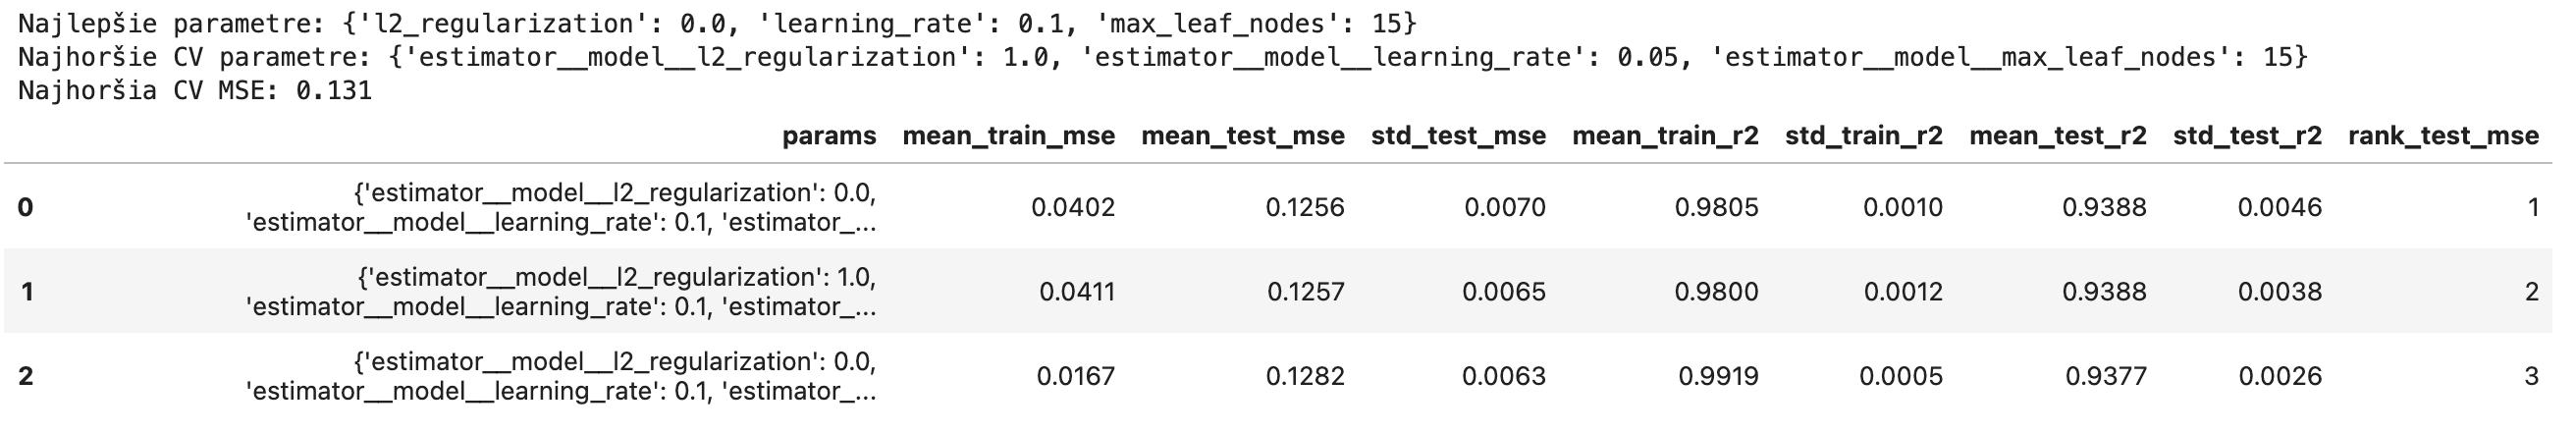
\includegraphics[width=\linewidth,keepaspectratio]{hist_gradient_boosting_ladenie_tabulka.png}
\end{center}

\begin{center}
\noindent
\begin{minipage}[c]{0.44\linewidth}
\centering
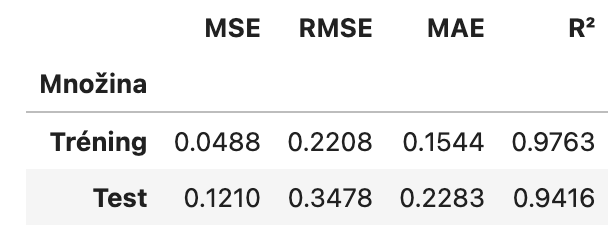
\includegraphics[width=\linewidth,keepaspectratio]{hist_gradient_boosting_metriky_tabulka.png}
\end{minipage}\hfill%
\begin{minipage}[c]{0.53\linewidth}
\centering
\small\textbf{Permutačná dôležitosť}\par\smallskip
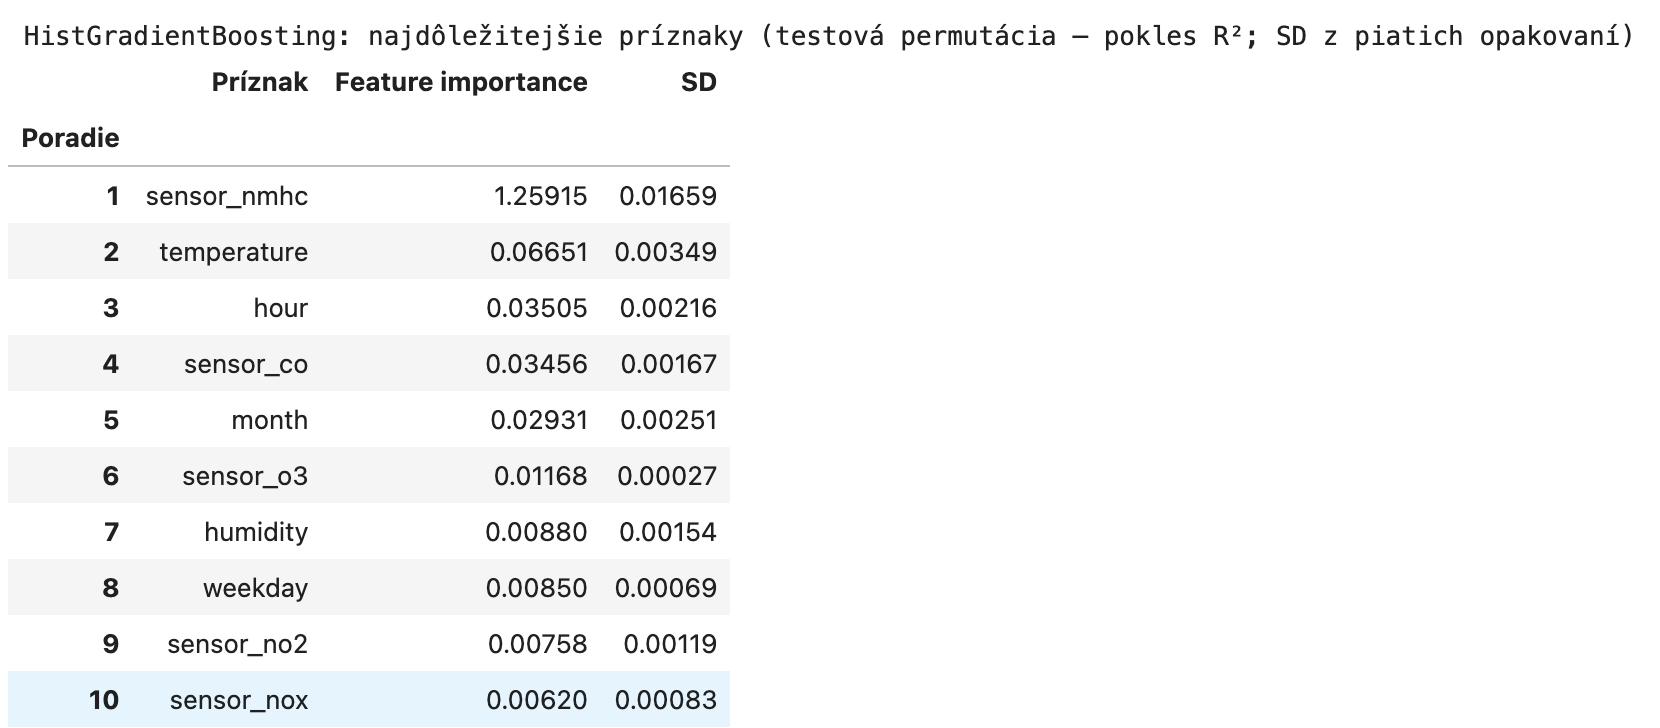
\includegraphics[width=0.5\linewidth,keepaspectratio,trim=1.5bp 0bp 462.5bp 32.5bp,clip]{hist_gradient_boosting_permutacna_dolezitost_tabulka.png}
\end{minipage}
\end{center}

% main.ipynb: bunka 91
\textbf{HistGradientBoosting} má tréningové \(R^2\) \textbf{0.9763} a testovacie \(R^2\) \textbf{0.9416}. Testovacia RMSE je \textbf{0.3478 \(\mathrm{mg}/\mathrm{m}^3\)}, MAE 0.2283 \(\mathrm{mg}/\mathrm{m}^3\). Rozdiel tréningového a testovacieho \(R^2\) je 0.0347. Rozdiel je menší než pri výrazne preučených súborových modeloch.

% main.ipynb: bunka 95
Po premiešaní \textbf{sensor\_nmhc} klesne testovacie R² modelu \textbf{HistGradientBoosting} v priemere o \textbf{1.2591 ± 0.0166}.


\subsection{SVR}

% main.ipynb: bunka 34
Pri SVR volím regresnú verziu SVM s RBF jadrom, penalizáciou C, šírkou jadra gamma a toleranciou epsilon.

% main.ipynb: bunka 110
SVR vybral \textbf{C=100.0}, \textbf{gamma=scale}, \textbf{epsilon=0.1}.

\begin{center}
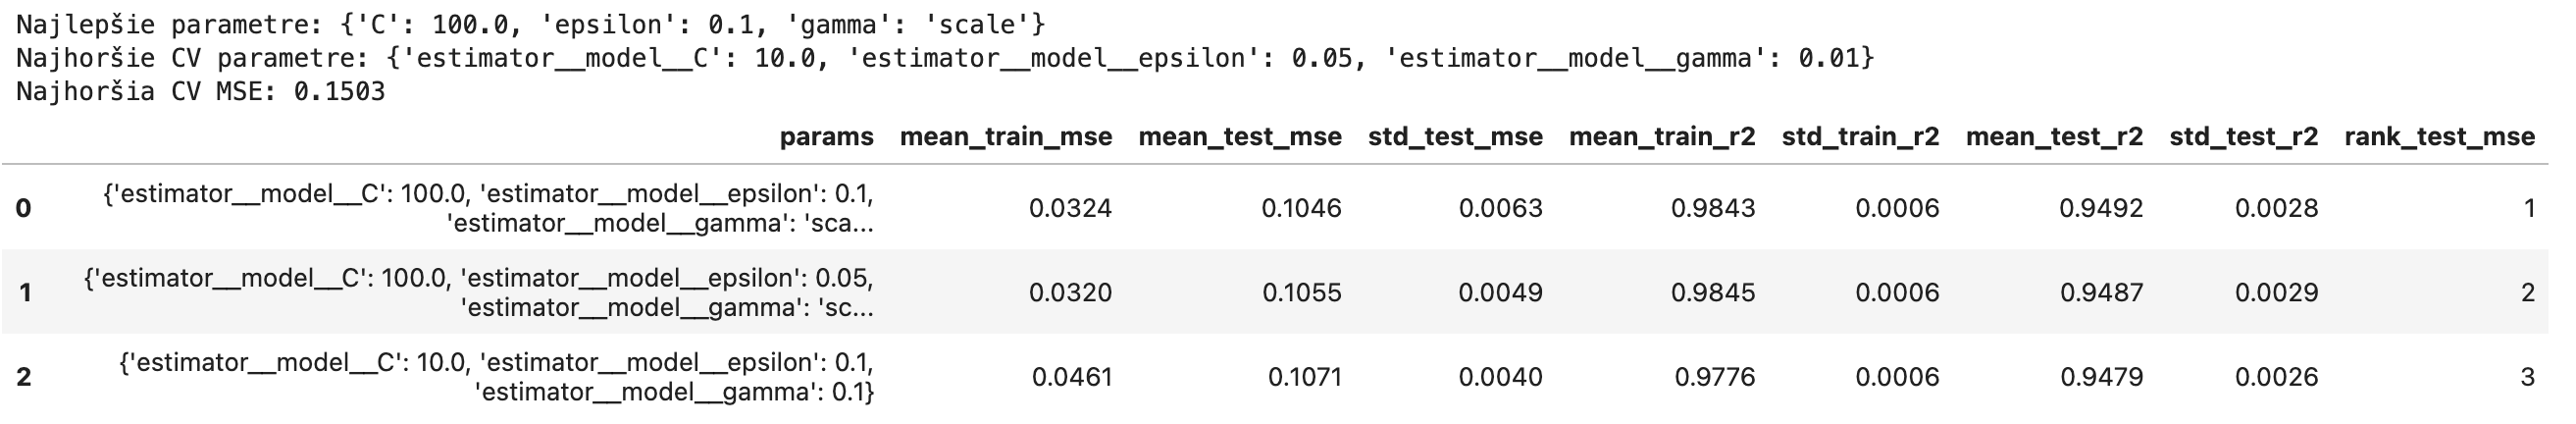
\includegraphics[width=\linewidth,keepaspectratio]{svr_ladenie_tabulka.png}
\end{center}

\begin{center}
\noindent
\begin{minipage}[c]{0.44\linewidth}
\centering
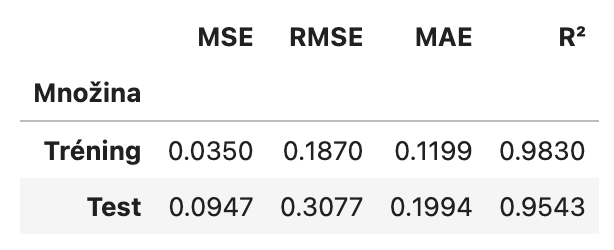
\includegraphics[width=\linewidth,keepaspectratio]{svr_metriky_tabulka.png}
\end{minipage}\hfill%
\begin{minipage}[c]{0.53\linewidth}
\centering
\small\textbf{Permutačná dôležitosť}\par\smallskip
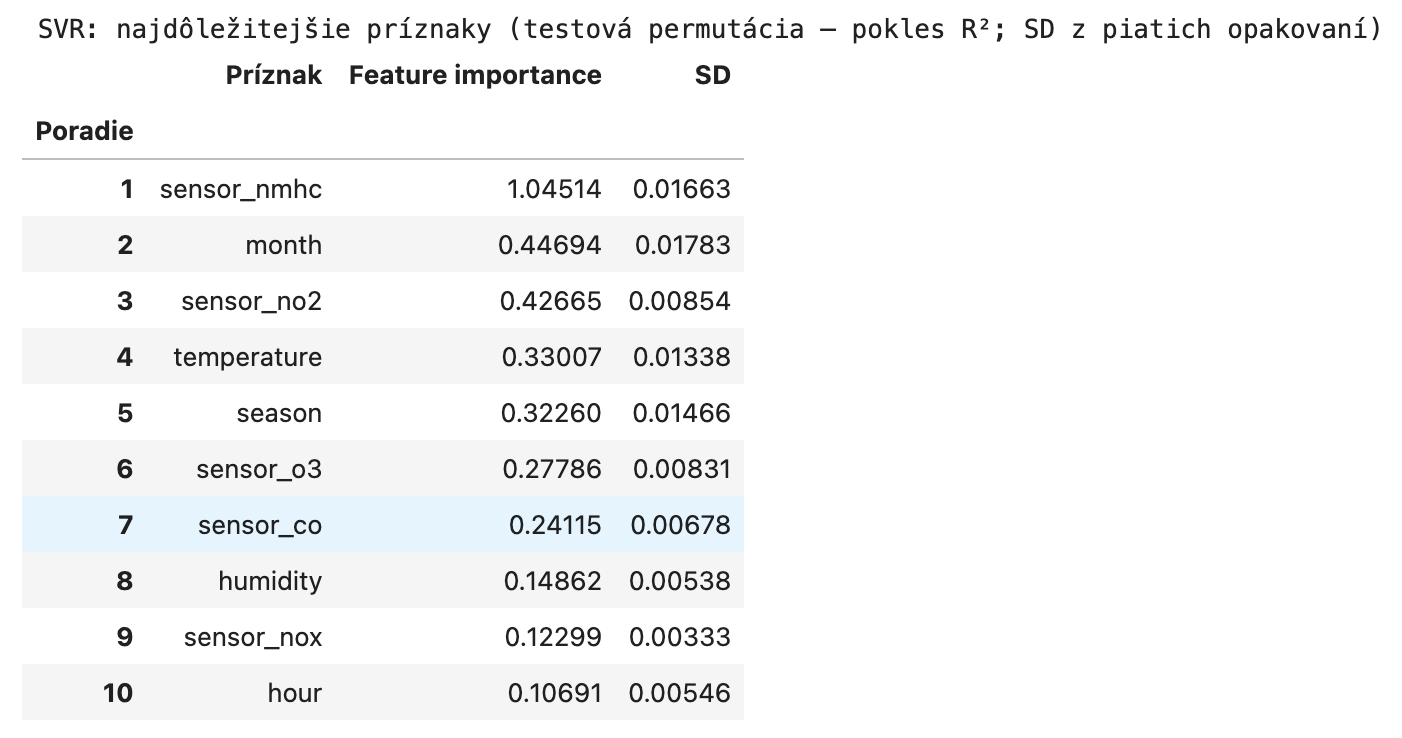
\includegraphics[width=0.5\linewidth,keepaspectratio,trim=8.5bp 6.5bp 326.5bp 29bp,clip]{svr_permutacna_dolezitost_tabulka.png}
\end{minipage}
\end{center}

% main.ipynb: bunka 98
\textbf{SVR} má tréningové \(R^2\) \textbf{0.9830} a testovacie \(R^2\) \textbf{0.9543}. Testovacia RMSE je \textbf{0.3077 \(\mathrm{mg}/\mathrm{m}^3\)}, MAE 0.1994 \(\mathrm{mg}/\mathrm{m}^3\). Rozdiel tréningového a testovacieho \(R^2\) je 0.0287. Rozdiel je menší než pri výrazne preučených súborových modeloch.

% main.ipynb: bunka 102
Po premiešaní \textbf{sensor\_nmhc} klesne testovacie R² modelu \textbf{SVR} v priemere o \textbf{1.0451 ± 0.0166}.

\subsection{Porovnanie reziduálov}

% main.ipynb: bunka 103
Všetky modely predikujú rovnakých 1 469 testovacích meraní.

\begin{center}
\noindent
\begin{minipage}[c]{0.49\linewidth}
\centering
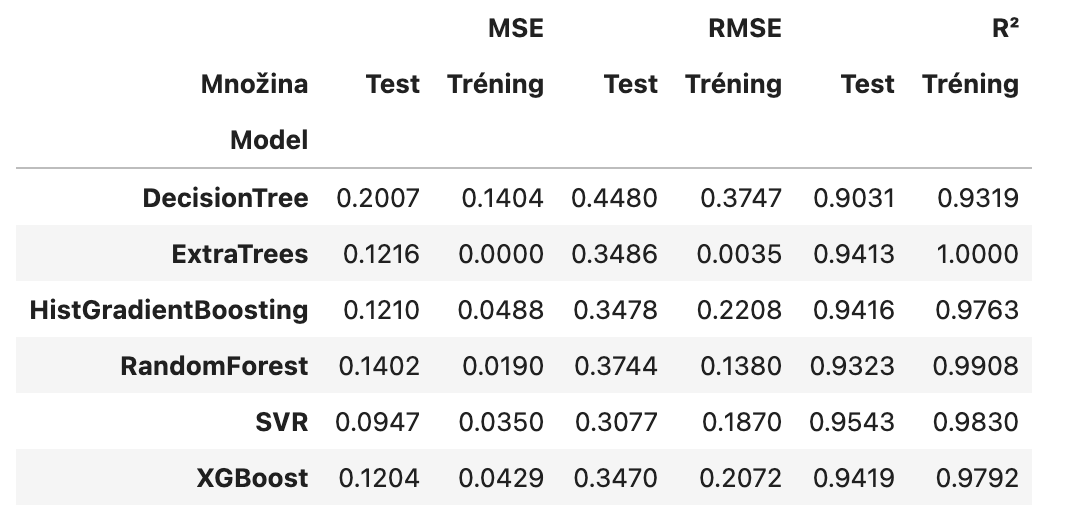
\includegraphics[width=\linewidth,keepaspectratio]{modely_porovnanie_metrik_tabulka.png}
\end{minipage}\hfill%
\begin{minipage}[c]{0.48\linewidth}
\centering
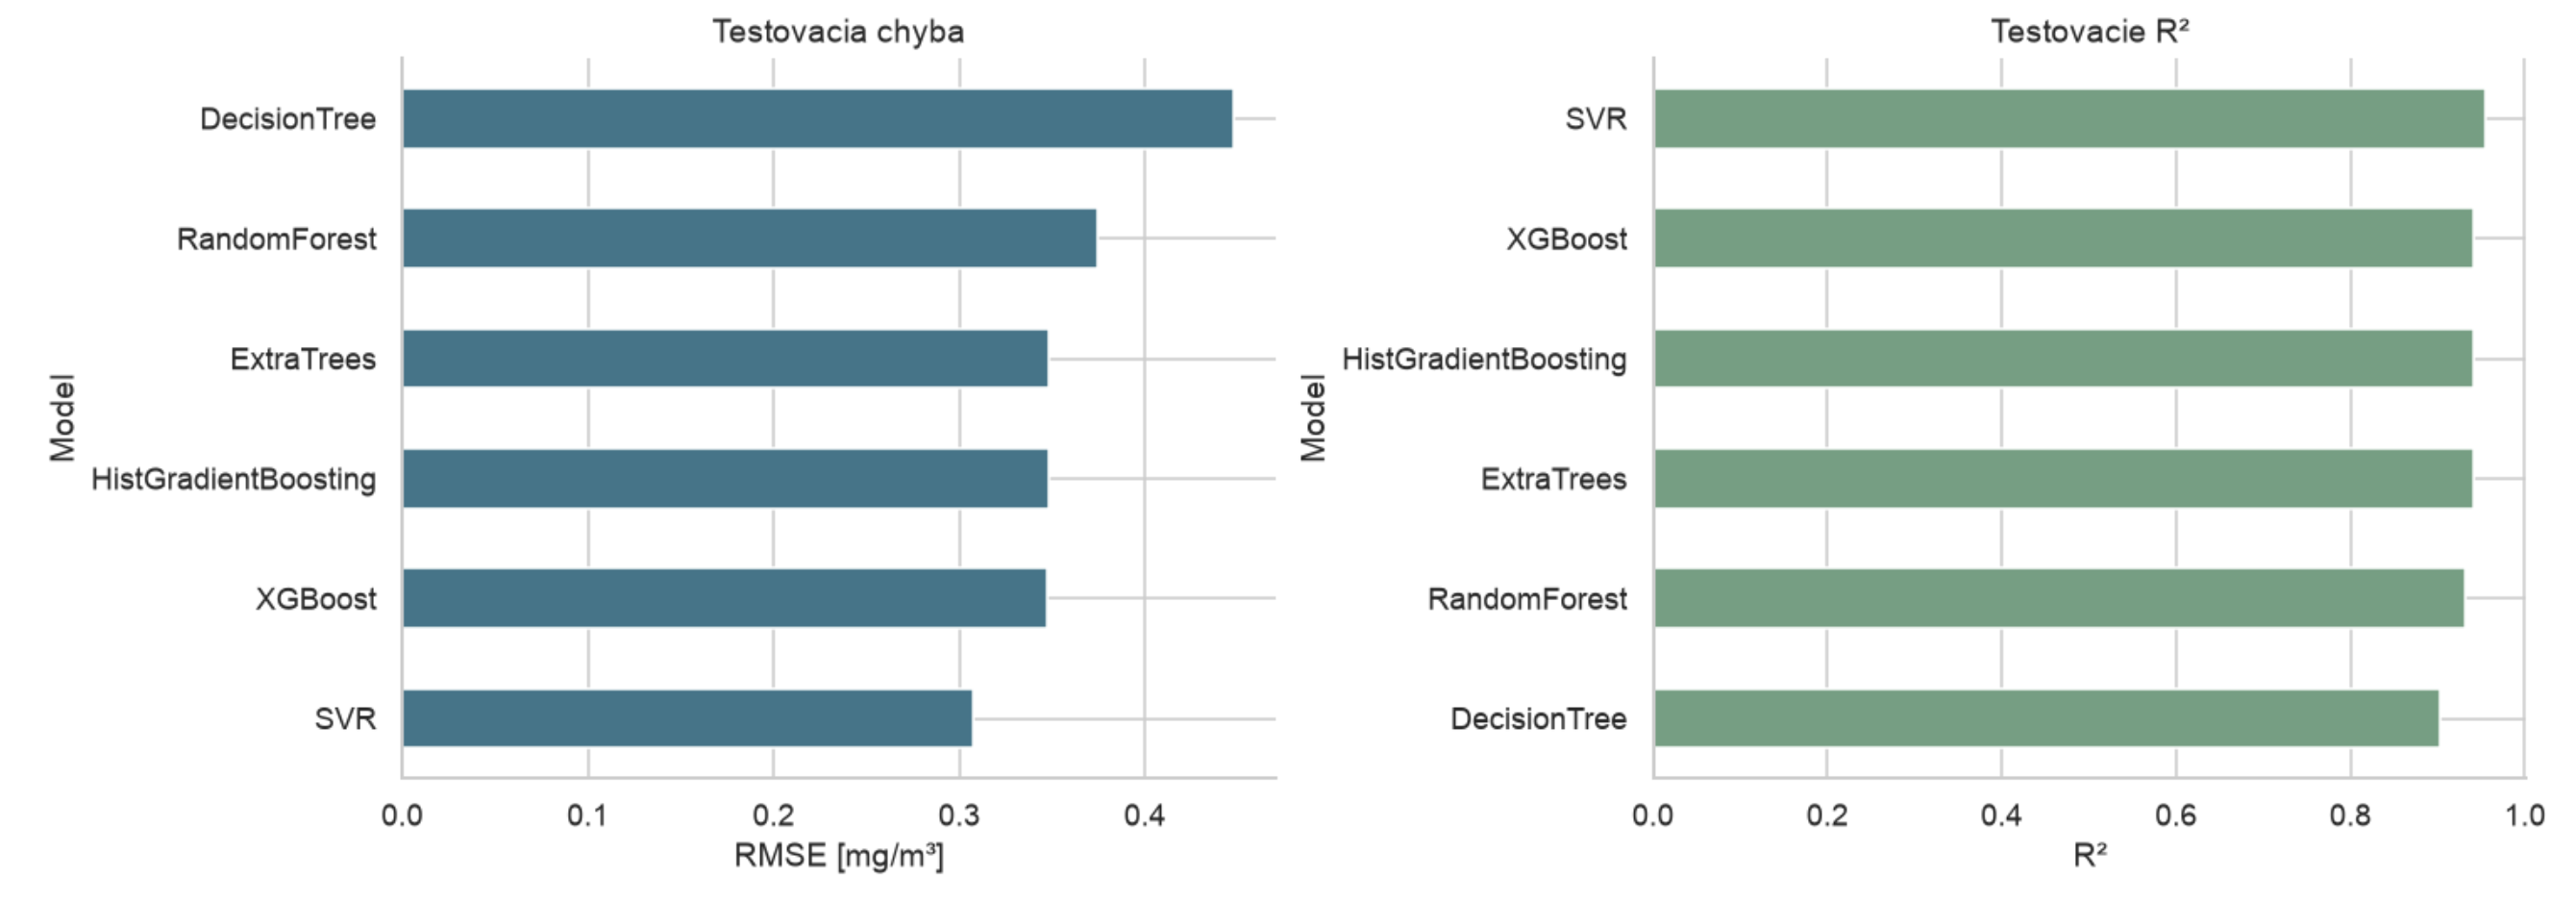
\includegraphics[width=\linewidth,keepaspectratio]{modely_porovnanie_metrik_graf.png}
\end{minipage}
\end{center}

% main.ipynb: bunka 105
CV víťaz \textbf{SVR} dosiahol na teste \textbf{\(R^2 = 0.9543\)}, \(\mathrm{RMSE} = \boldsymbol{0.3077\,\mathrm{mg}/\mathrm{m}^3}\).


% main.ipynb: bunka 111
Na zvislej osi bodových grafov je \textbf{reziduál} (skutočná hodnota - predikovaná hodnota). Ideálne body tvoria pás okolo nuly bez krivky či lievika. Histogram porovnáva chyby v tréningu a teste.

\begin{center}
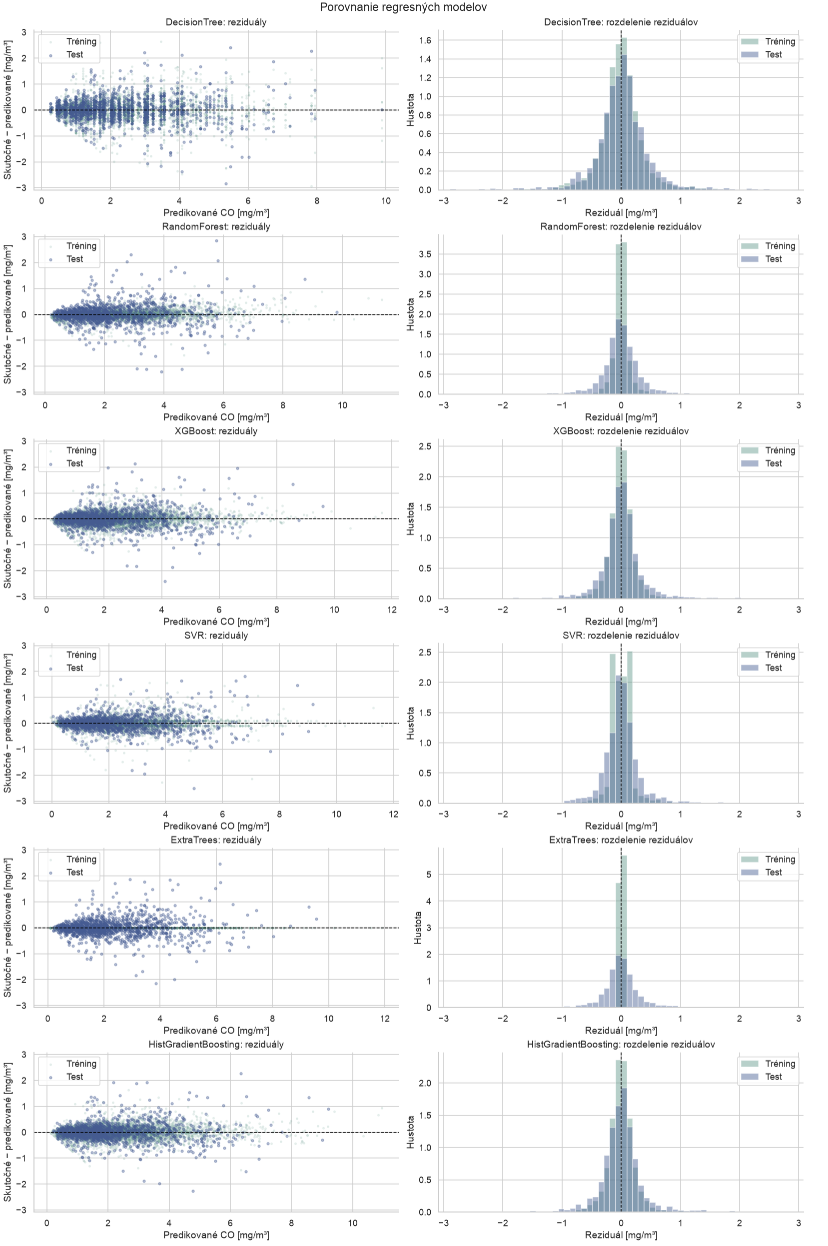
\includegraphics[width=0.84\linewidth,keepaspectratio,height=0.77\textheight]{modely_rezidualy_graf.png}
\end{center}

% main.ipynb: bunka 113
\textbf{SVR:} priemerný testovací reziduál 0.0019 \(\mathrm{mg}/\mathrm{m}^3\) znamená podhodnotenie v priemere. 95 \% absolútnych chýb neprekračuje \textbf{0.650 \(\mathrm{mg}/\mathrm{m}^3\)}. Korelácia veľkosti chyby s predikciou je 0.427. Chyby majú tendenciu rásť s predikovanou koncentráciou.


\subsubsection{Rozptyl reziduálov a chyby podľa skutočného CO}

\begin{center}
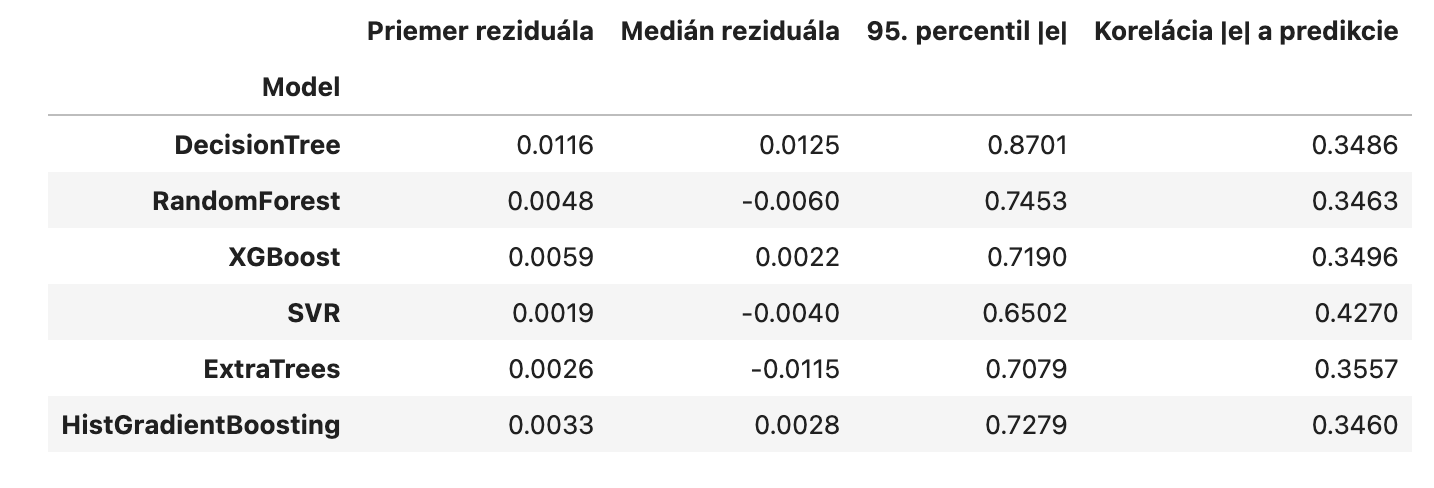
\includegraphics[width=\linewidth,keepaspectratio]{modely_rezidualy_tabulka.png}
\end{center}



% main.ipynb: bunka 114
Boxplot porovná rozdelenia testovacích reziduálov. Pásma CO určím podľa tréningových kvartilov. Testové merania ich nemenia. Pri každom pásme uvediem počet testovacích bodov.

\begin{center}
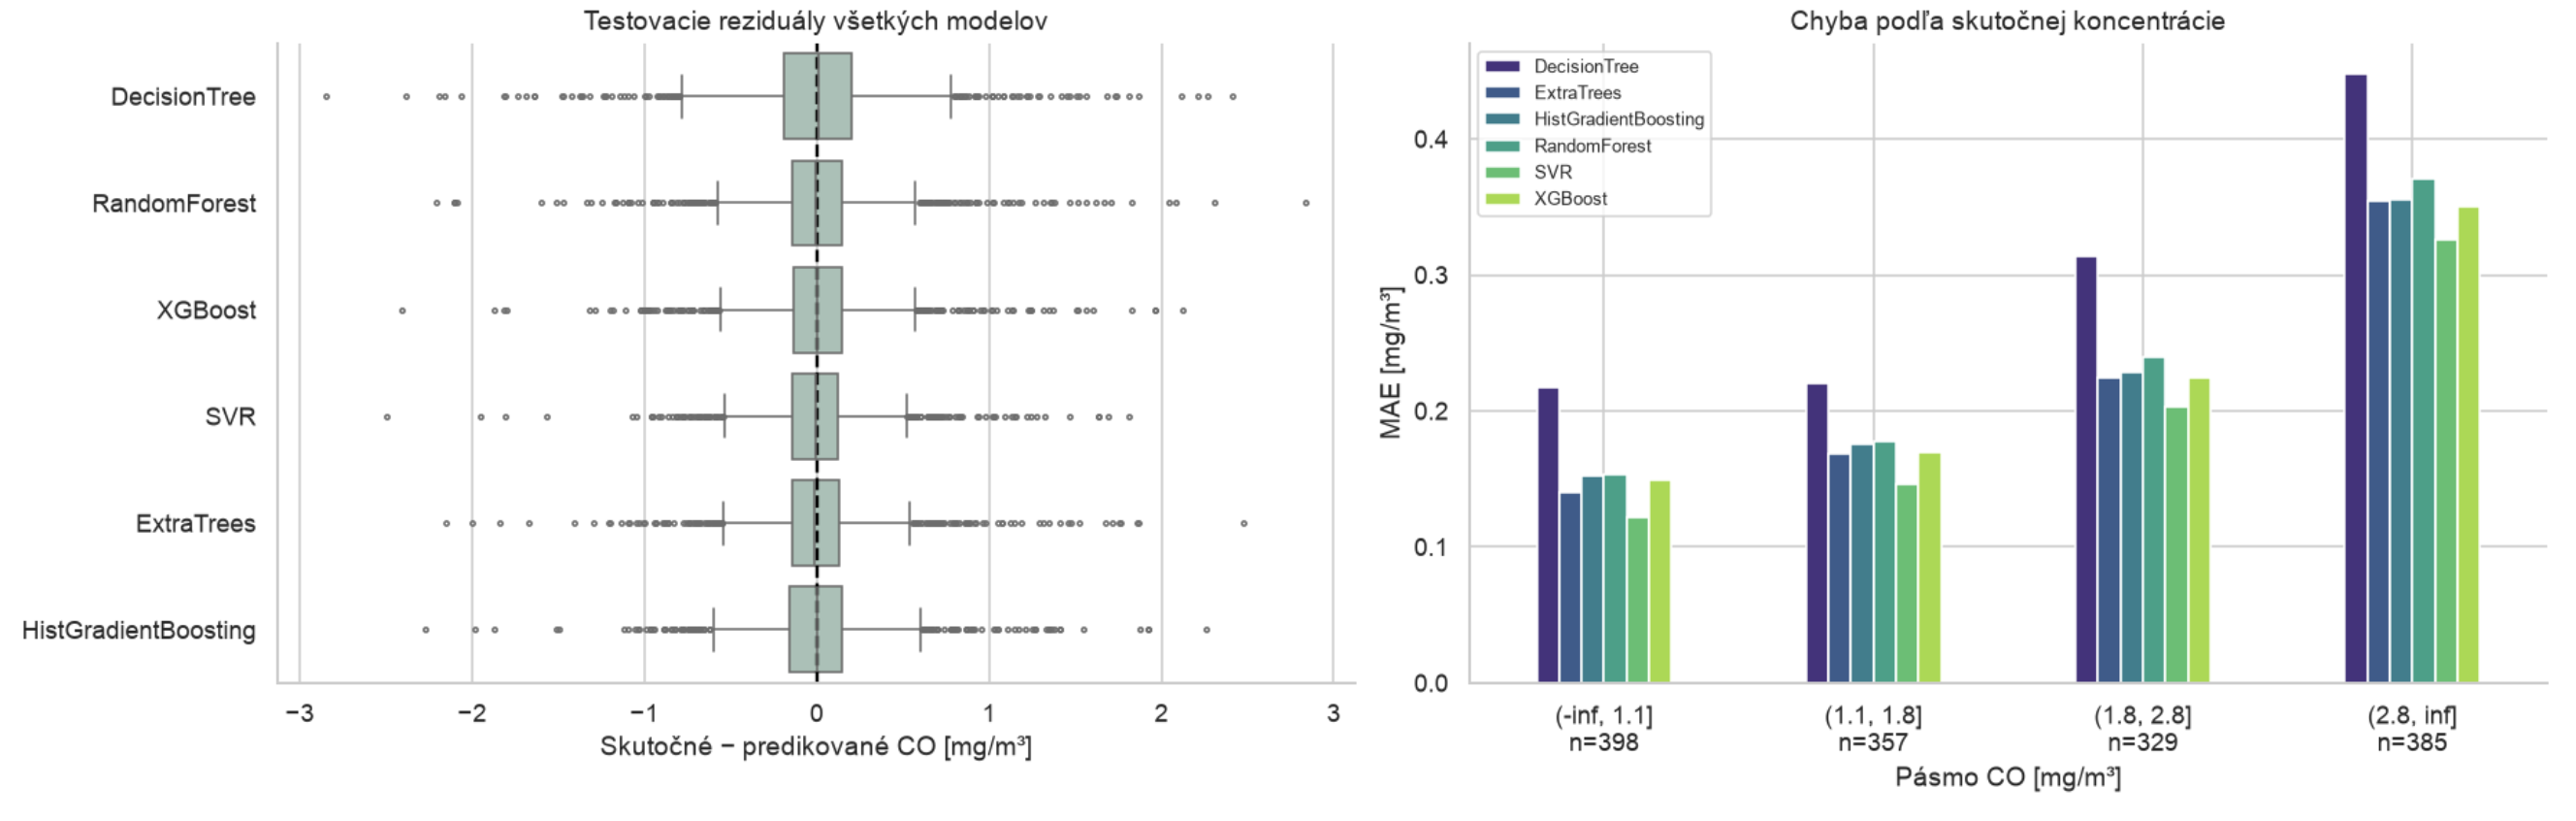
\includegraphics[width=\linewidth,keepaspectratio]{modely_rezidualy_a_chyby_podla_co_graf.png}
\end{center}

% main.ipynb: bunka 116
Pri modeli \textbf{SVR} je MAE v najnižšom pásme CO \textbf{0.1216 mg/m³}, v najvyššom \textbf{0.3256 mg/m³}. Najvyššie pásmo obsahuje \textbf{385} testovacích meraní a jeho priemerný reziduál je \textbf{0.0716 mg/m³}. Boxplot dopĺňa súhrnné metriky: posun mediánu ukazuje systematickú chybu, široký box a dlhé fúzy väčšie rozptýlenie reziduálov. Extrémne body ostávajú súčasťou hodnotenia.

\begin{center}
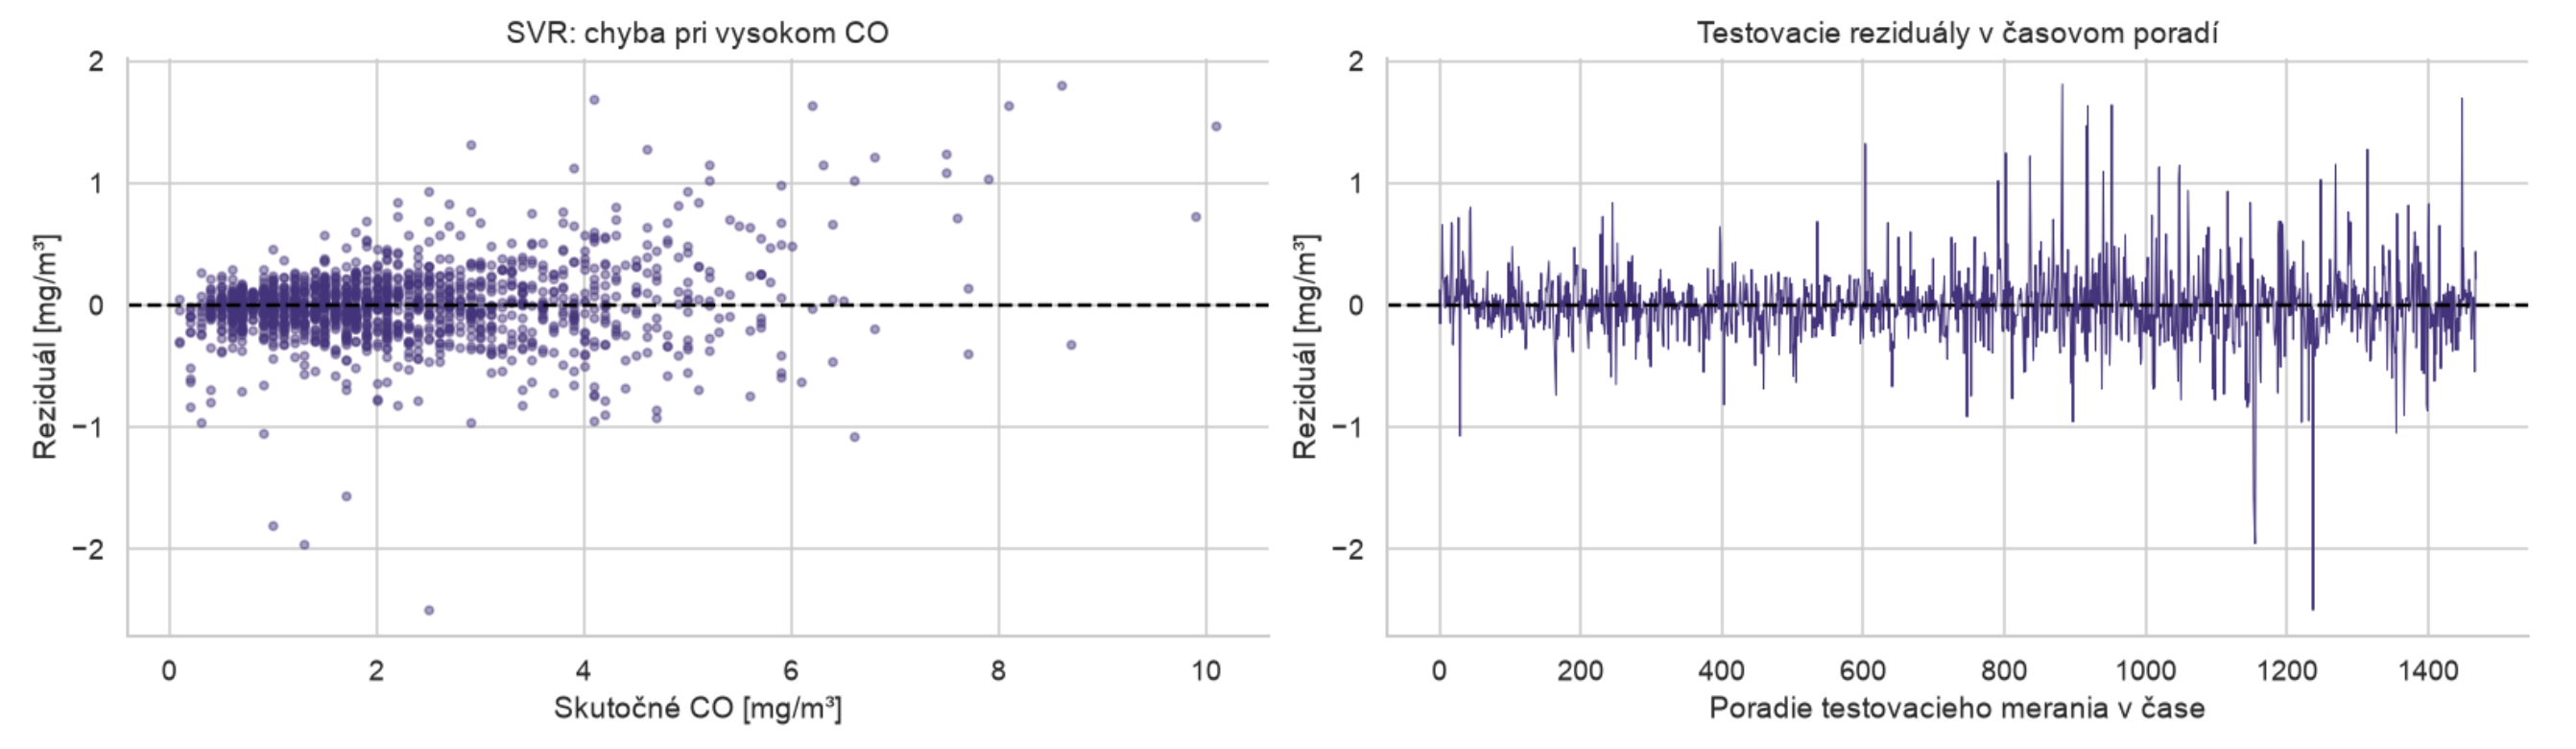
\includegraphics[width=\linewidth,keepaspectratio]{svr_rezidualy_podla_co_a_casu_graf.png}
\end{center}

% main.ipynb: bunka 118
Pri skutočnom CO aspoň \textbf{4.00 \(\mathrm{mg}/\mathrm{m}^3\)} (hranica z tréningu) je priemerný reziduál 0.137 \(\mathrm{mg}/\mathrm{m}^3\) na 182 testovacích bodoch. Tým priamo kontrolujem podhodnocovanie vysokých koncentrácií. Časový graf ukazuje poradie vybraných testovacích hodín. Vzdialenosť bodov na osi nie je rovnaký časový odstup. Nulový priemer reziduálov sám nezaručuje, že sú chyby nezávislé alebo normálne rozdelené.


% main.ipynb: bunka 119
\section{Redukcia dimenzie}

% main.ipynb: bunka 119
PCA vytvára nové osi ako lineárne kombinácie vstupov. PC1 zachytáva najväčší rozptyl, ďalšie kolmé osi zachytávajú zostávajúcu variabilitu. PCA nepozná cieľ CO, maximalizuje rozptyl vstupov, nie kvalitu regresie. Pred jej učením vstupy štandardizujem, pretože samotná PCA ich iba centruje.

% main.ipynb: bunka 119
\subsection{Vykreslenie príznakov -- vyčítanie závislostí}

% main.ipynb: bunka 119
Vyberám \texttt{sensor\_\allowbreak{}co}, \texttt{sensor\_\allowbreak{}nmhc} a \texttt{sensor\_\allowbreak{}nox}. Použijem rovnakú podvzorku najviac 2 500 tréningových inlierov.

\begin{center}
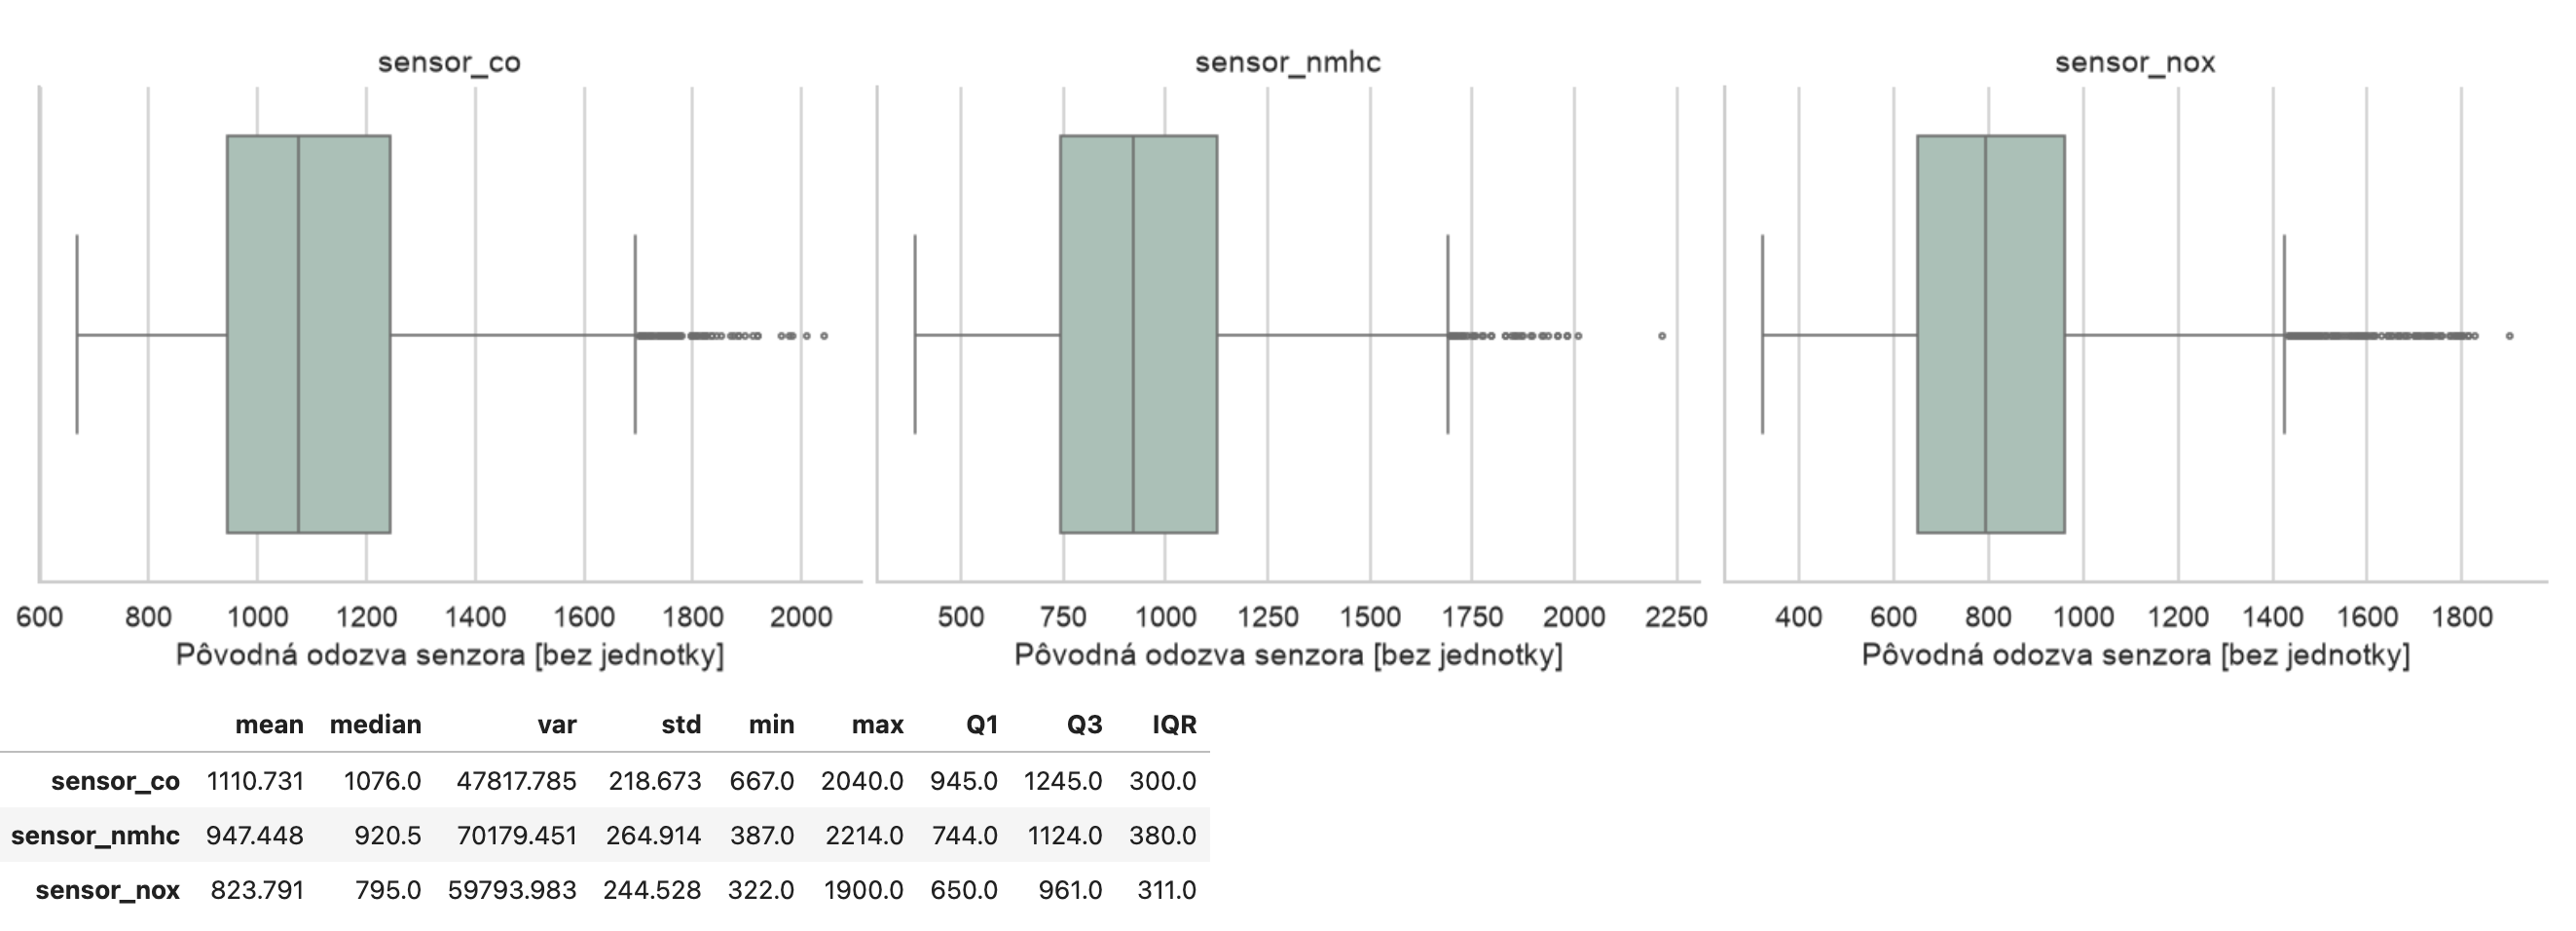
\includegraphics[width=\linewidth,keepaspectratio]{pca_povodne_senzory_boxploty_a_statistika.png}
\end{center}

% main.ipynb: bunka 122
\subsection{Minimalizácia na 3 dimenzie}

% main.ipynb: bunka 122
Kódovanie, štandardizáciu a PCA učím iba na tréningových inlieroch. Transformácia prevádza 17 vstupných stĺpcov na PC1, PC2 a PC3. Rovnaké parametre následne transformujú test.

\begin{center}
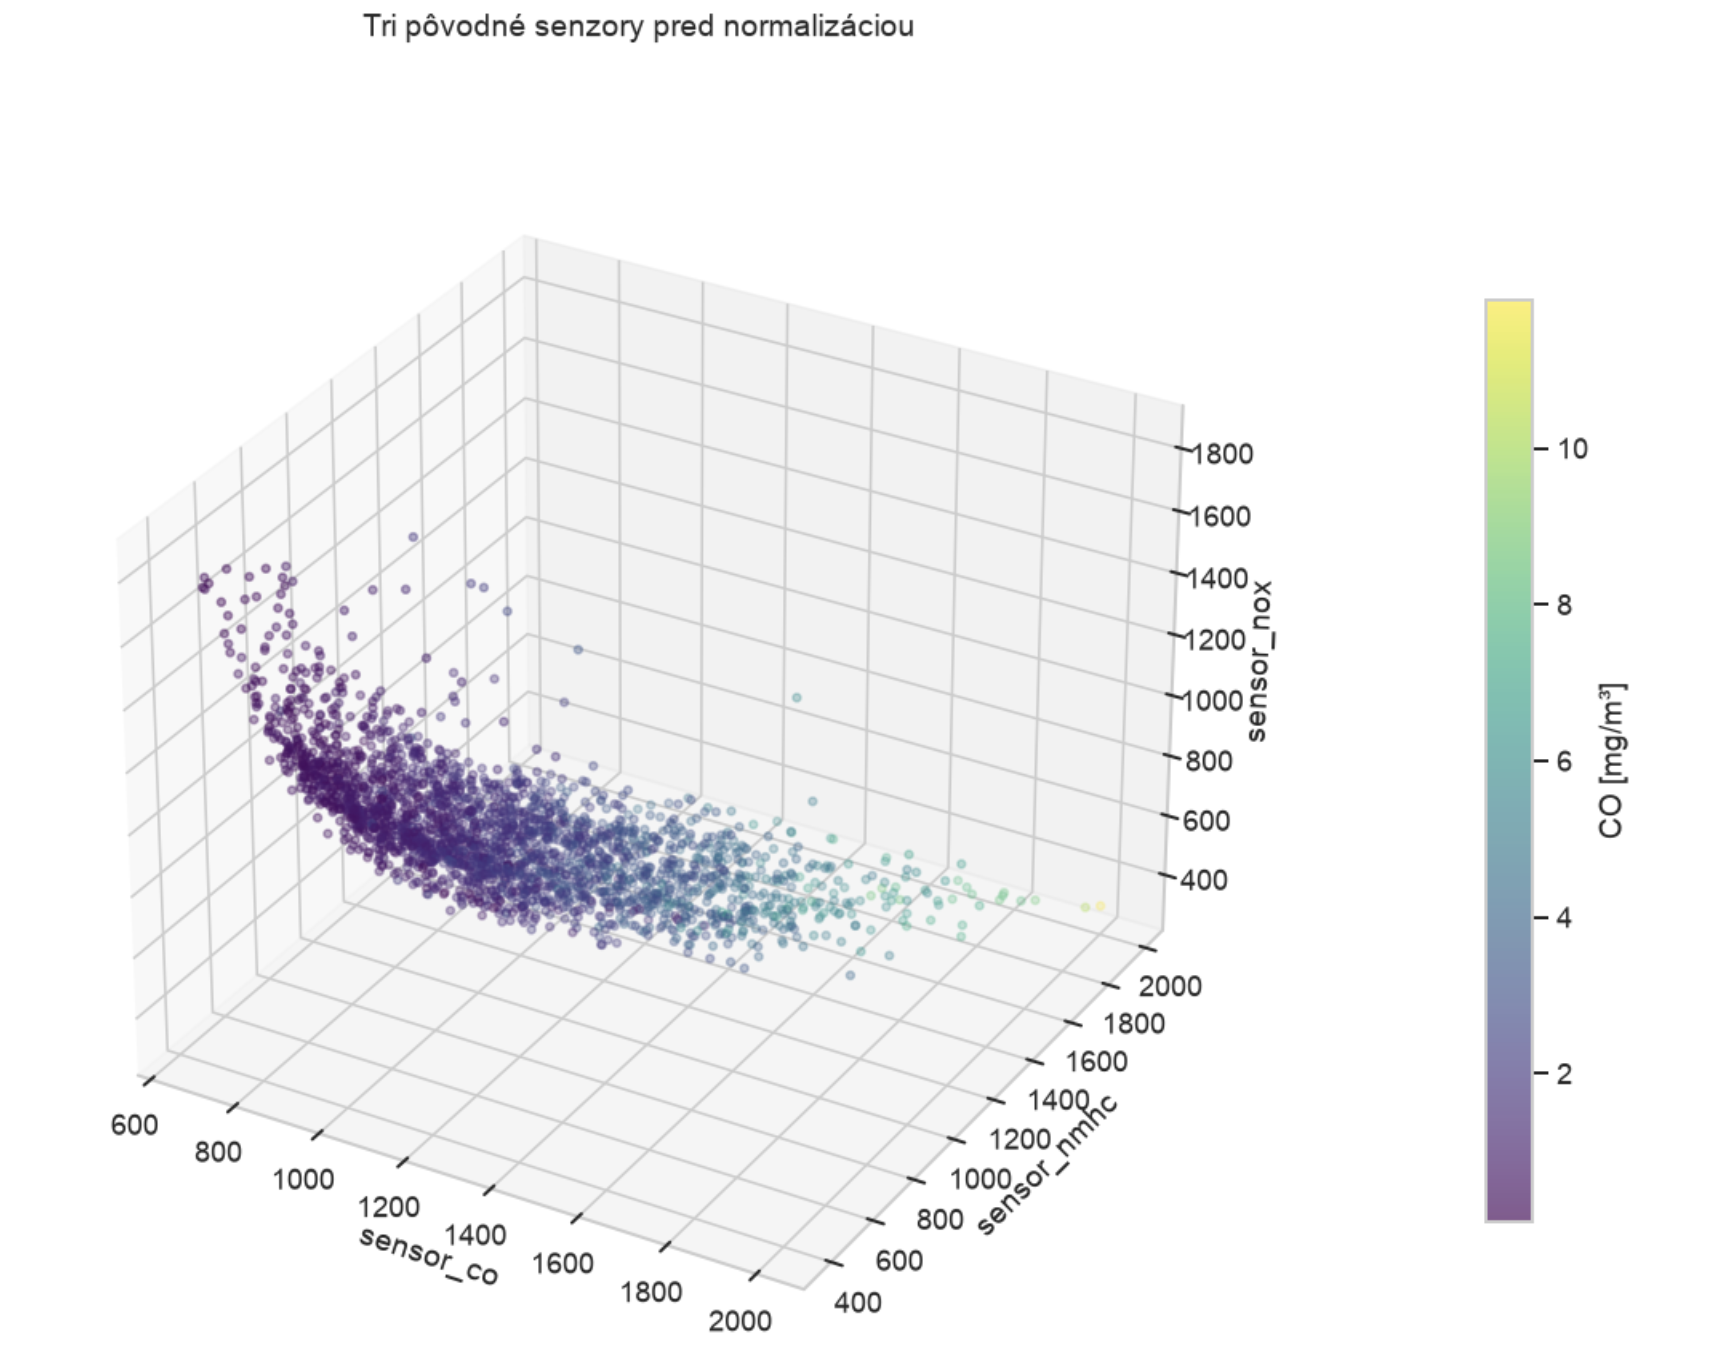
\includegraphics[width=0.49\linewidth,keepaspectratio]{pca_povodne_senzory_3d_graf.png}\hfill
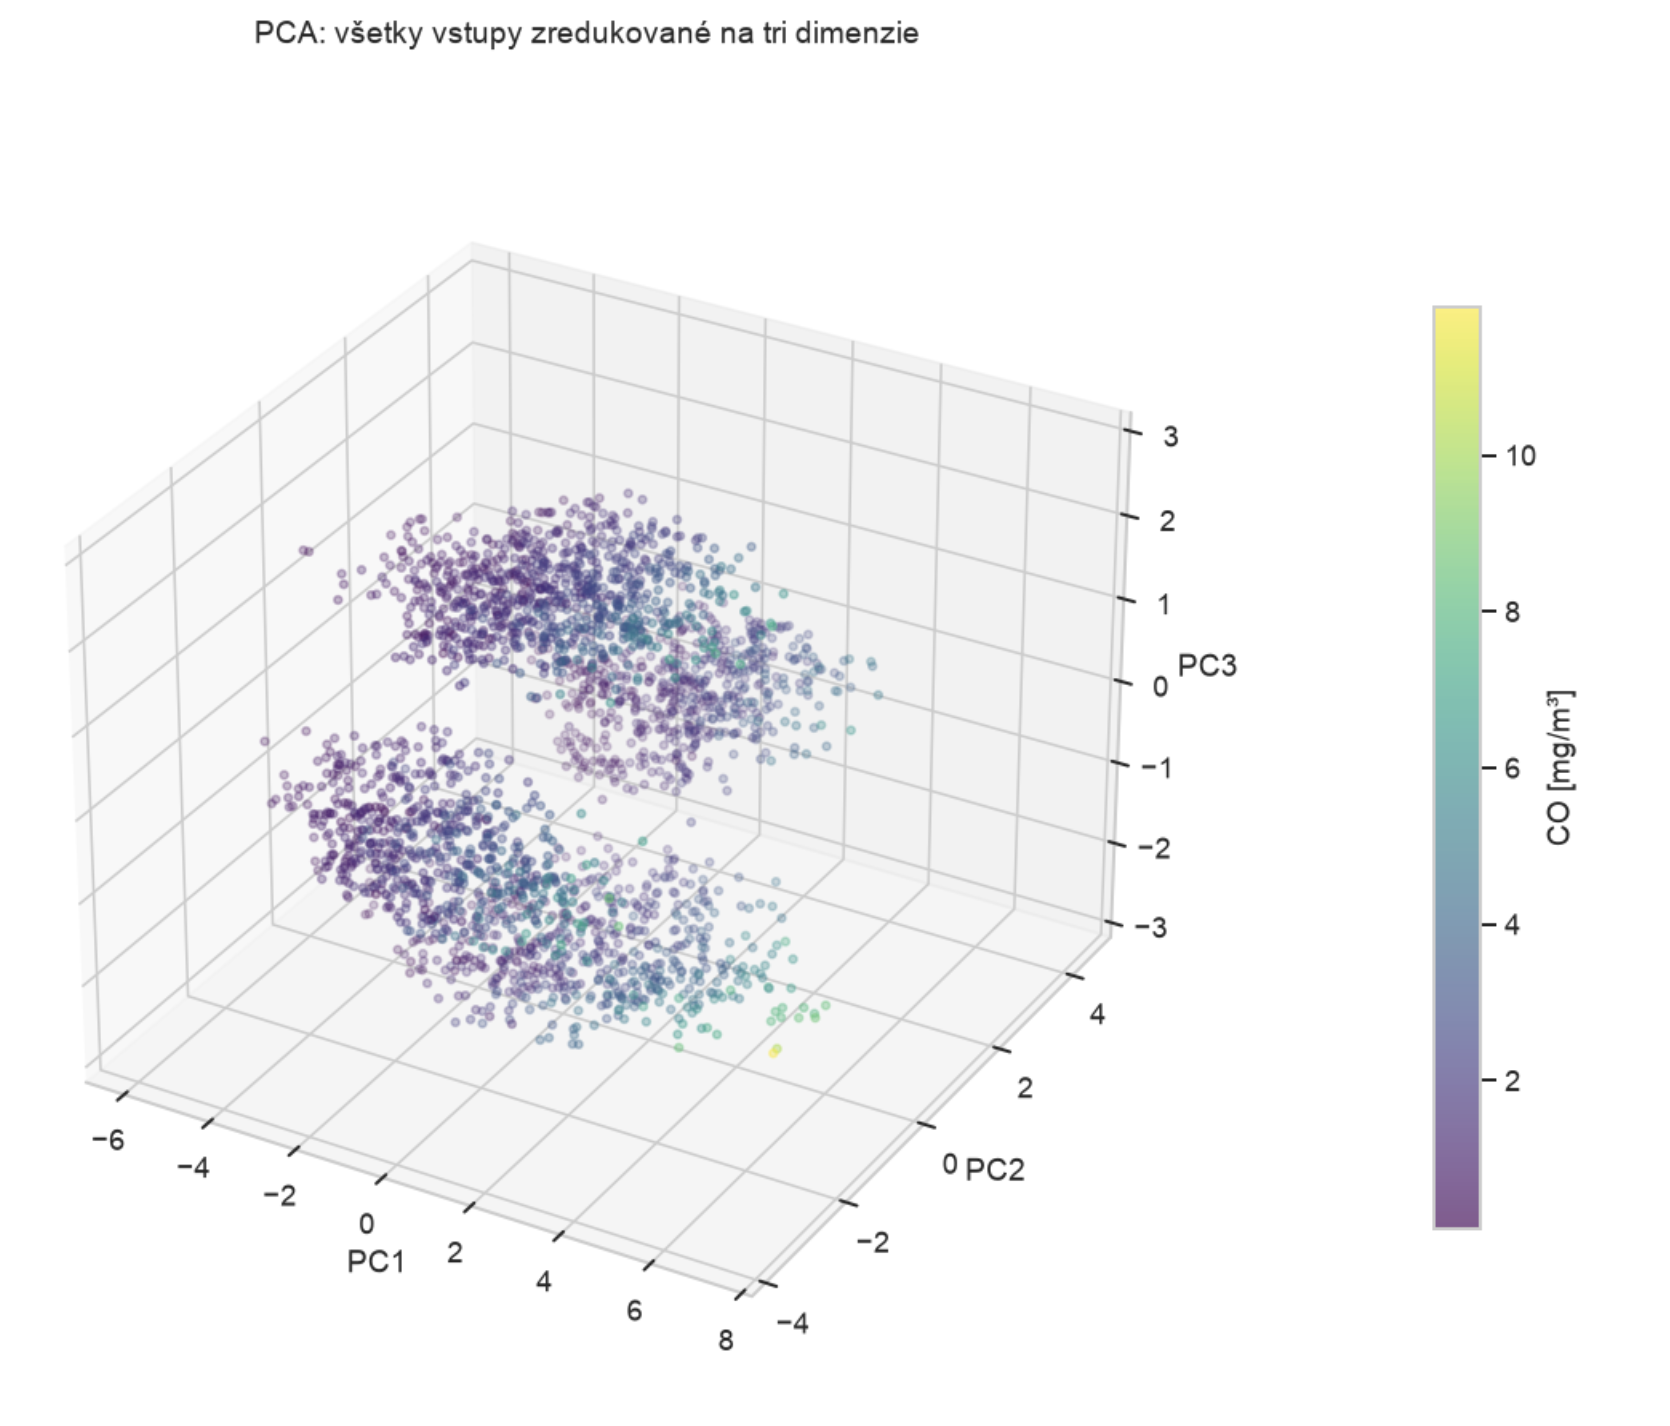
\includegraphics[width=0.49\linewidth,keepaspectratio]{pca_projekcia_3d_graf.png}
\end{center}

% main.ipynb: bunka 124
Tri komponenty zachovávajú \textbf{60.2\% vstupnej variability} (jednotlivo 26.0\%, 20.4\%, 13.8\%). Korelácie PC1, PC2 a PC3 s CO sú 0.848, -0.310, 0.068. V pôvodnom grafe sú vyššie koncentrácie sústredené pri vyšších odozvách sensor\_co a sensor\_nmhc a pri nižších odozvách sensor\_nox. Farebný prechod teda odhaľuje súvislosť viacerých senzorov s CO. V PCA sa hlavný farebný gradient orientuje najmä pozdĺž PC1, čo podporuje aj jeho korelácia s CO.

% main.ipynb: bunka 135
Tri PC zachovávajú približne \textbf{60,22 \%} vstupného rozptylu, zvyšných \textbf{39,78 \%} tento obrázok nezobrazuje. Viditeľné pásy nie sú triedy CO. Ani čitateľnejší obraz sám nepreukazuje lepšiu regresiu.

\begin{center}
\noindent
\begin{minipage}[c]{0.6\linewidth}
\centering
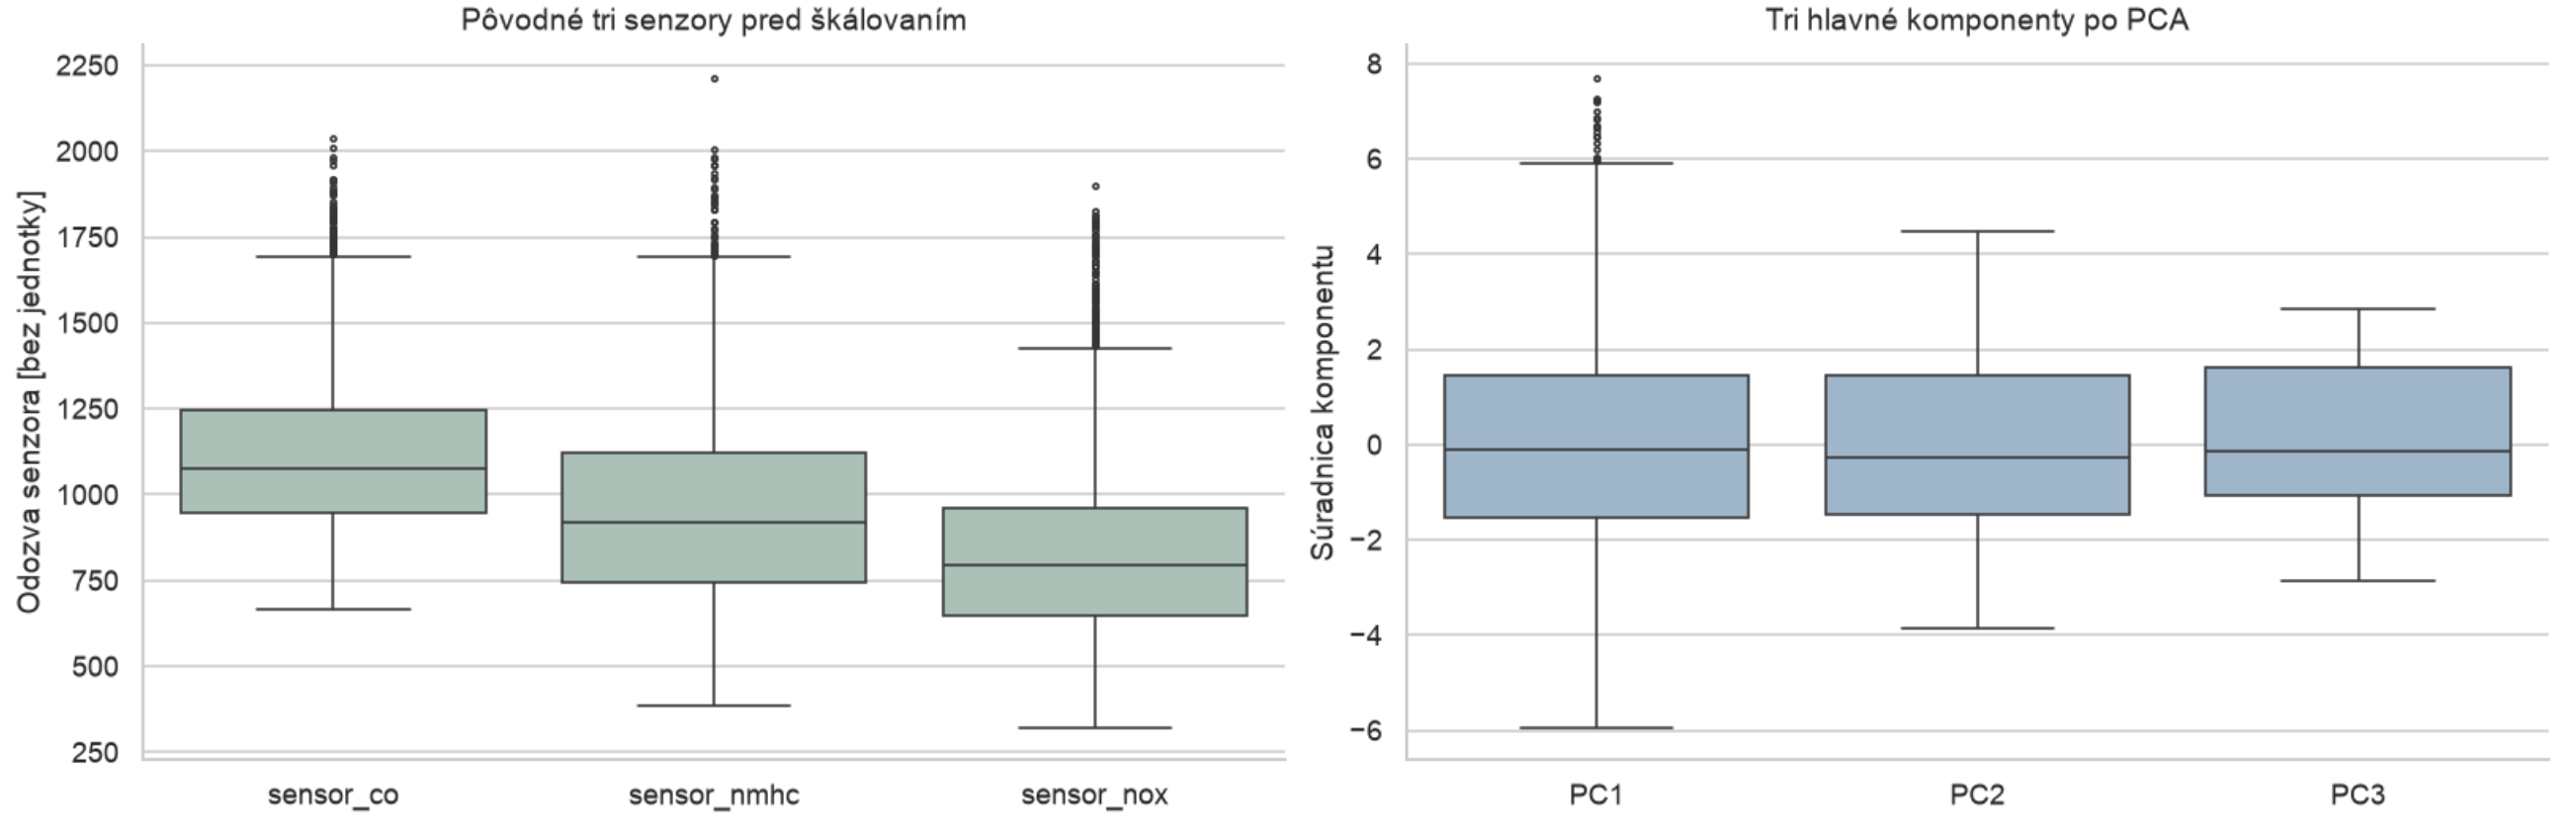
\includegraphics[width=\linewidth,keepaspectratio]{pca_senzory_a_komponenty_boxploty.png}
\end{minipage}\hfill%
\begin{minipage}[c]{0.37\linewidth}
\centering
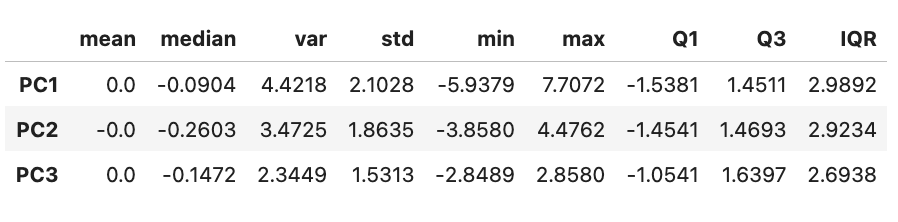
\includegraphics[width=\linewidth,keepaspectratio]{pca_statistika_komponentov_tabulka.png}
\end{minipage}
\end{center}

Vľavo sú tri vybrané pôvodné senzory, komponenty však vznikli zo všetkých 17 štandardizovaných vstupov. Ich súradnice majú inú mierku než pôvodné odozvy senzorov.

% \subsection{Interpretácia hlavných komponentov}

% Heatmapa zobrazuje koeficienty všetkých 17 vstupov so znamienkom. Tabuľka dopĺňa absolútne hodnoty koeficientov ôsmich vybraných vstupov. Nejde o dôležitosť príznakov regresného modelu ani o koreláciu s CO.

% \begin{center}
% \noindent
% \begin{minipage}[c]{0.64\linewidth}
% \centering
% 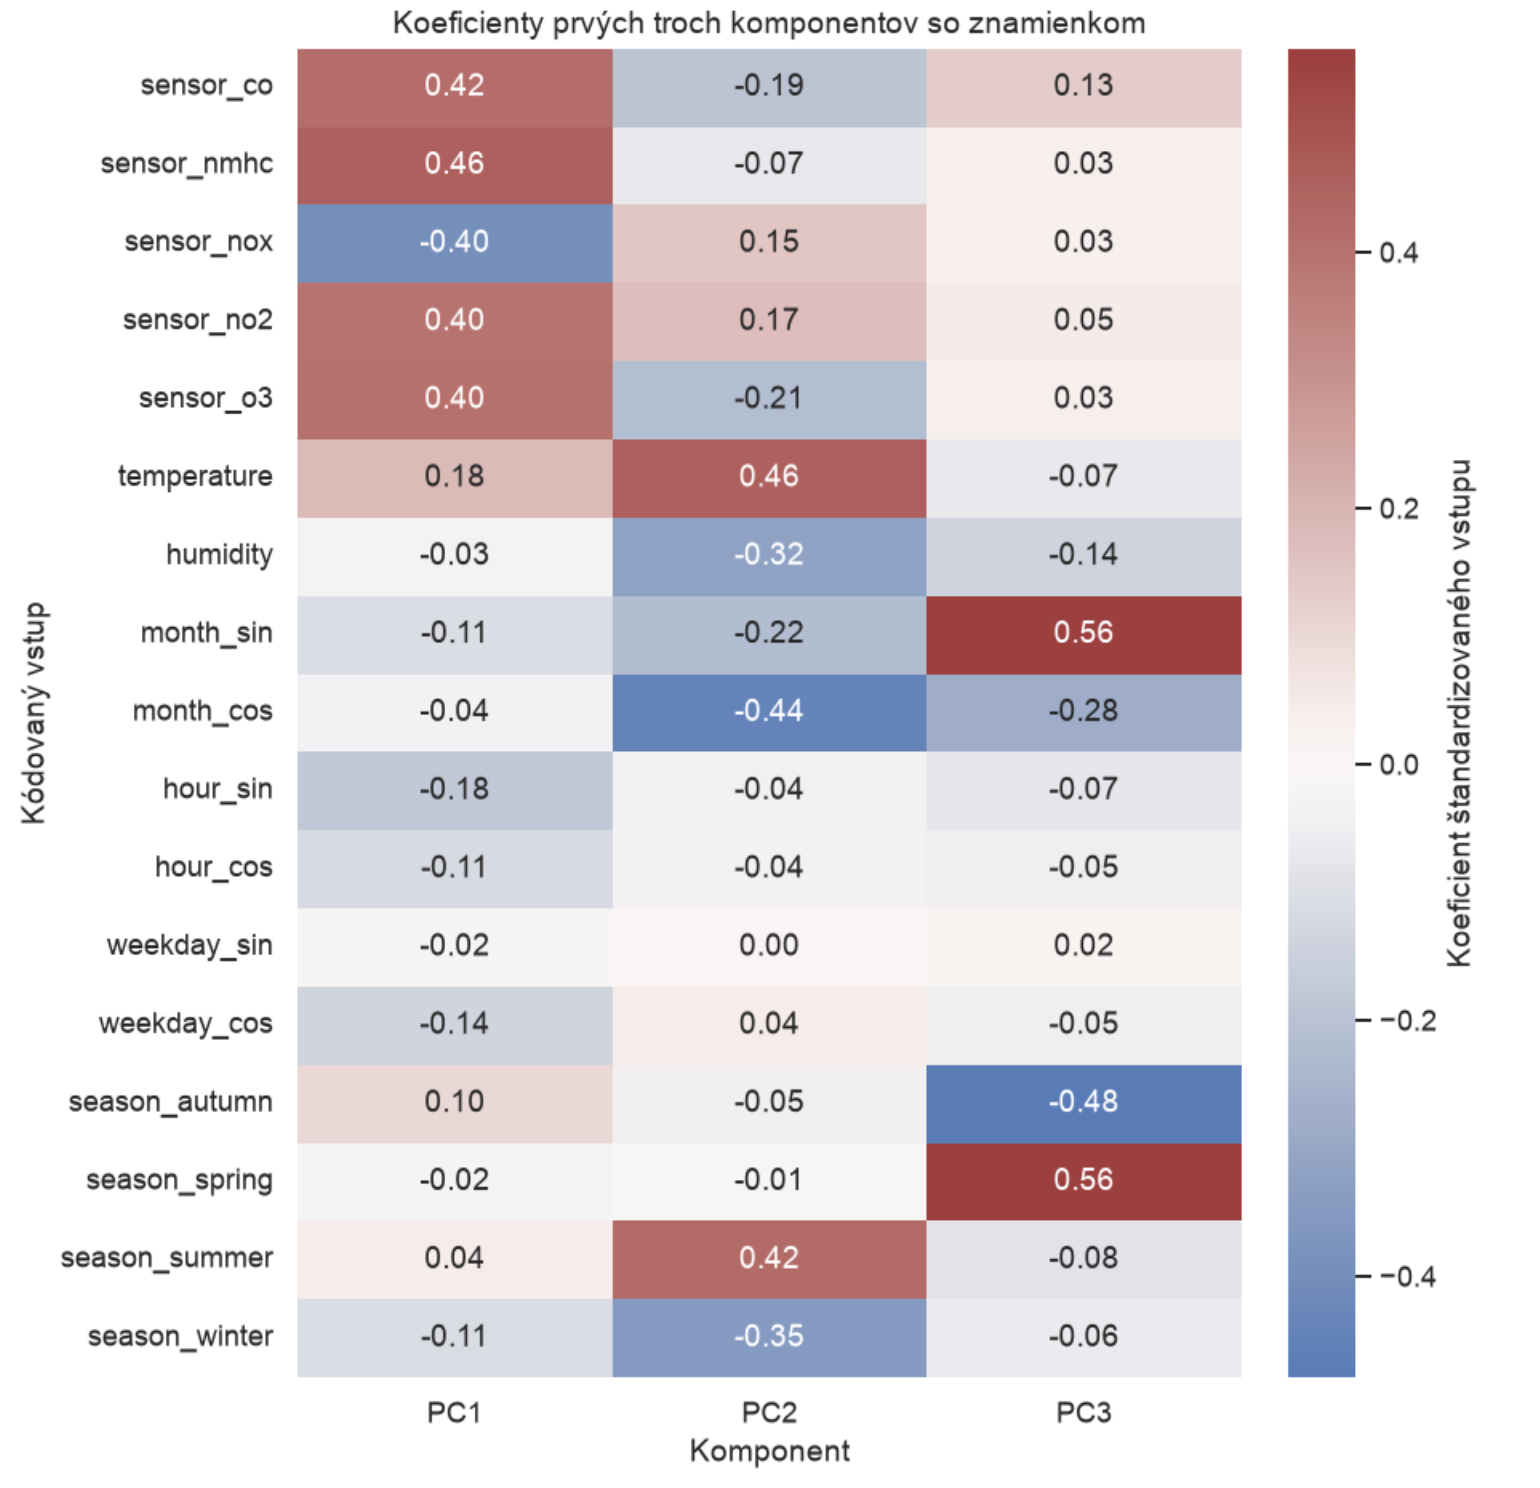
\includegraphics[width=\linewidth,keepaspectratio]{pca_koeficienty_heatmapa.png}
% \end{minipage}\hfill%
% \begin{minipage}[c]{0.33\linewidth}
% \centering
% 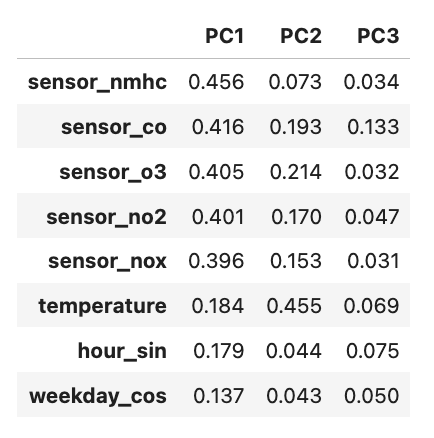
\includegraphics[width=\linewidth,keepaspectratio]{pca_absolutne_koeficienty_tabulka.png}
% \end{minipage}
% \end{center}

% PC1 spája najmä odozvy senzorov: kladné koeficienty majú napríklad \texttt{sensor\_nmhc} a \texttt{sensor\_co}, záporný \texttt{sensor\_nox}. PC2 výraznejšie zahŕňa teplotu a sezónne premenné, PC3 najmä \texttt{month\_sin} a jarnú sezónu. Globálne obrátenie znamienka komponentu nemení jeho vysvetlený rozptyl.


% main.ipynb: bunka 136
\section{Trénovanie modelu na zmenšenej množine}

% main.ipynb: bunka 136
Používam rovnaký typ a hyperparametre modelu vybraného v prvej časti podľa CV. Počet ponechaných príznakov alebo prah PCA vyberám vo vnútri tréningovej CV. Každý selector sa učí iba na tréningovej časti daného foldu. Test zostáva spoločný pre všetky stratégie.

% main.ipynb: bunka 139
\subsection{Korelačná matica}

% main.ipynb: bunka 139
Zoradím vstupy podľa absolútnej Pearsonovej korelácie s CO a vynechám príznaky s absolútnou koreláciou aspoň 0,95 s už vybraným vstupom. CV vyberá najviac 4 alebo 8 príznakov. Heatmapa nižšie je opis finálneho tréningového výberu, nie podklad na výber podľa testu.

\begin{center}
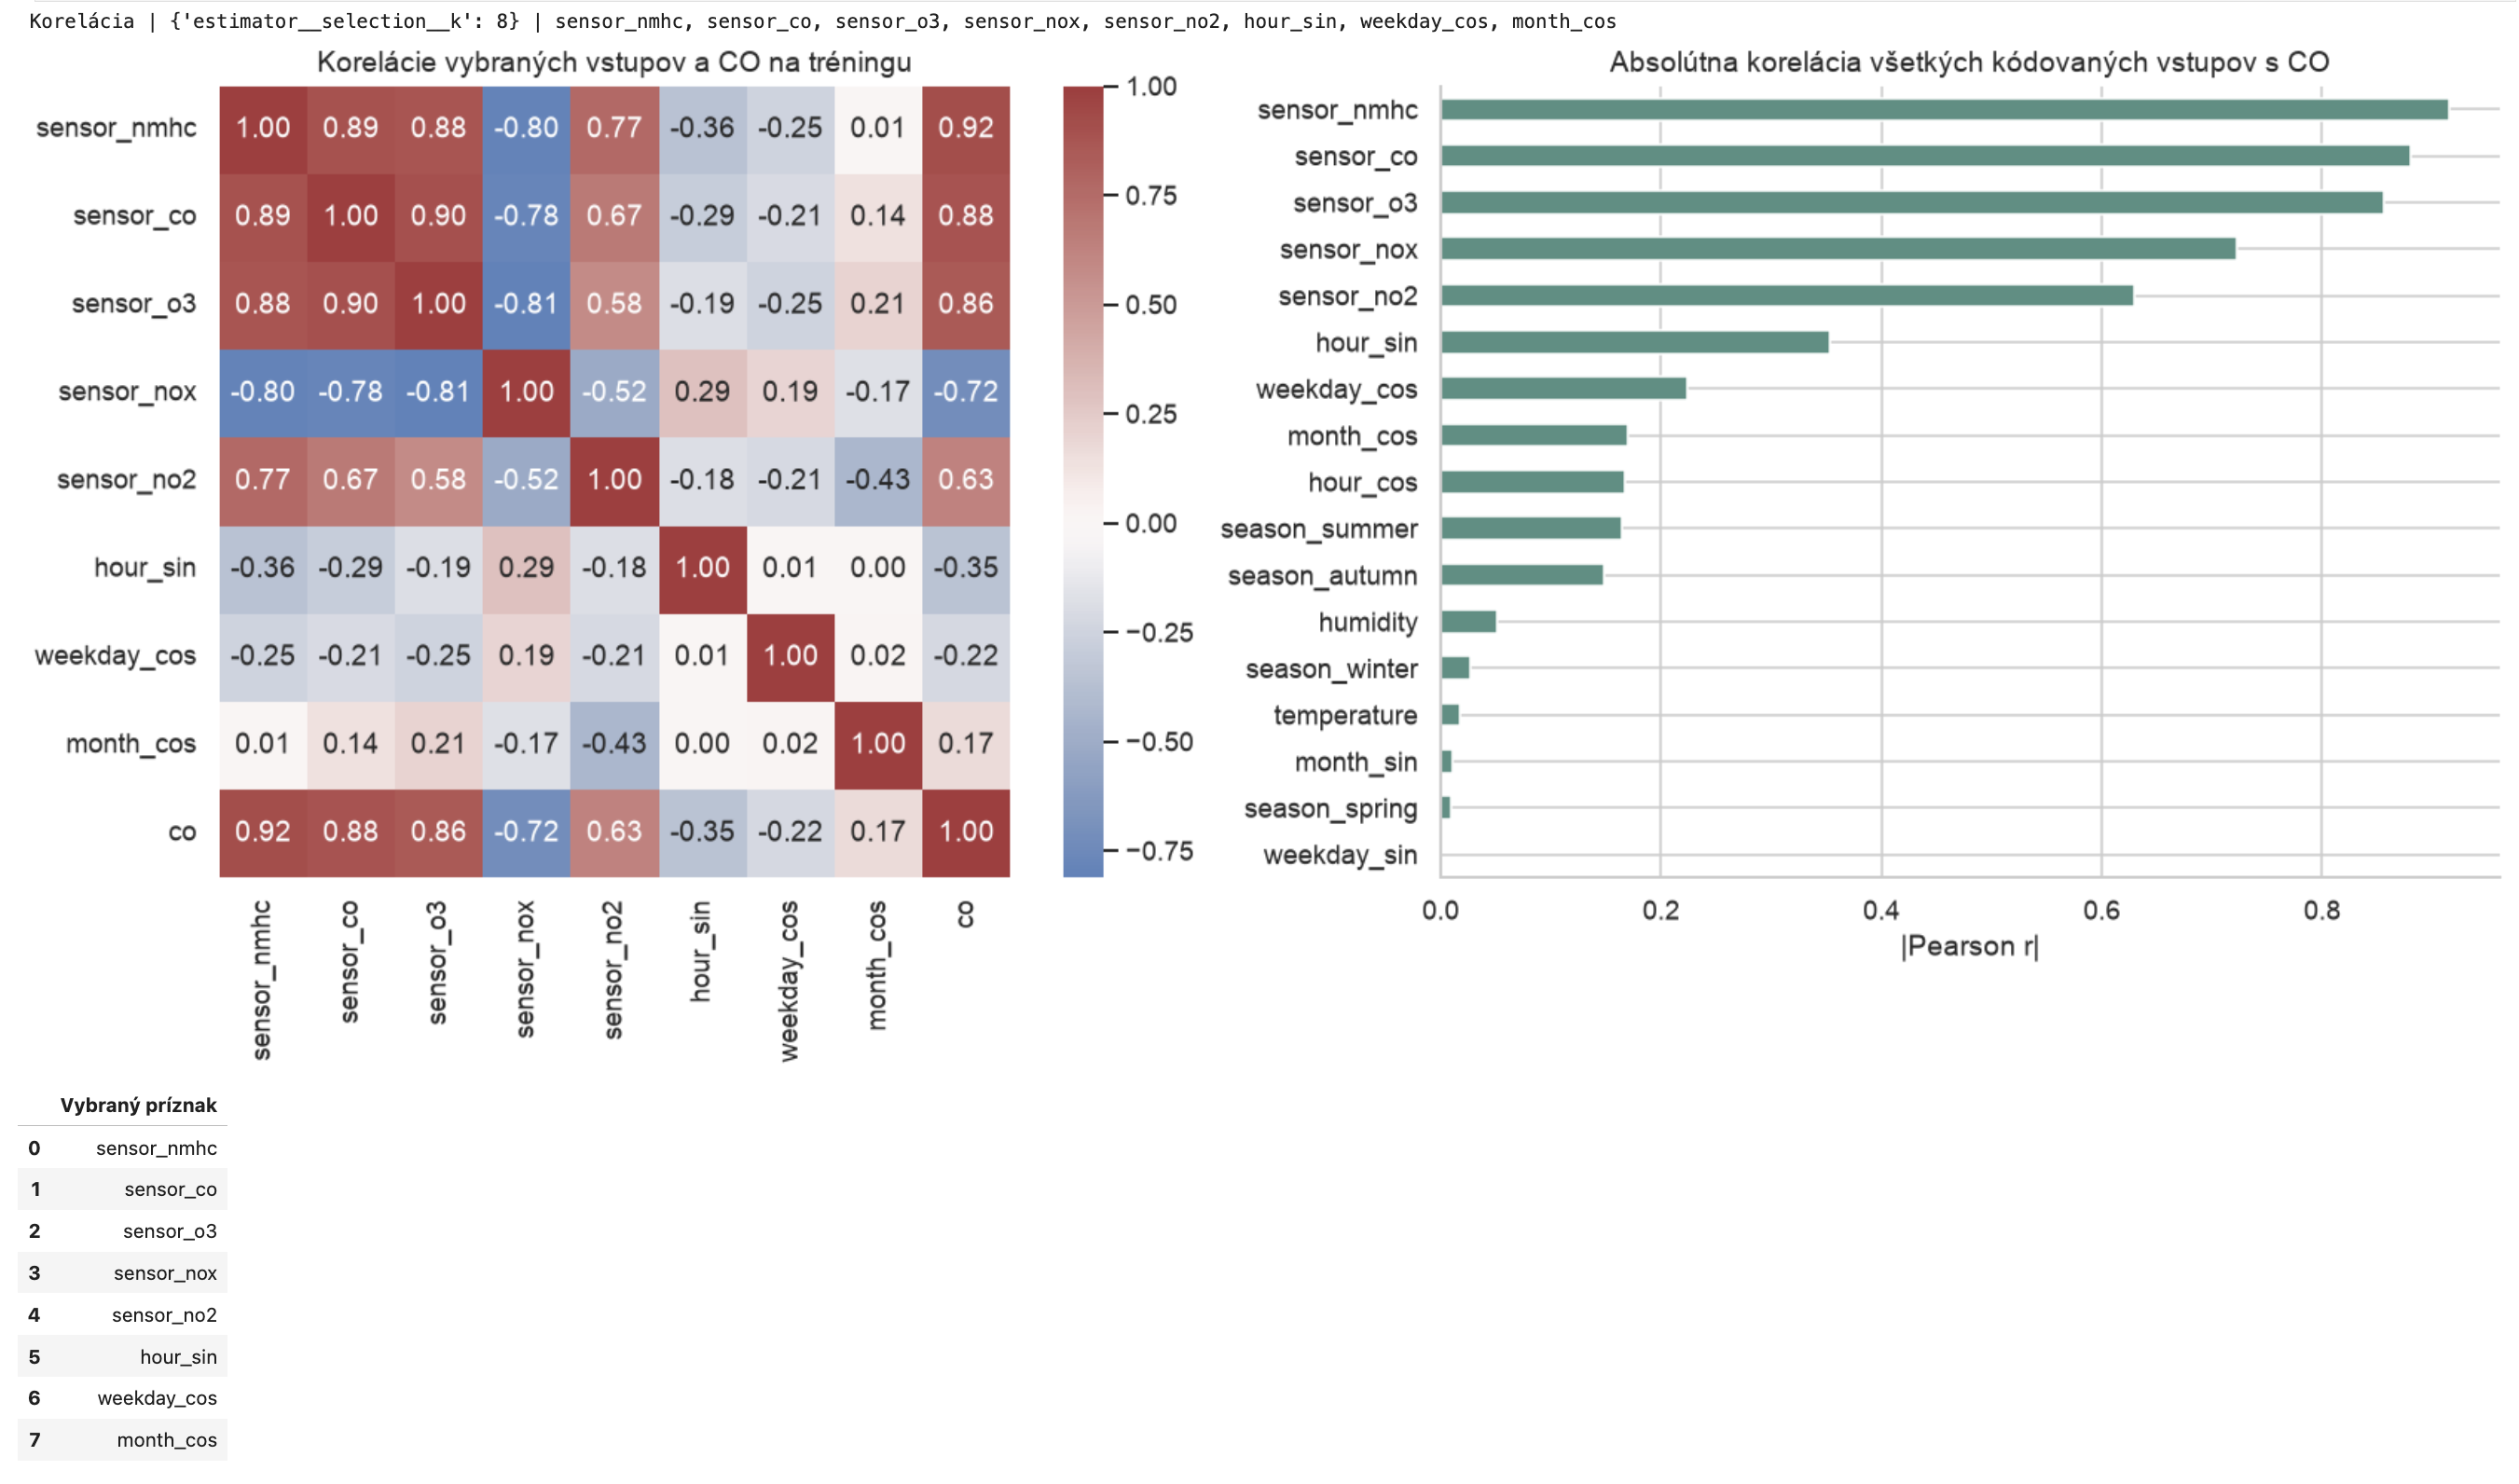
\includegraphics[width=\linewidth,keepaspectratio,height=0.26\textheight]{redukcia_vyber_podla_korelacie_graf.png}
\end{center}

% main.ipynb: bunka 141
\textbf{Korelácia:} 8 vstupov, testovacie \(R^2\) \textbf{0.9248}, RMSE \textbf{0.3946 \(\mathrm{mg}/\mathrm{m}^3\)}, rozdiel RMSE oproti plnému modelu +0.0869 \(\mathrm{mg}/\mathrm{m}^3\).

% main.ipynb: bunka 142
\subsection{Dôležitosť príznakov z ensemble}

% main.ipynb: bunka 142
Pomocný Random Forest sa v každom CV folde učí od začiatku a podľa jeho natívnych dôležitostí vyberám 4 alebo 8 príznakov. Na vybraných príznakoch následne od začiatku trénujem SVR s pôvodnými hyperparametrami, počet príznakov volím podľa jeho CV MSE.

\begin{center}
\noindent
\begin{minipage}[c]{0.70\linewidth}
\centering
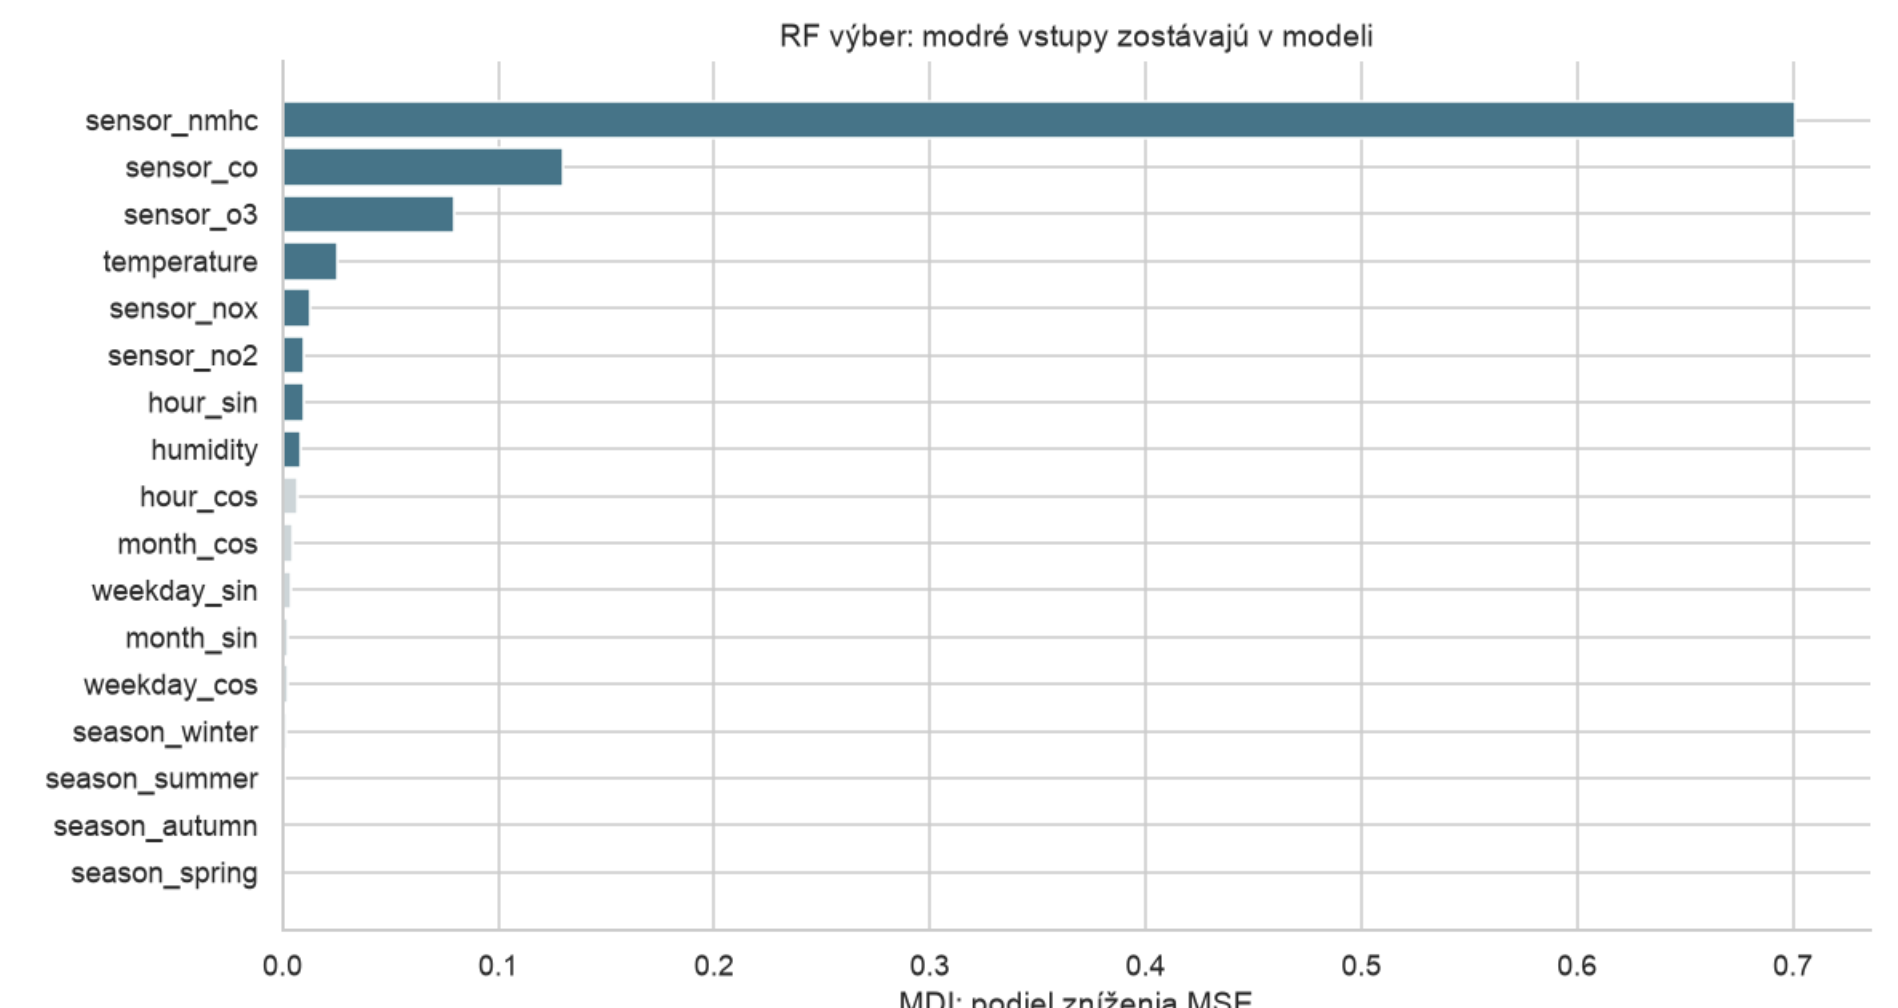
\includegraphics[width=\linewidth,keepaspectratio]{redukcia_vyber_podla_rf_graf.png}
\end{minipage}\hfill%
\begin{minipage}[c]{0.27\linewidth}
\centering
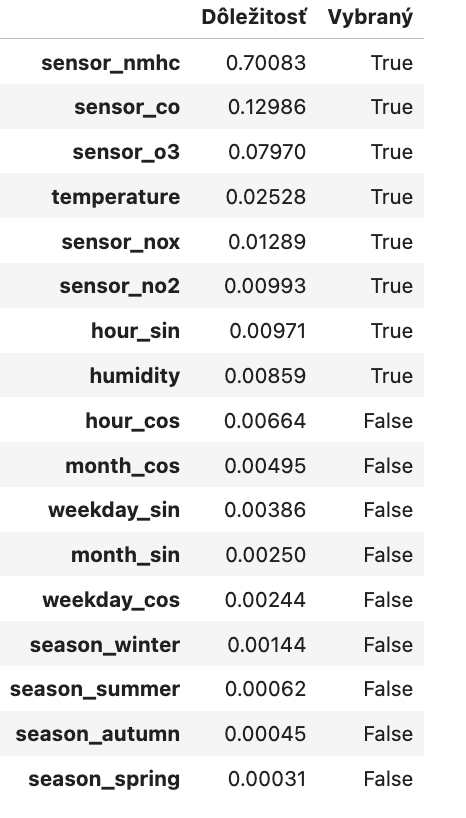
\includegraphics[width=\linewidth,keepaspectratio]{redukcia_vyber_podla_rf_tabulka.png}
\end{minipage}
\end{center}

% main.ipynb: bunka 144
\textbf{RF dôležitosť:} 8 vstupov, testovacie \(R^2\) \textbf{0.9314}, RMSE \textbf{0.3770 \(\mathrm{mg}/\mathrm{m}^3\)}, rozdiel RMSE oproti plnému modelu +0.0693 \(\mathrm{mg}/\mathrm{m}^3\).

% main.ipynb: bunka 145
\subsection{Podľa variancie}

% main.ipynb: bunka 145
PCA skúša hranice vysvetlenej variability 90 \%, 95 \% a 99 \%. Počet komponentov vyplynie z dát.

\begin{center}
\noindent
\begin{minipage}[c]{0.64\linewidth}
\centering
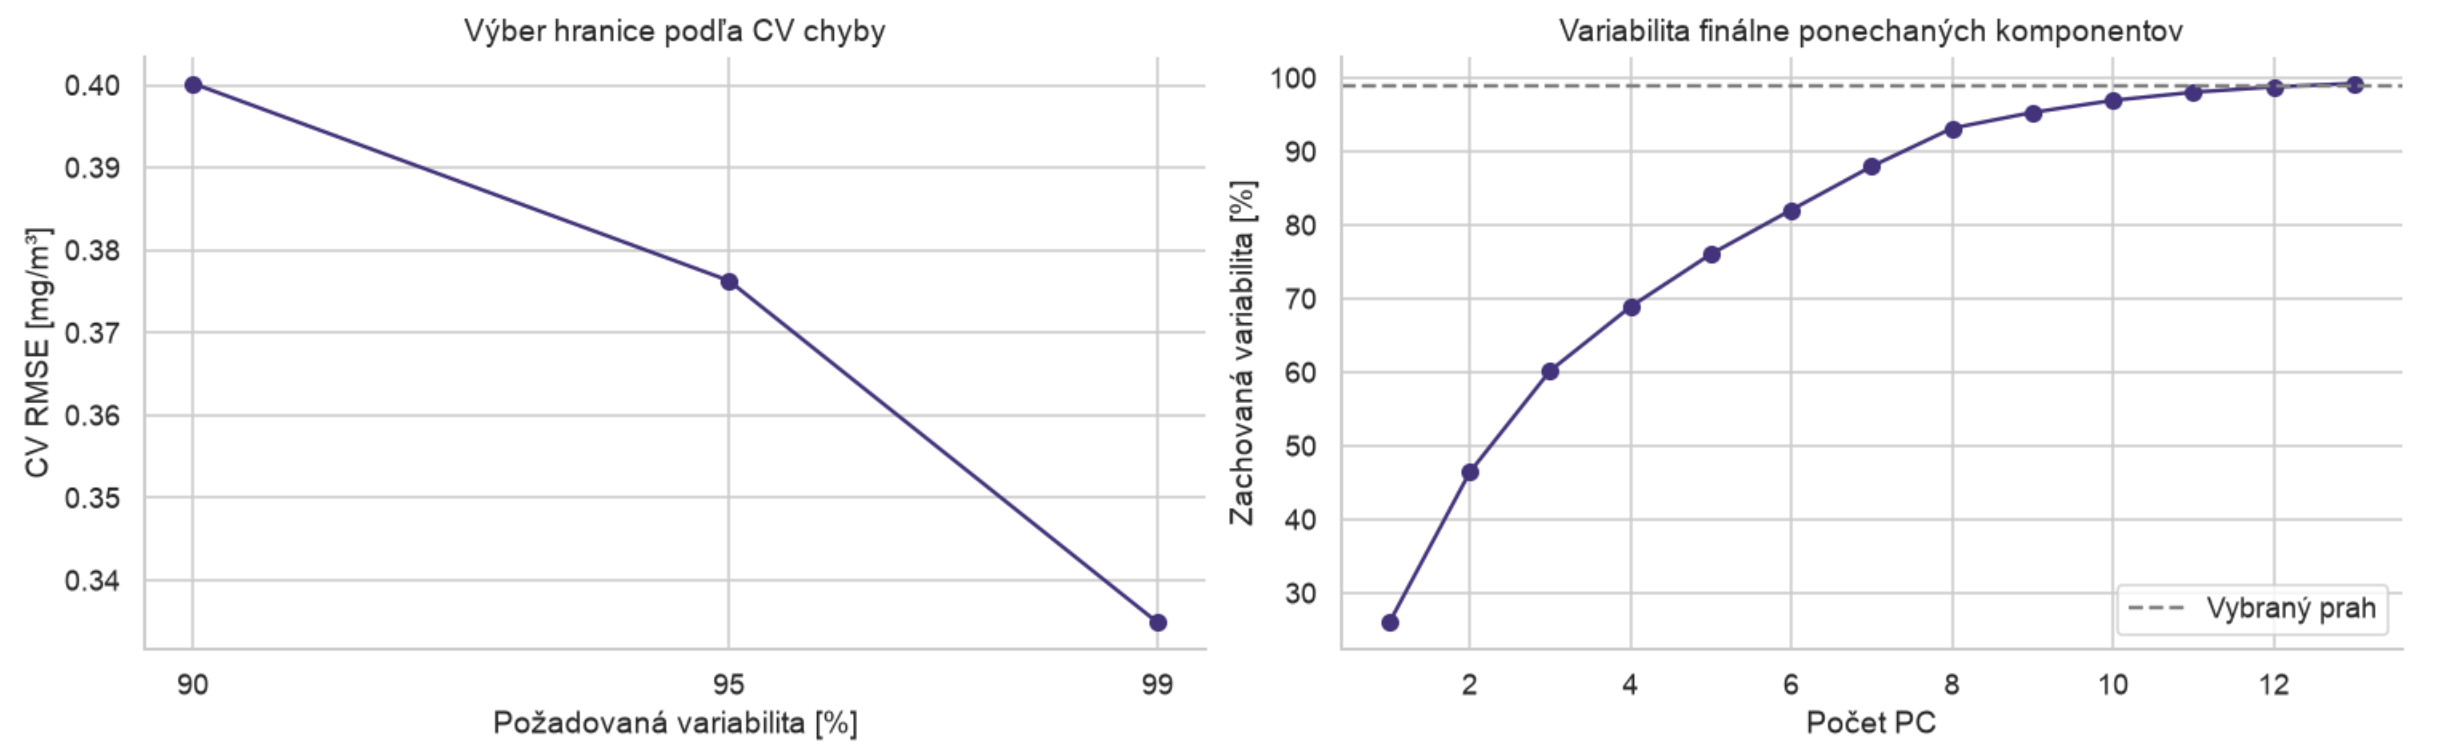
\includegraphics[width=\linewidth,keepaspectratio]{pca_vyber_prahu_variancie_graf.png}
\end{minipage}\hfill%
\begin{minipage}[c]{0.33\linewidth}
\centering
\small\textbf{CV výsledky prahov}\par\smallskip
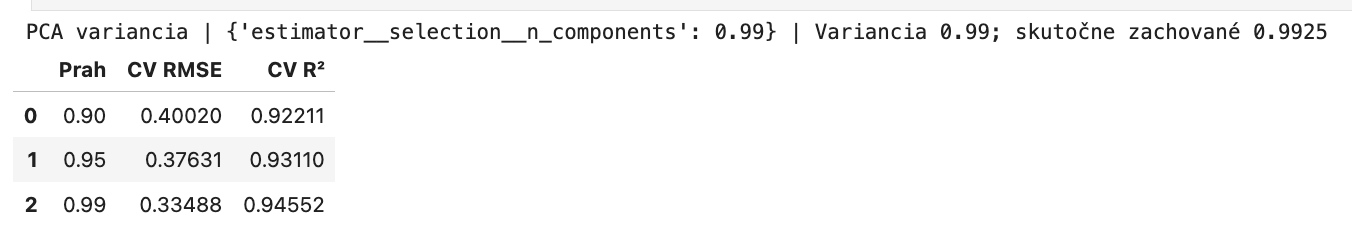
\includegraphics[width=\linewidth,keepaspectratio,trim=4bp 12bp 506bp 28bp,clip]{pca_vyber_prahu_variancie_tabulka.png}
\end{minipage}
\end{center}

% main.ipynb: bunka 130
\textbf{Prah 99\%:} 13 komponentov ponechá \textbf{99.25 \%} a zahodí \textbf{0.75 \%} vstupnej variability. Rekonštrukčná RMSE je 0.0866 v z jednotkách. Percento je skutočne dosiahnutý podiel: pre diskrétny počet komponentov môže presiahnuť zadaný prah.

% main.ipynb: bunka 147
\textbf{PCA variancia:} 13 vstupov, testovacie \(R^2\) \textbf{0.9478}, RMSE \textbf{0.3289 \(\mathrm{mg}/\mathrm{m}^3\)}, rozdiel RMSE oproti plnému modelu +0.0213 \(\mathrm{mg}/\mathrm{m}^3\). Zmenšenie tu neprinieslo nižšiu chybu. Úspora rozmerov môže stáť predikčnú informáciu.

% main.ipynb: bunka 149
\subsection{Porovnanie}

% main.ipynb: bunka 149
Porovnám pôvodný model a všetky tri stratégie na totožných testovacích meraniach. Okrem výsledných chýb sledujem aj počet vstupov a reziduály.

\begin{center}
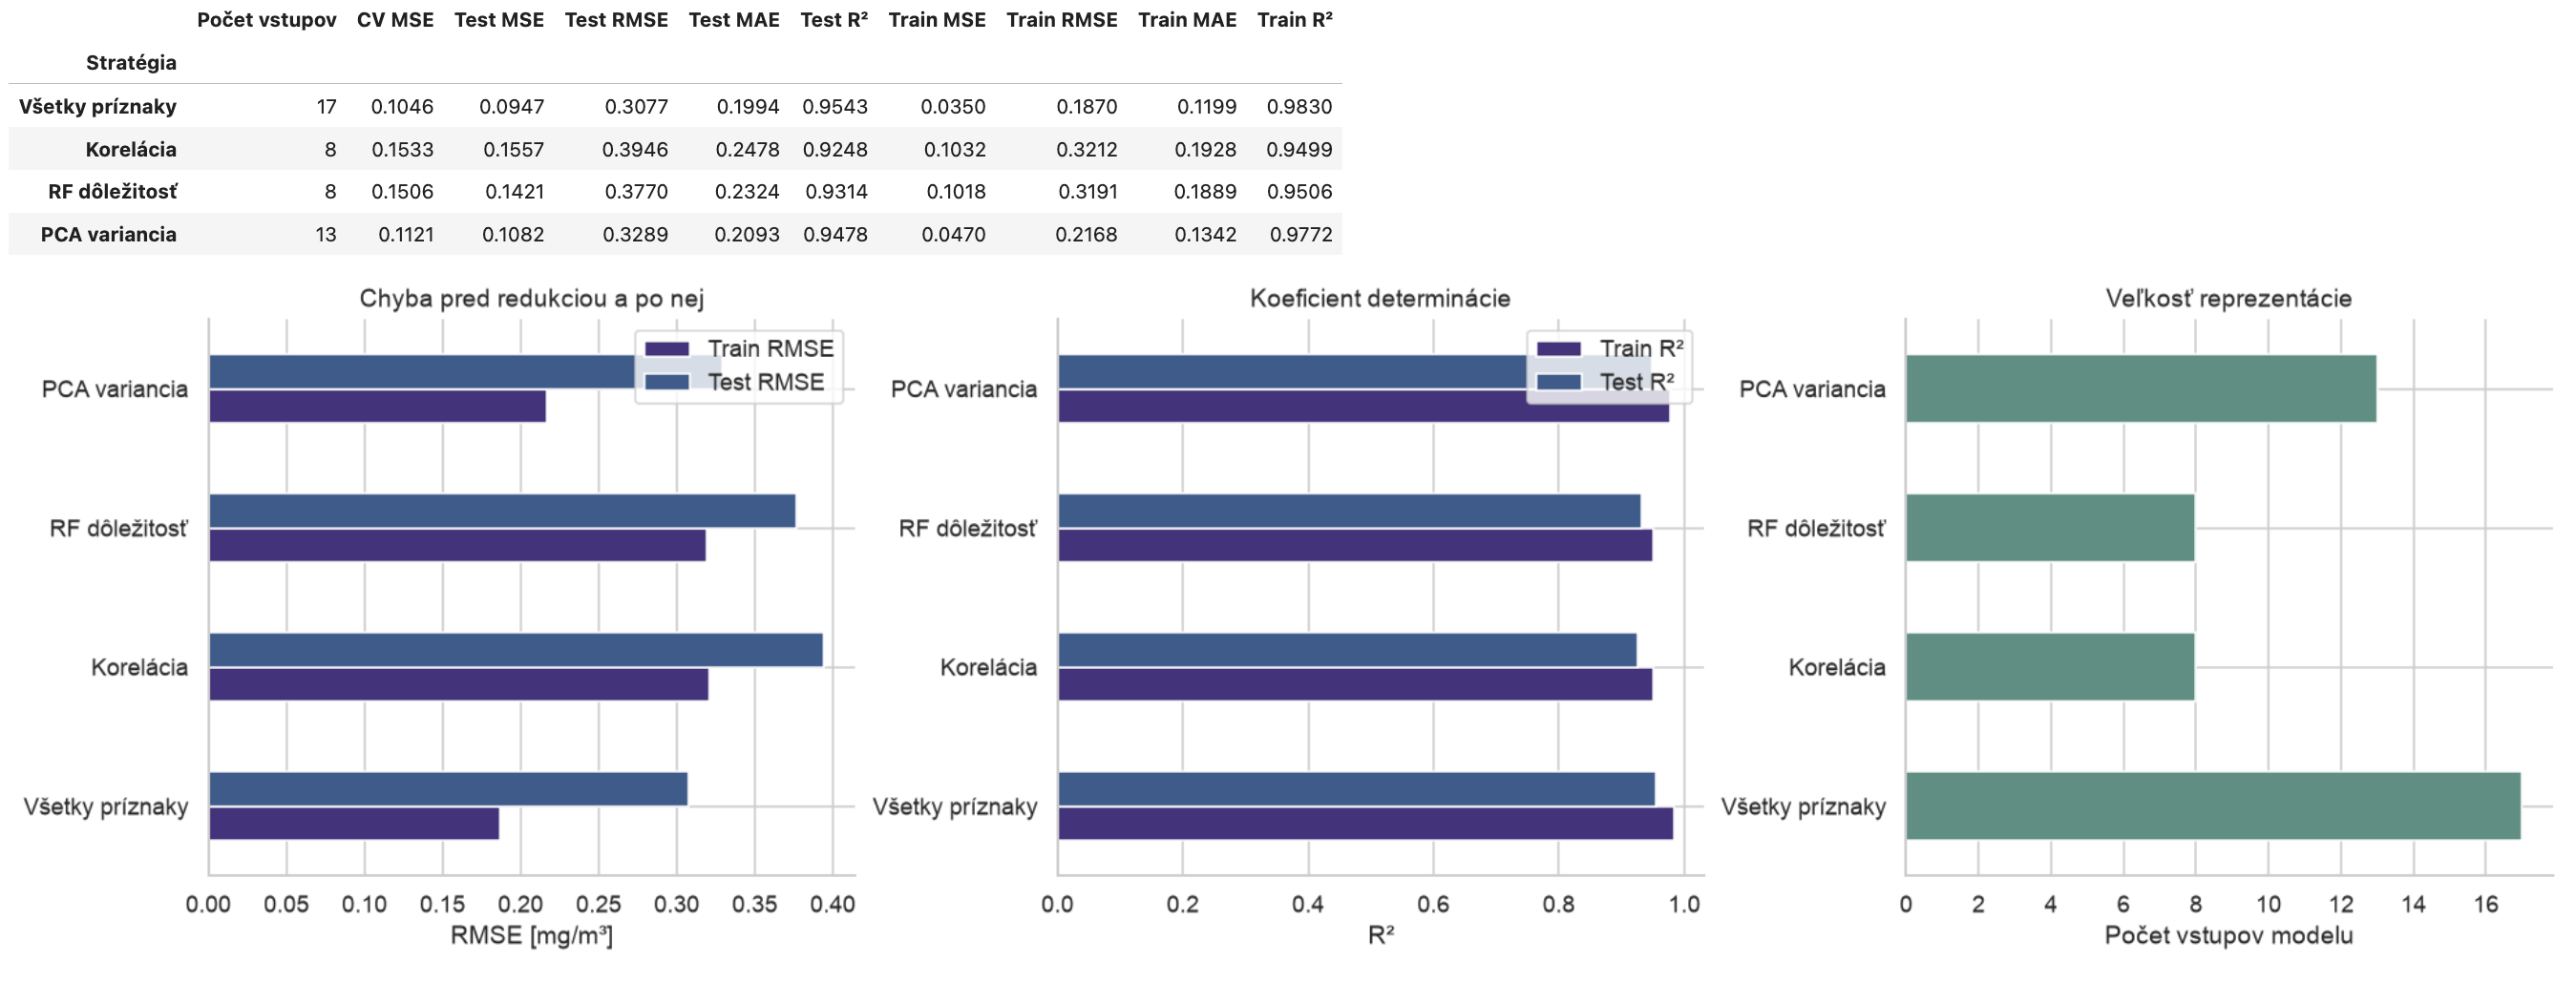
\includegraphics[width=\linewidth,keepaspectratio]{redukcia_porovnanie_strategii.png}
\end{center}

% main.ipynb: bunka 148
V tomto experimente PCA s hranicou 99 \% ponechalo 13 komponentov a skutočne zachovalo približne 99,25 \% vstupnej variability. Aj tak testovacia RMSE SVR vzrástla približne z 0,3077 na 0,3289 \(\mathrm{mg}/\mathrm{m}^3\). Strata len 0,75 \% vstupného rozptylu teda \textbf{neznamená} rovnakú relatívnu zmenu regresnej chyby. PCA nepozná CO a nemôže zaručiť, že zahodí iba nepotrebnú informáciu. Naproti tomu tri komponenty pre obrázok zachovávajú len približne 60,2 \%, preto ich nepovažujem za rovnocennú náhradu zvolenej 13D regresnej reprezentácie.

% main.ipynb: bunka 152
\subsubsection{Reziduály po redukcii}

% main.ipynb: bunka 152
Rovnaké testovacie riadky a spoločné osi umožňujú porovnať, či redukcia zväčšuje rozptyl alebo podhodnotenie pri vysokom CO. Korelačný výber zachytáva lineárny vzťah s cieľom, ensemble aj nelinearity, PCA predovšetkým veľké smery variability. Preto ich poradie podľa zachovanej variability nemusí súhlasiť s poradím predikčnej chyby.

\begin{center}
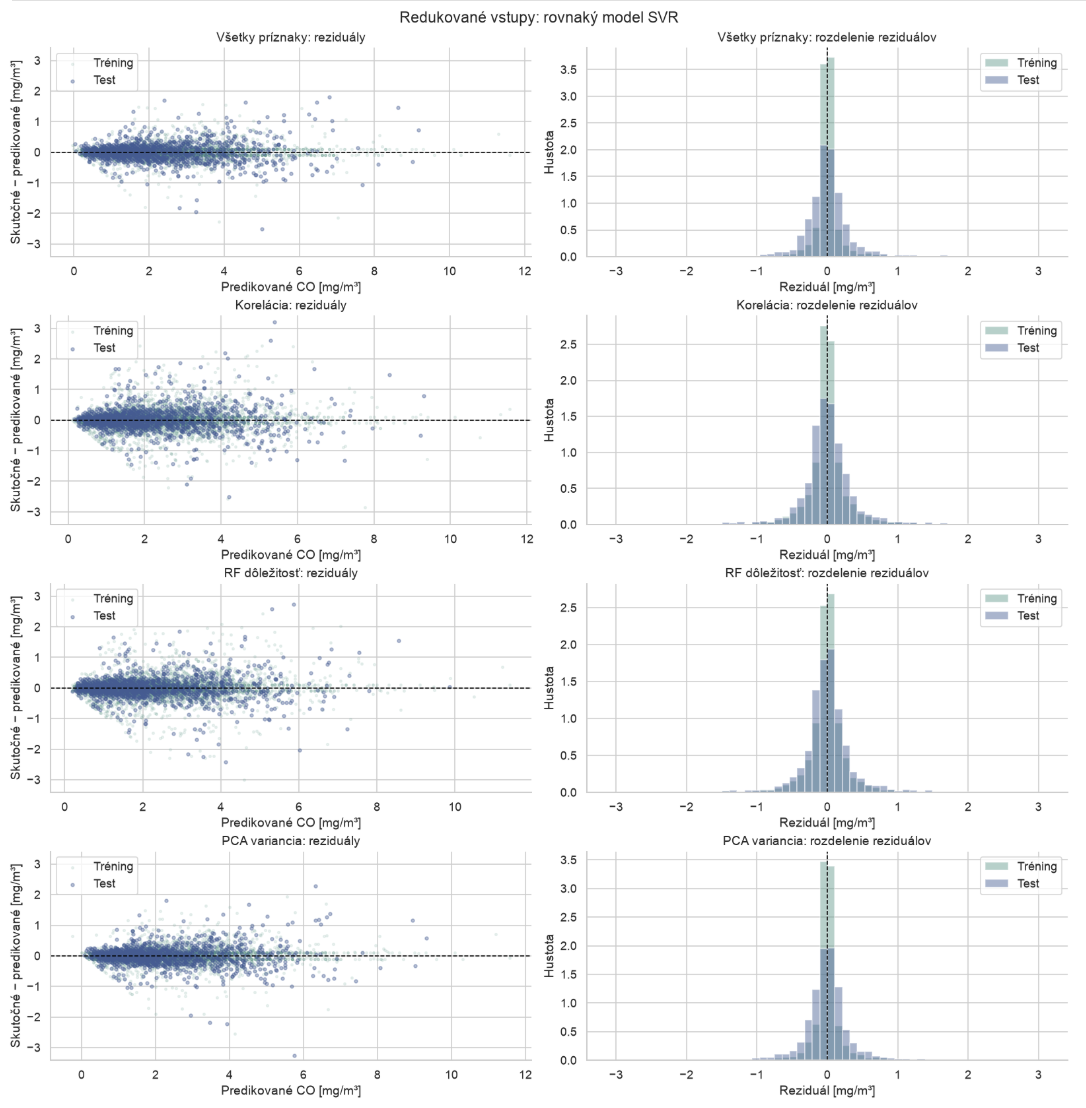
\includegraphics[width=0.91\linewidth,keepaspectratio,height=0.66\textheight]{redukcia_rezidualy_graf.png}
\end{center}

\begin{center}
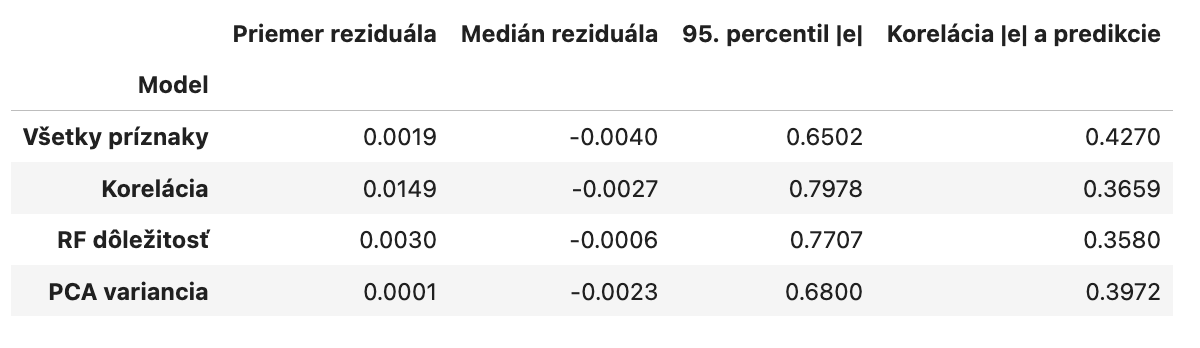
\includegraphics[width=\linewidth,keepaspectratio,height=0.17\textheight]{redukcia_rezidualy_tabulka.png}
\end{center}


% main.ipynb: bunka 155
\section{Zhlukovanie -- bonus}

% main.ipynb: bunka 155
\subsection{Vizualizácia}

% main.ipynb: bunka 155
K-means sa učí na \textbf{všetkých 17 štandardizovaných vstupoch}, bez CO a iba z tréningových inlierov. Porovnávam 3, 4 a 5 zhlukov pomocou silhouette skóre na rovnakej tréningovej podvzorke. Vyberám najvyššie skóre, nie najlepšiu regresiu na teste.

% main.ipynb: bunka 157
Vybral som \textbf{4 zhluky} so silhouette \textbf{0.252}. Hodnota blízko nule znamená slabé oddelenie, hodnota blízko jednej kompaktné a oddelené skupiny. Vedľa porovnania silhouette skóre je lakťová metóda: inertia je súčet štvorcov vzdialeností k centroidom v 17D. Lakeť hľadám tam, kde ďalšie zhluky prinášajú už len malý pokles. Prerušovaná čiara označuje \(k=4\), vybrané podľa silhouette spomedzi 3, 4 a 5.

\begin{center}
\begin{minipage}[c]{0.49\linewidth}
\centering
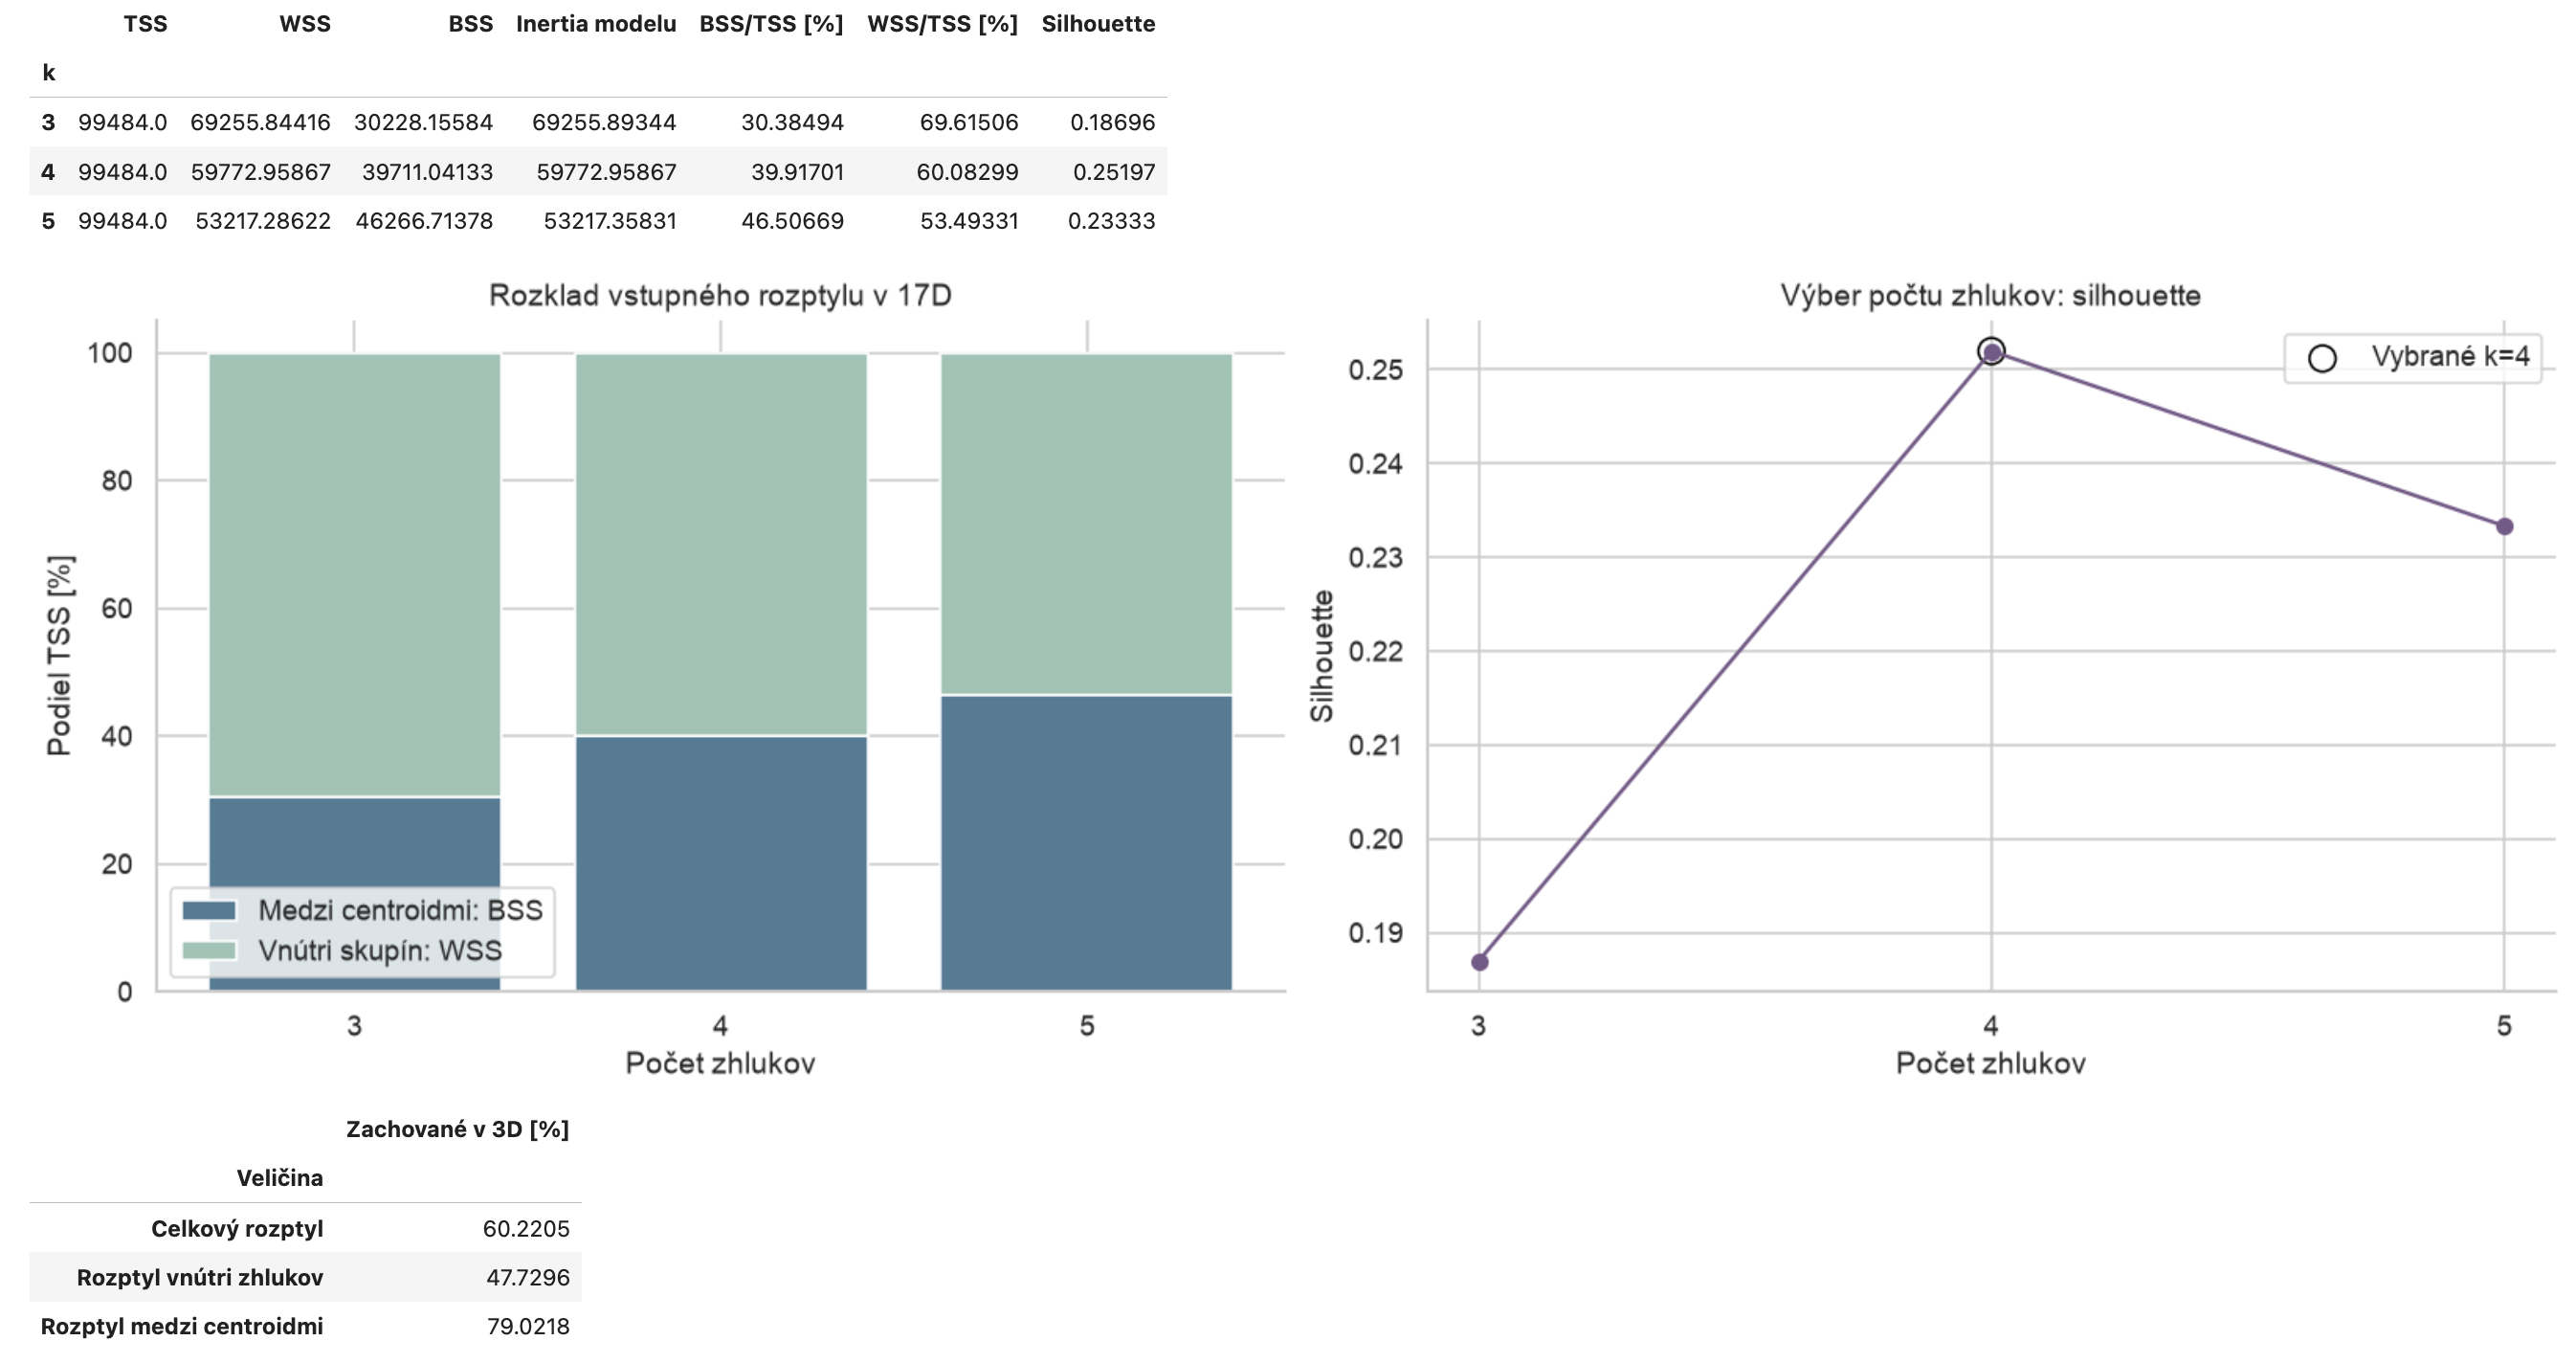
\includegraphics[width=\linewidth,keepaspectratio]{kmeans_vyber_poctu_zhlukov.png}
\end{minipage}\hfill%
\begin{minipage}[c]{0.49\linewidth}
\centering
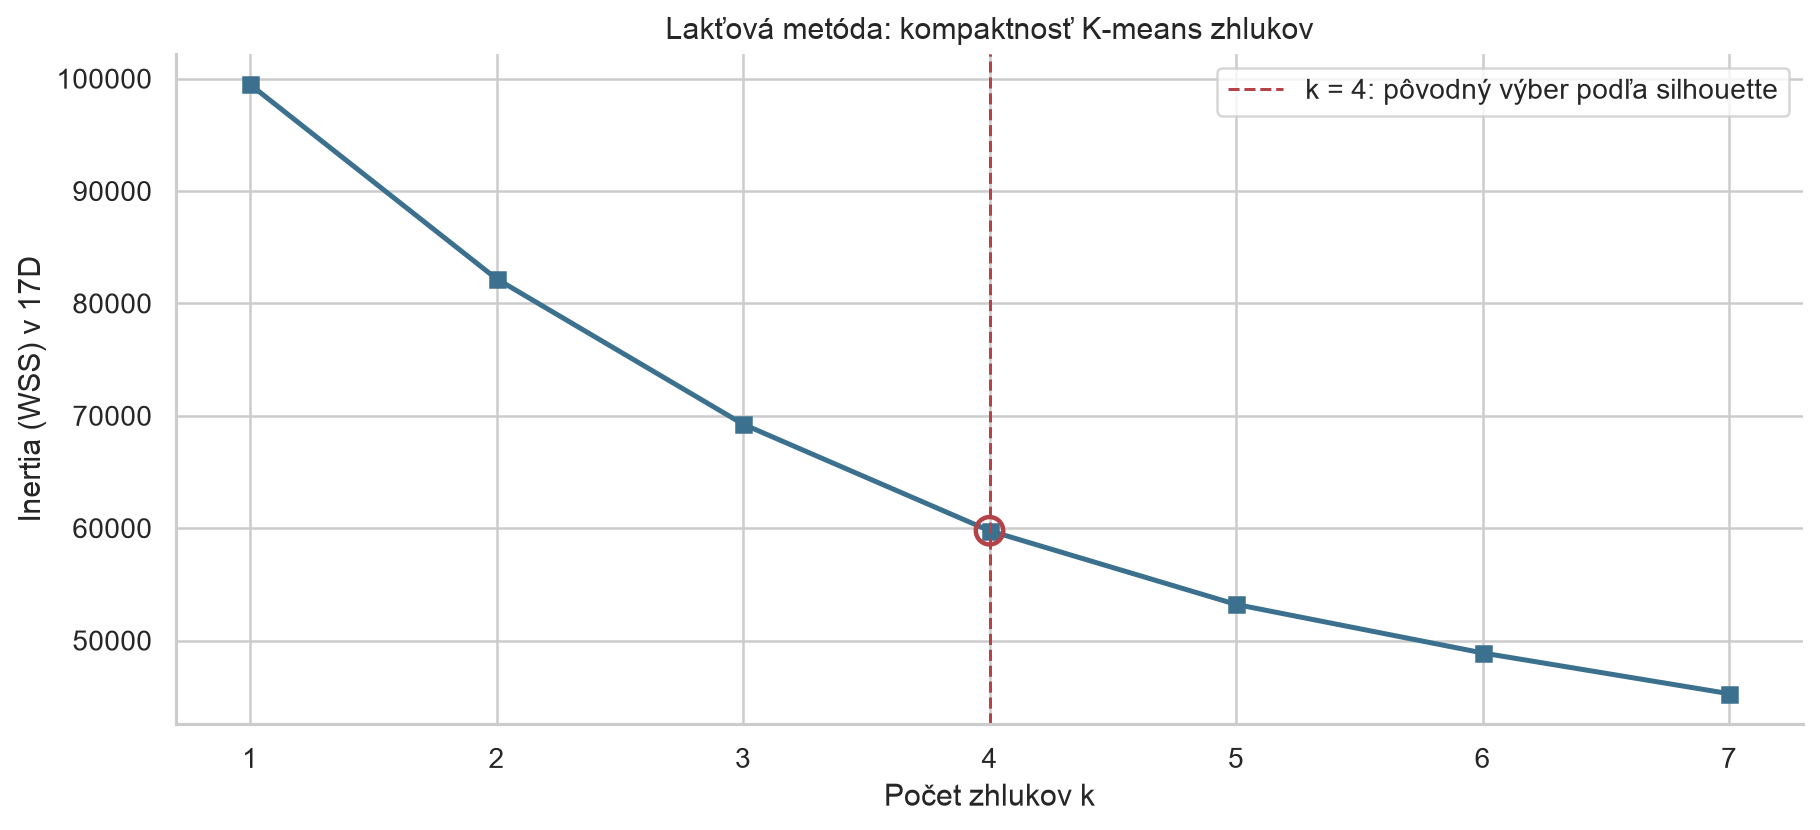
\includegraphics[width=\linewidth,keepaspectratio]{kmeans_laktova_metoda_graf.png}
\end{minipage}
\end{center}

Grafy nižšie zobrazujú tie isté štyri zhluky z viacerých pohľadov a prvé kroky algoritmu K-means. Farba bodu označuje zhluk, čísla zhlukov sú ľubovoľné označenia. V 3D grafe sú osi tri PCA súradnice, preto prekryv v projekcii nemusí znamenať prekryv v plnom priestore.

\begin{center}
\begin{minipage}[c]{0.49\linewidth}
\centering
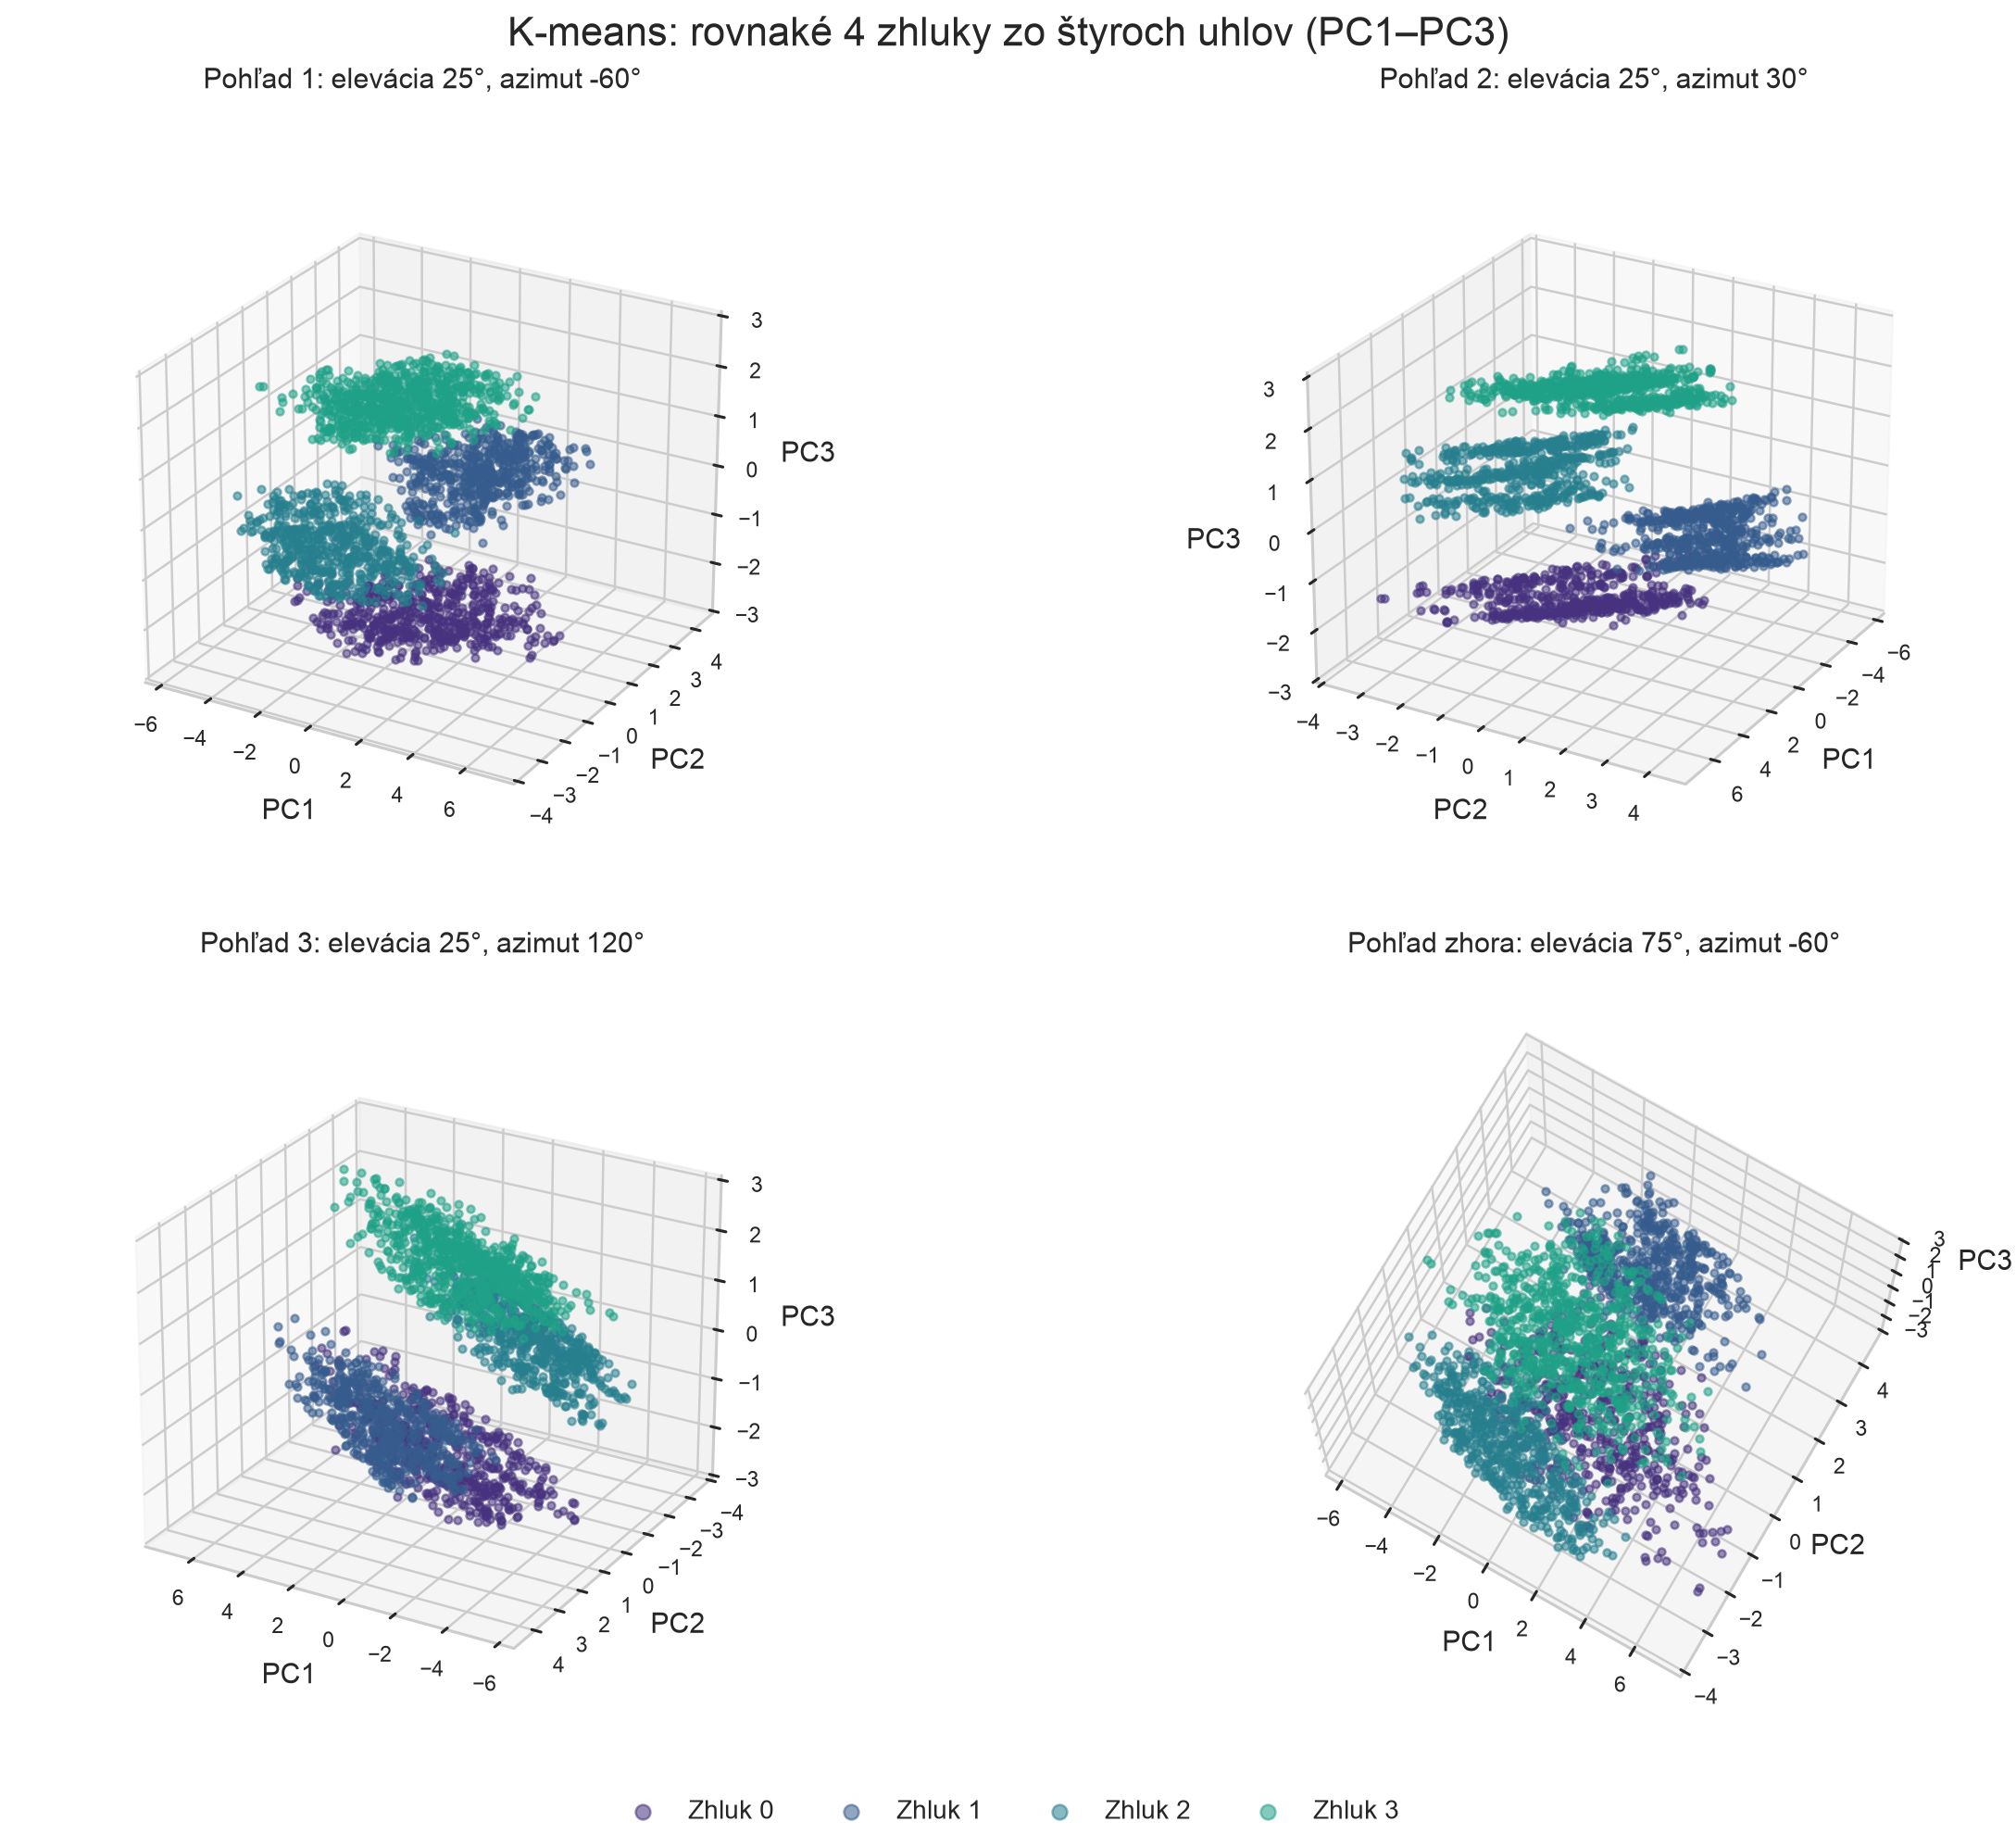
\includegraphics[width=\linewidth,keepaspectratio]{kmeans_zhluky_viac_pohladov_graf.png}
\end{minipage}\hfill%
\begin{minipage}[c]{0.49\linewidth}
\centering
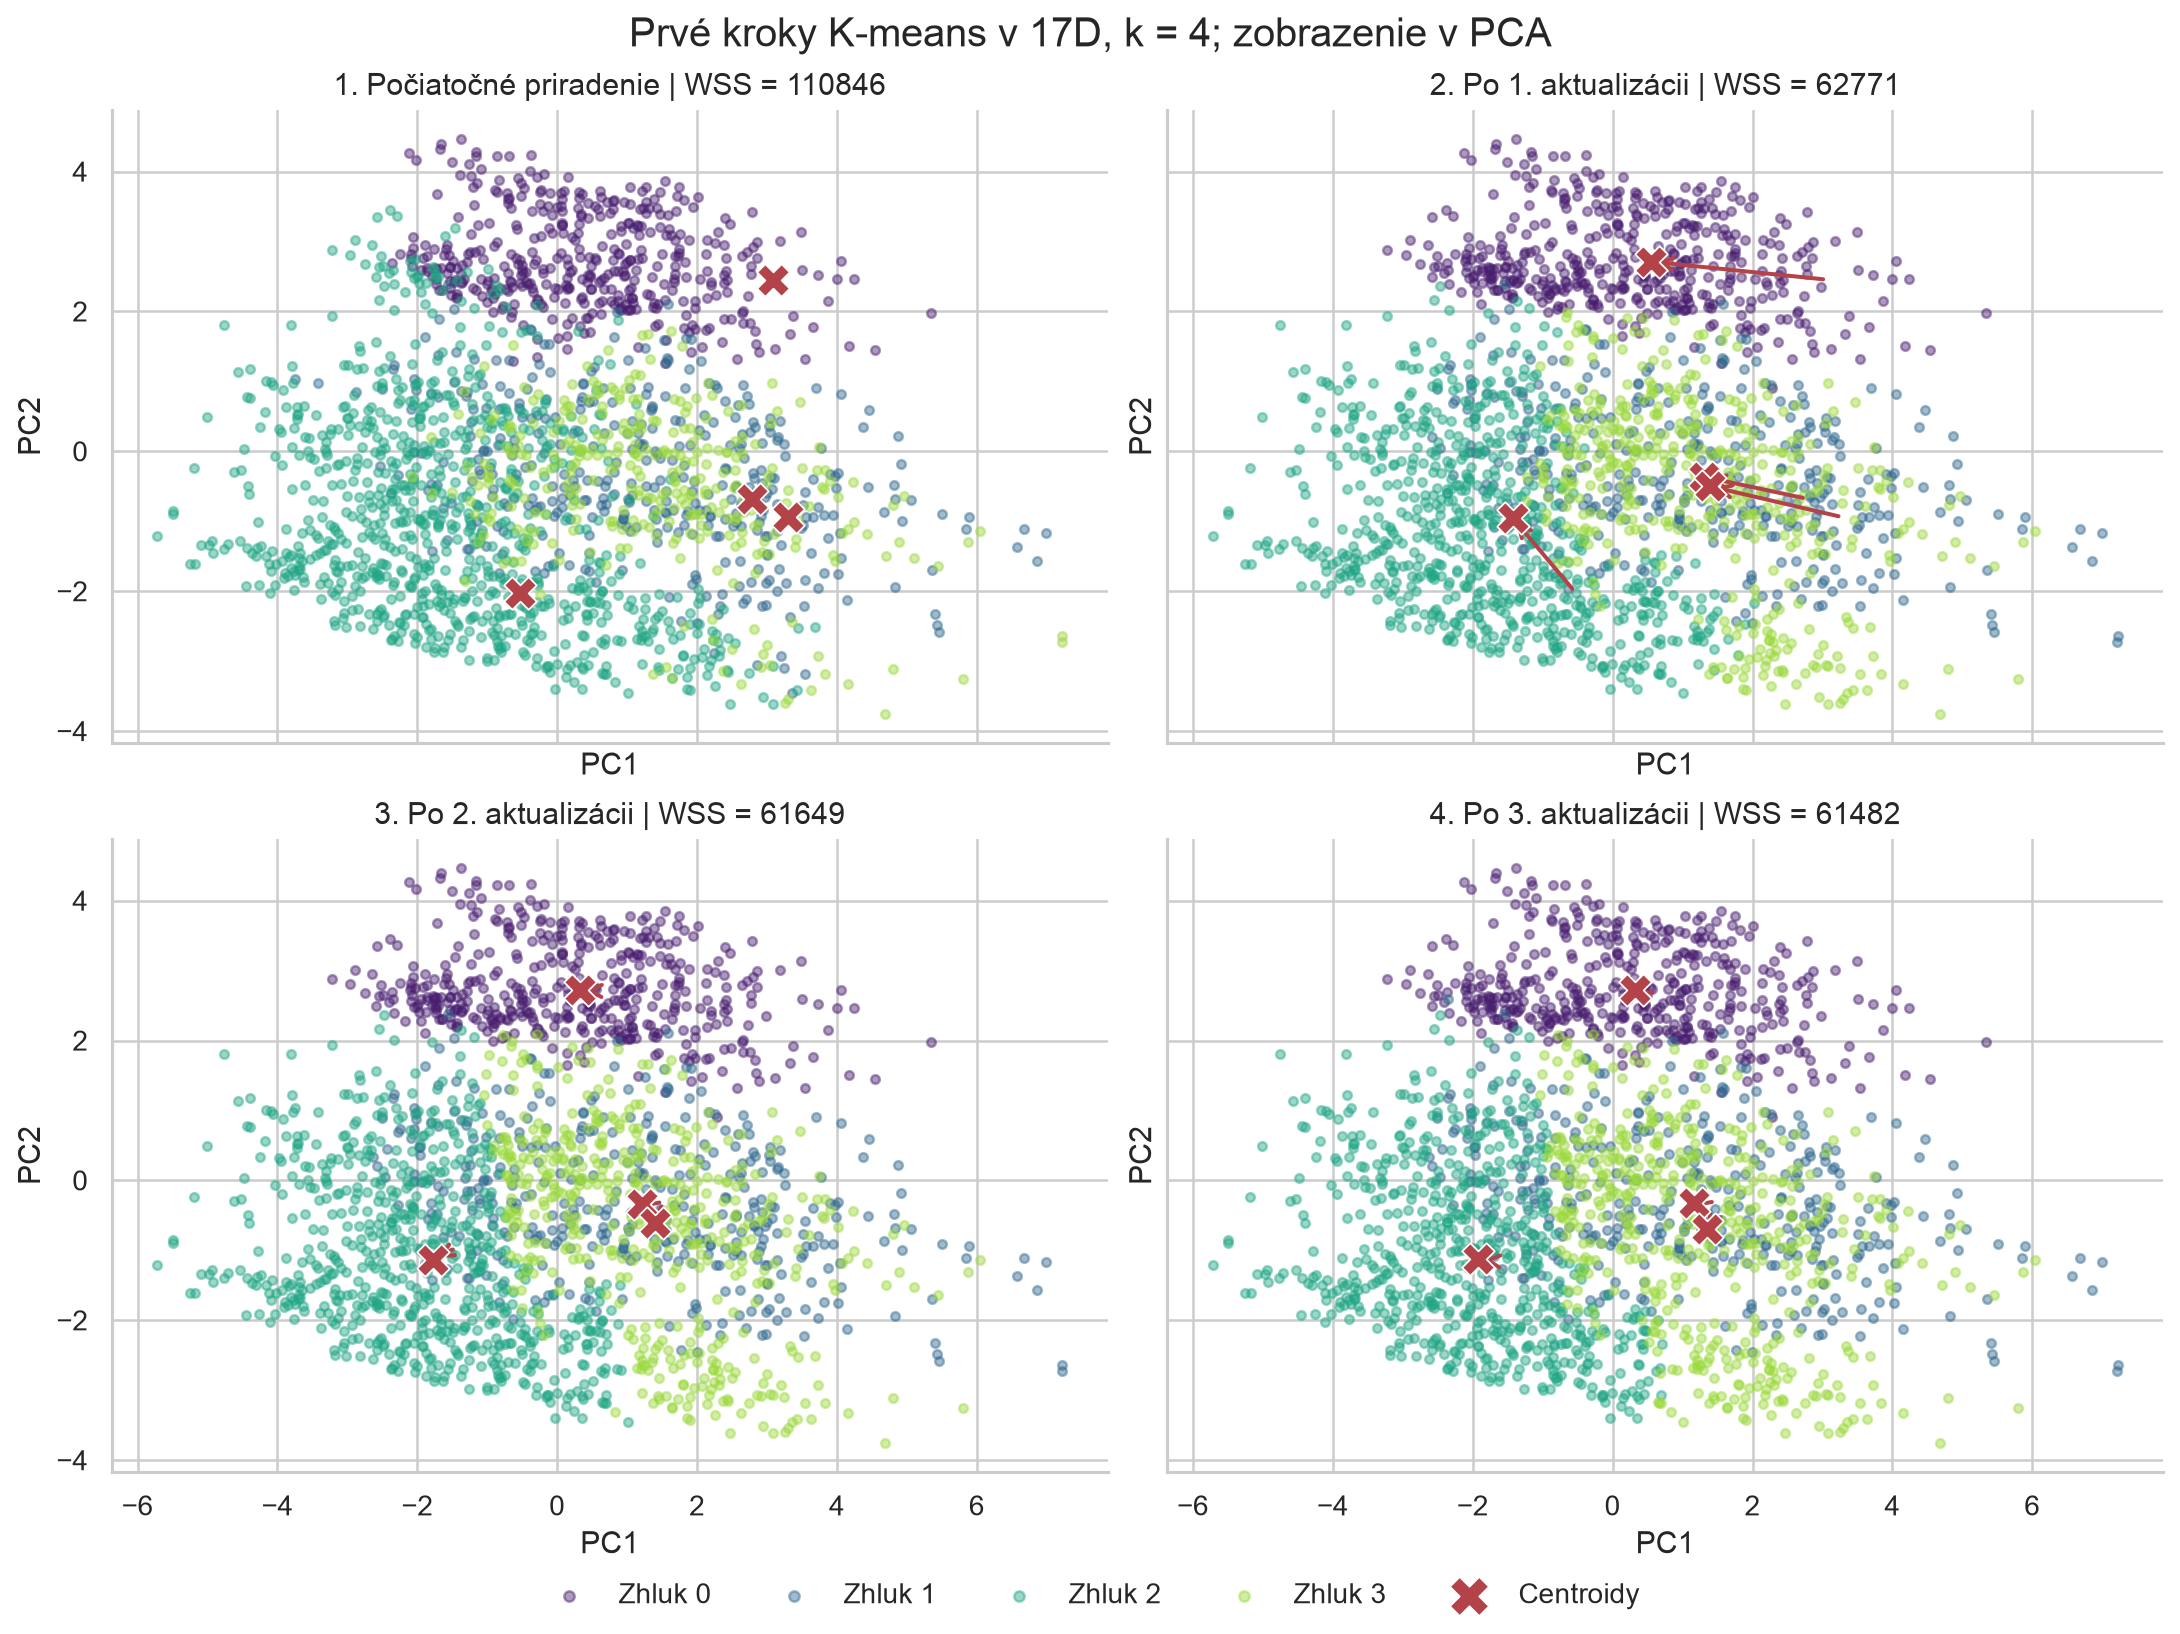
\includegraphics[width=\linewidth,keepaspectratio]{kmeans_priebeh_iteracii_graf.png}
\end{minipage}
\end{center}

Výpočty a WSS používajú všetky tréningové inliery v 17D. V priebehu iterácií sú zobrazené iba PC1 a PC2 a rovnaká podvzorka najviac 2\,000 bodov. Priradenie farby preto nemusí zodpovedať najbližšiemu centroidu v tejto 2D projekcii. Profily v nasledujúcej časti ukazujú mediány pôvodných senzorov a počasia.

\subsubsection{Profily zhlukov a strata rozptylu v projekcii}

\begin{center}
\noindent
\begin{minipage}[c]{0.46\linewidth}
\centering
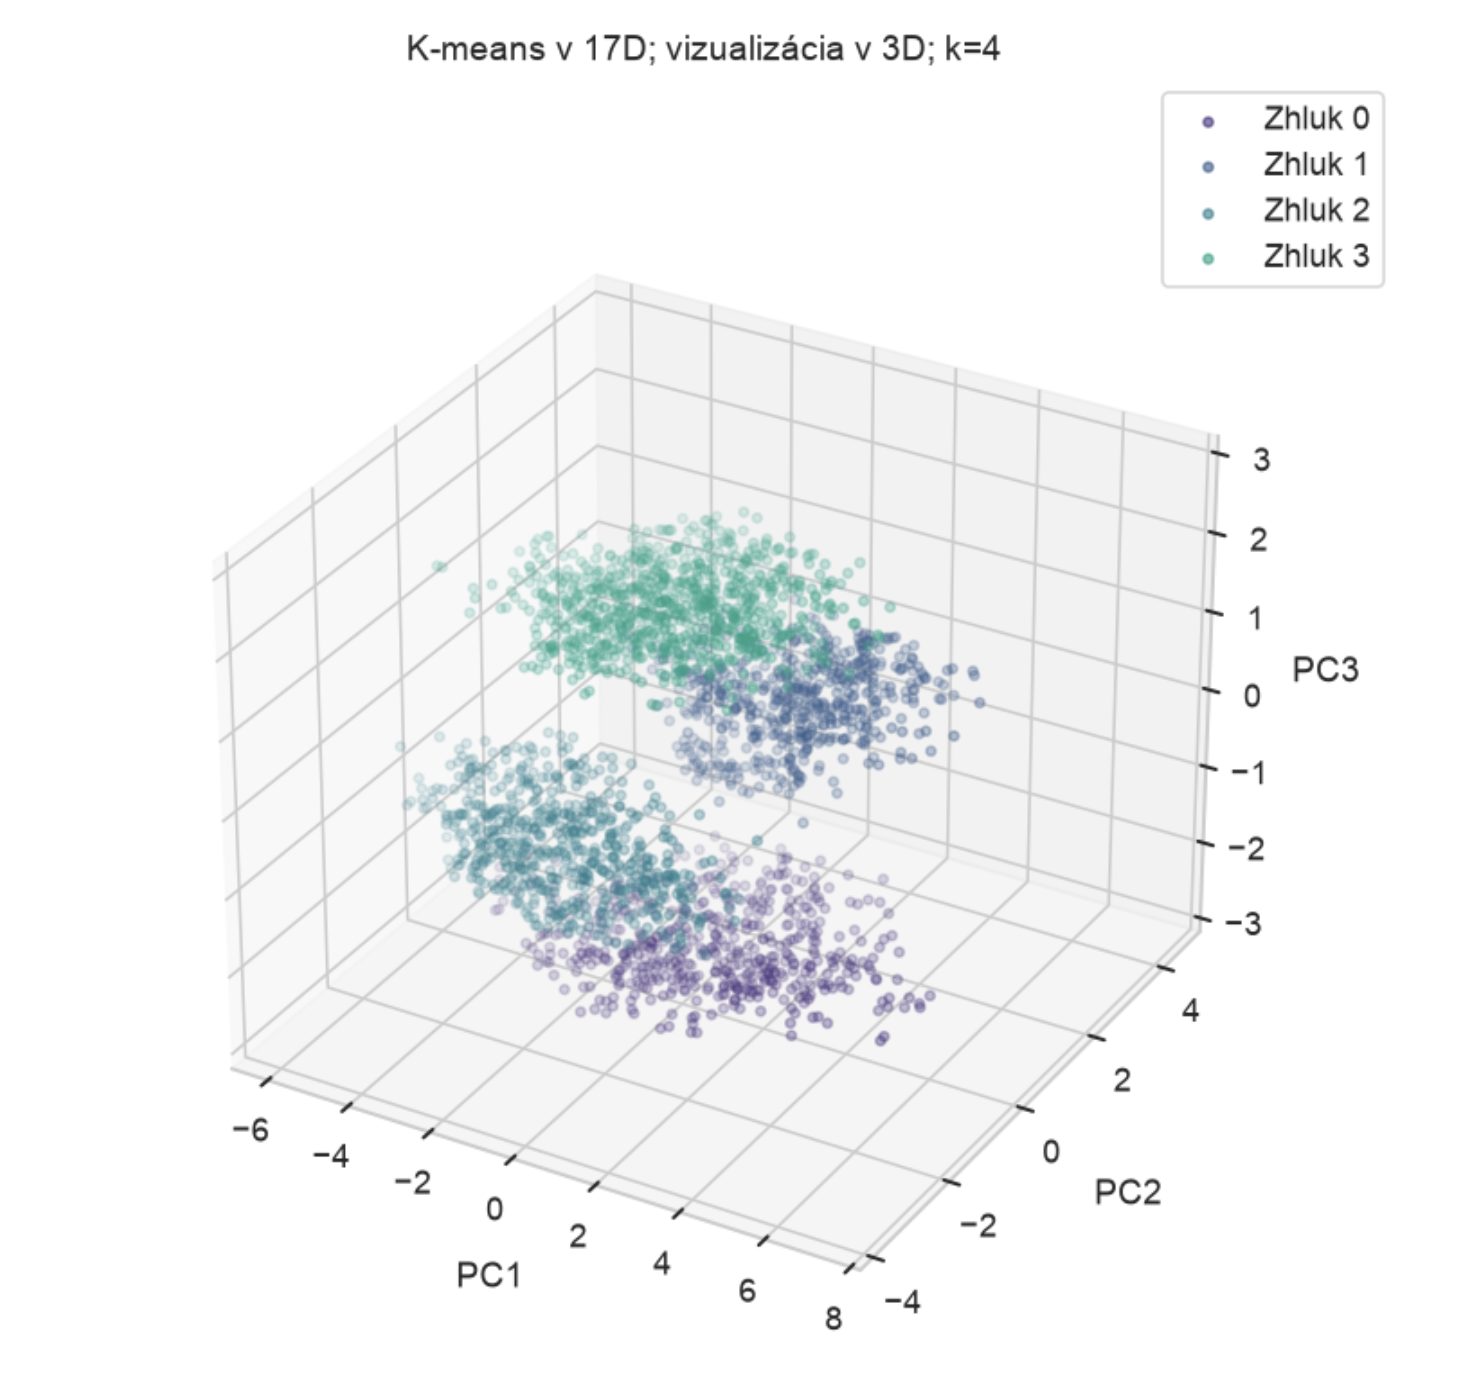
\includegraphics[width=0.8\linewidth,keepaspectratio]{kmeans_zhluky_3d_graf.png}
\end{minipage}\hfill%
\begin{minipage}[c]{0.51\linewidth}
\centering
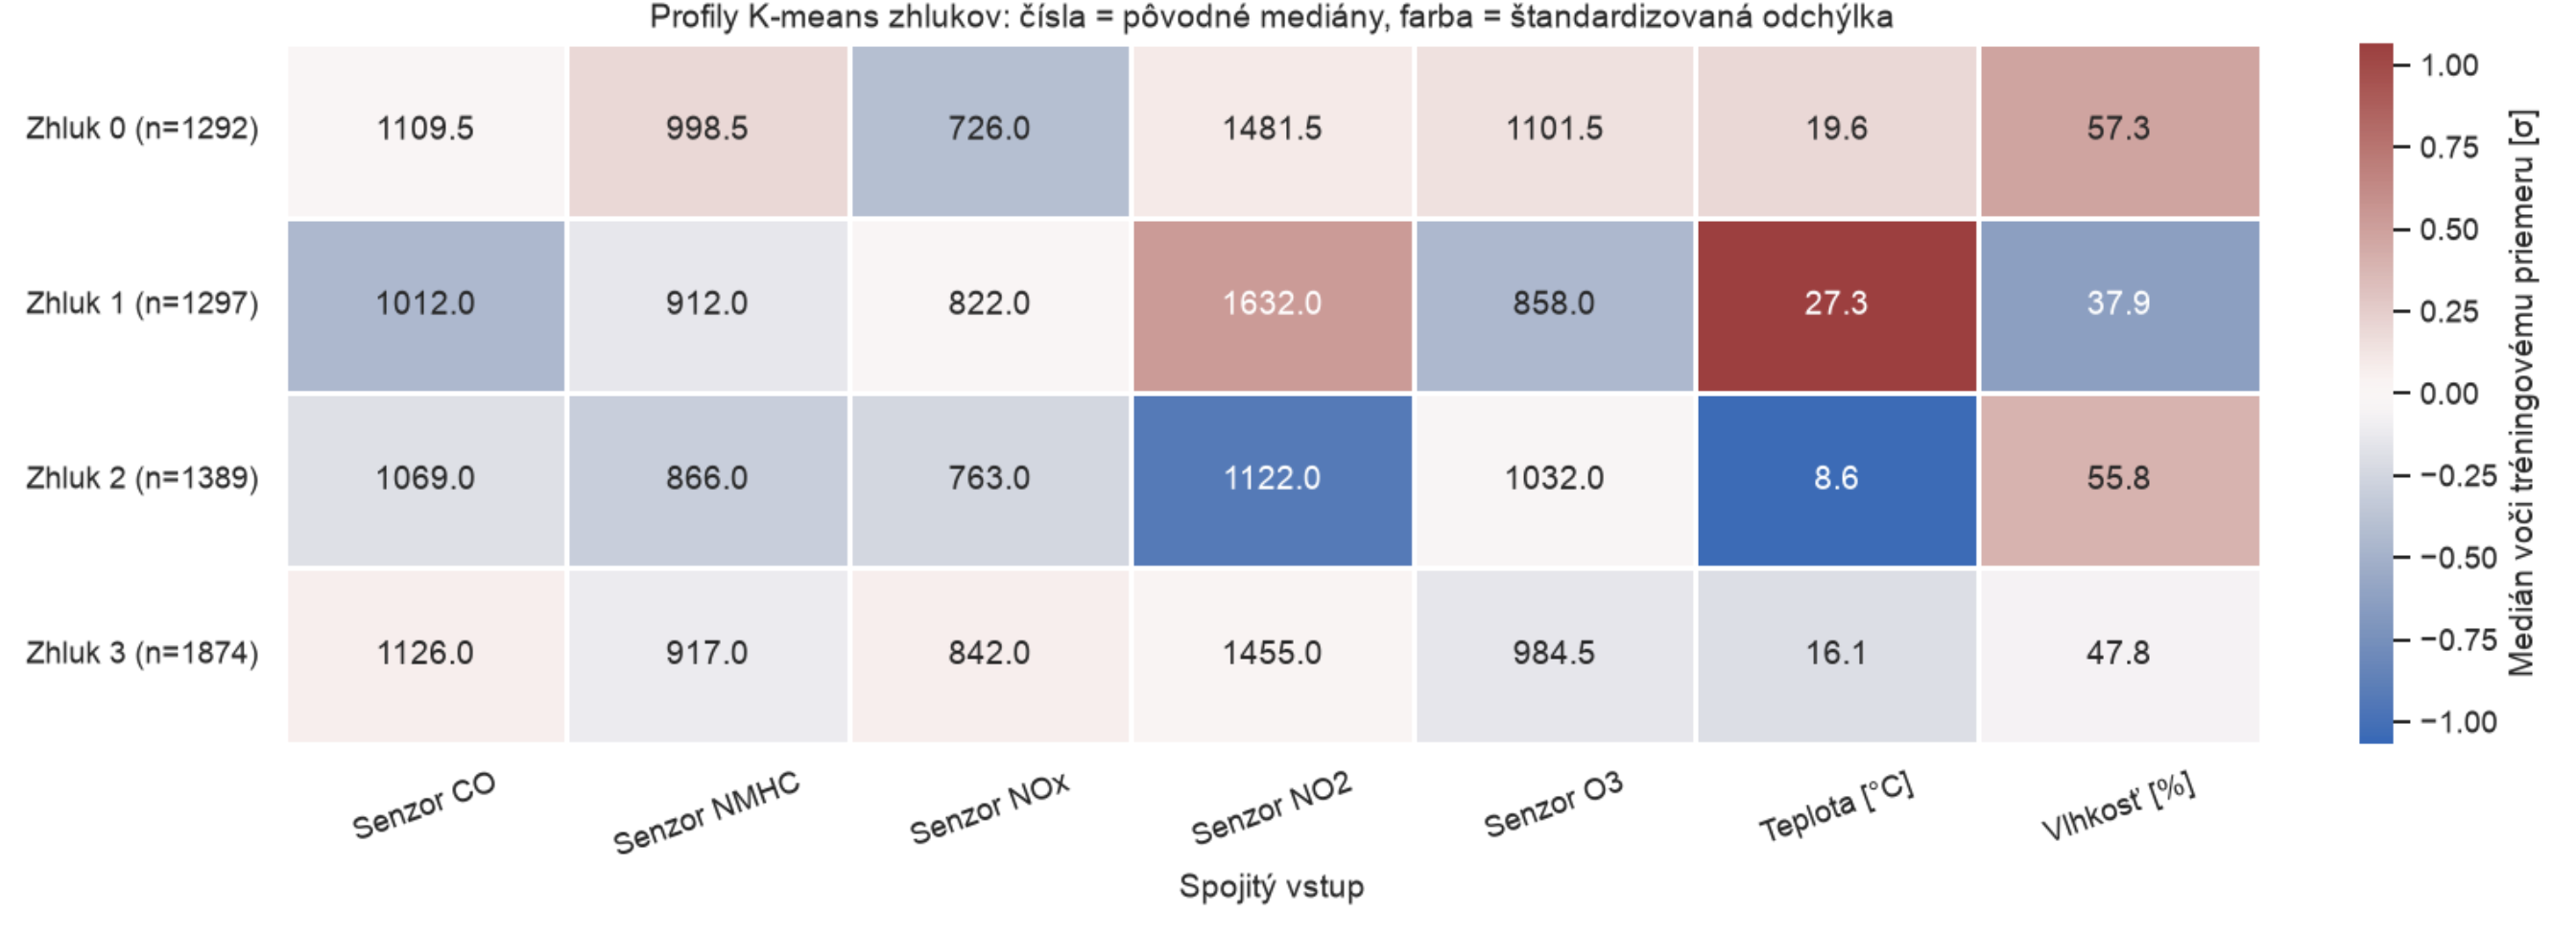
\includegraphics[width=\linewidth,keepaspectratio]{kmeans_profily_zhlukov_graf.png}
\medskip
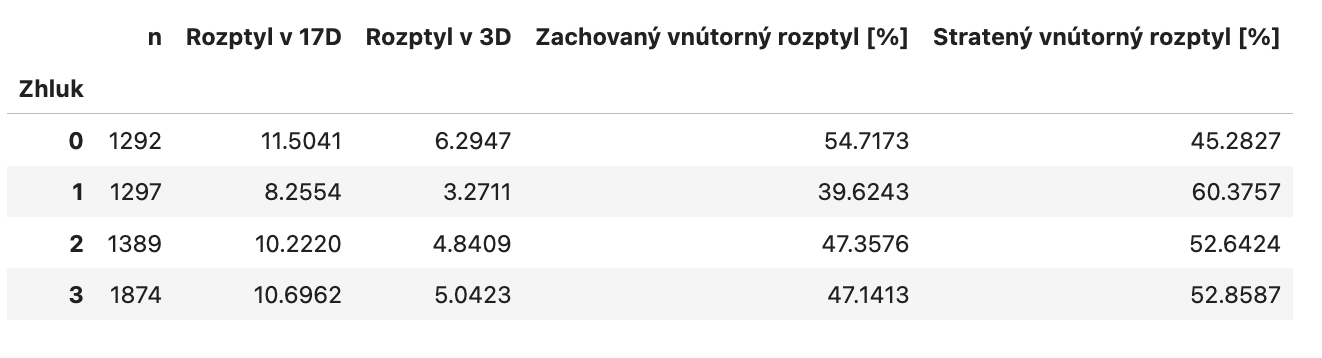
\includegraphics[width=\linewidth,keepaspectratio]{kmeans_rozptyl_zhlukov_v_3d_tabulka.png}
\end{minipage}
\end{center}

Tabuľka profilov uvádza mediány v pôvodných jednotkách. Druhá tabuľka porovnáva vnútorný rozptyl každého zhluku v 17D a jeho zachovanú časť v troch PCA súradniciach. Projekcia preto nezobrazuje celú vnútornú štruktúru zhlukov.



\subsection{Trénovanie}

% main.ipynb: bunka 177
\subsubsection{Globálny model oproti lokálnym expertom}

% main.ipynb: bunka 177
Pre každý zhluk natrénujem model \textbf{rovnakého typu a s rovnakými hyperparametrami} ako CV víťaz prvej časti. Predspracovanie a pravidlo outlierov sa znovu učia len z tréningových bodov daného zhluku. Testovací bod priradí do zhluku tréningový škálovač a K-means. Potom dostane predikciu príslušného lokálneho modelu. Na porovnanie vypočítam aj chybu pôvodného globálneho modelu na presne tých istých bodoch každého zhluku. \(R^2\) v podskupine môže klesnúť aj pre menší rozsah CO. Rozhodujúce je tiež spoločné MSE všetkých bodov.

\begin{center}
\noindent
\begin{minipage}[c]{0.34\linewidth}
\centering
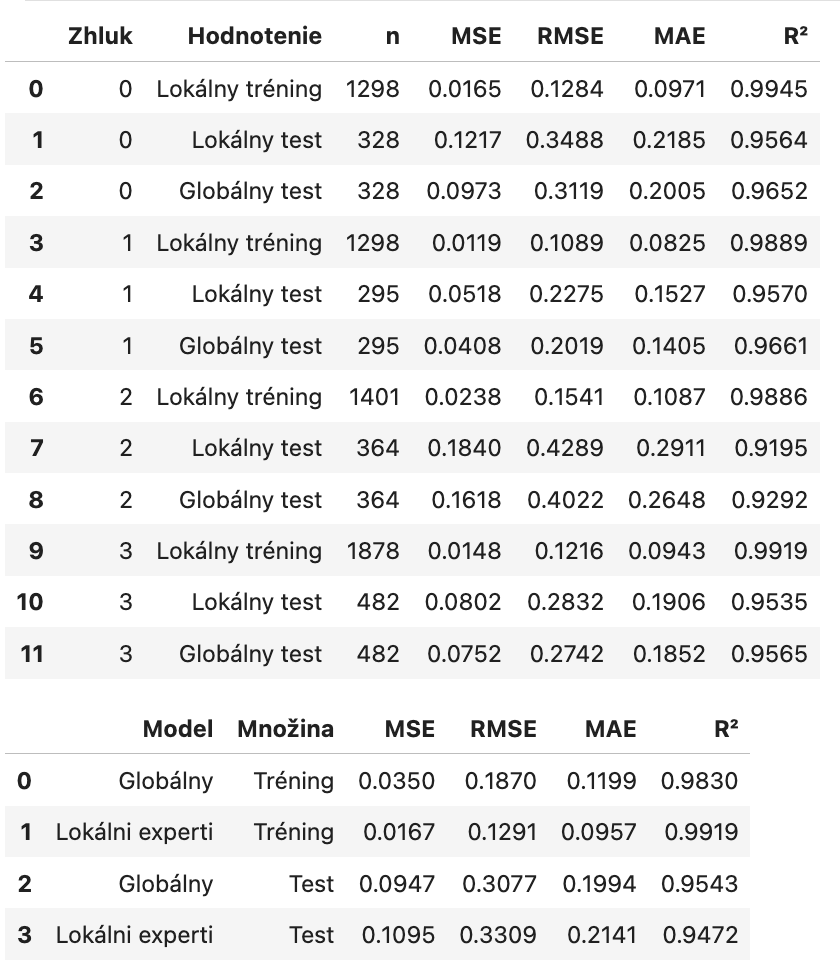
\includegraphics[width=\linewidth,keepaspectratio]{lokalne_modely_porovnanie_metrik_tabulka.png}
\end{minipage}\hfill%
\begin{minipage}[c]{0.63\linewidth}
\centering
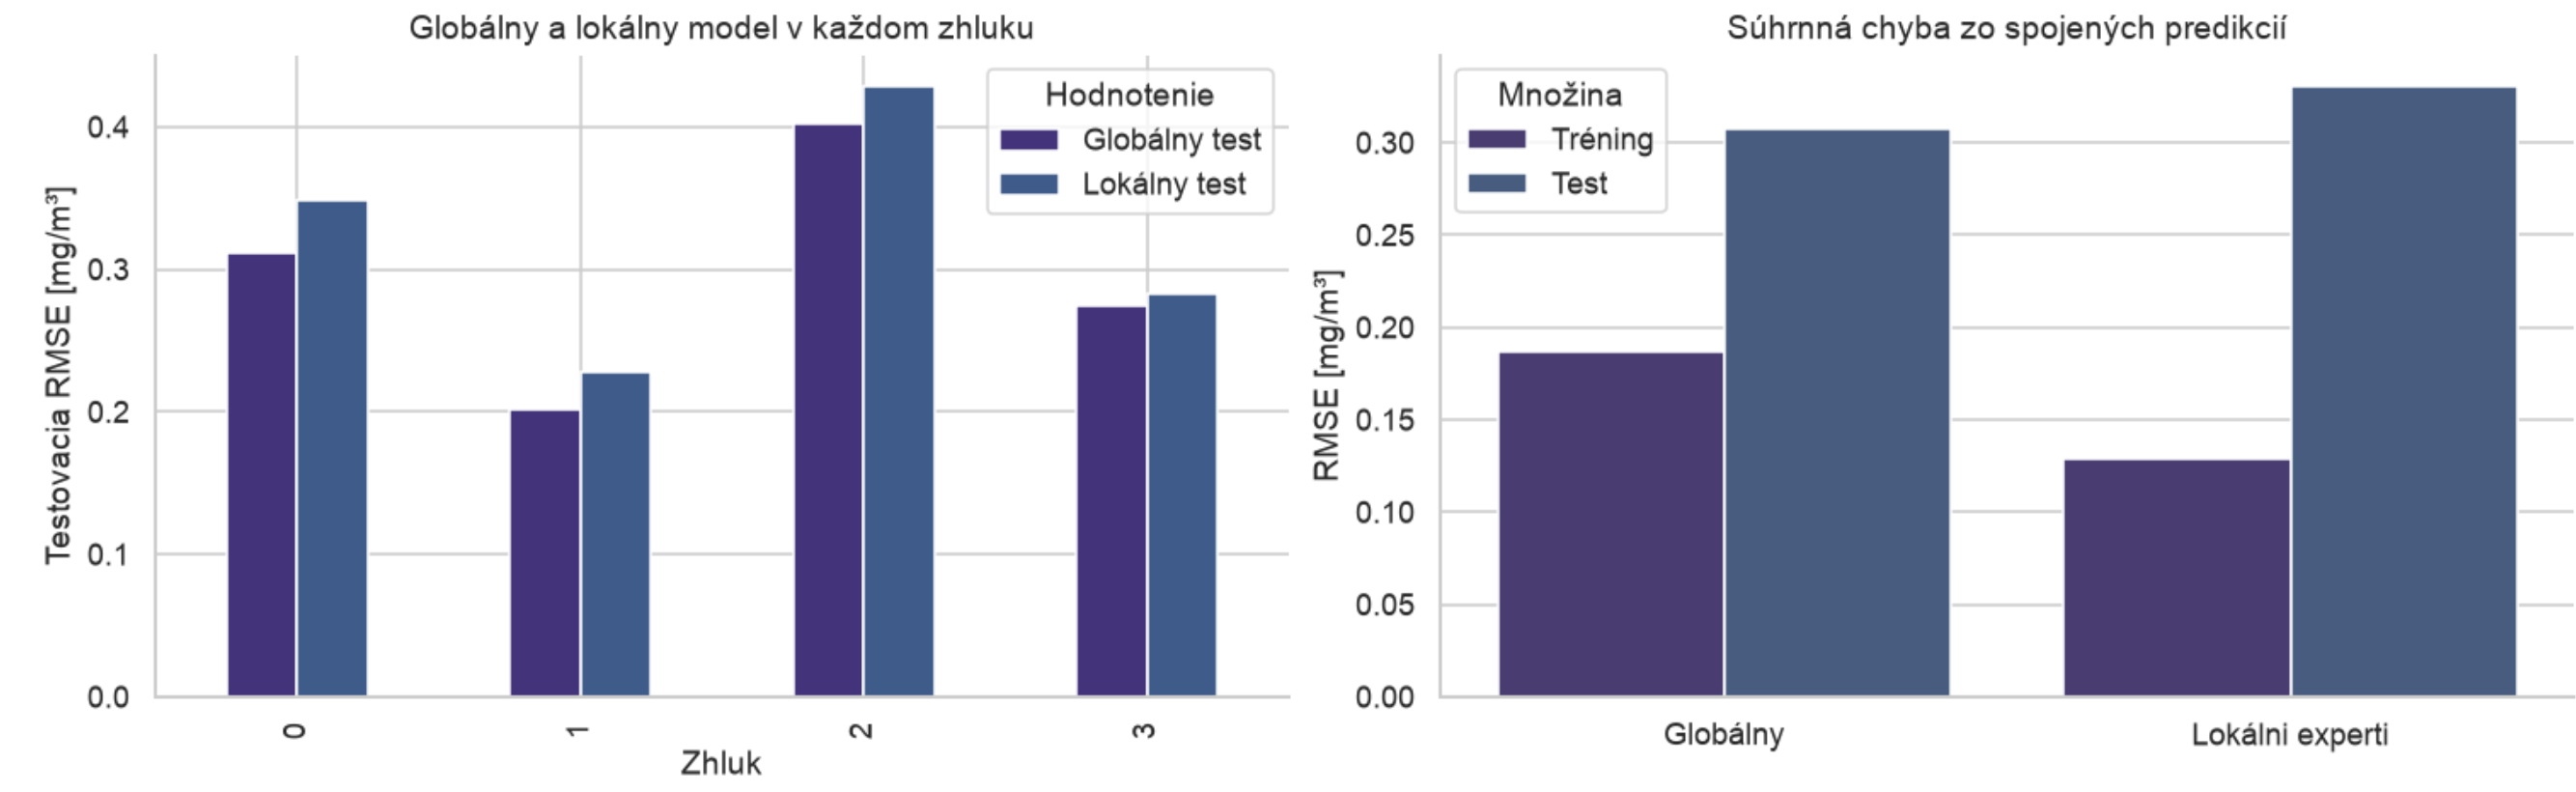
\includegraphics[width=\linewidth,keepaspectratio]{lokalne_modely_porovnanie_rmse_graf.png}
\medskip
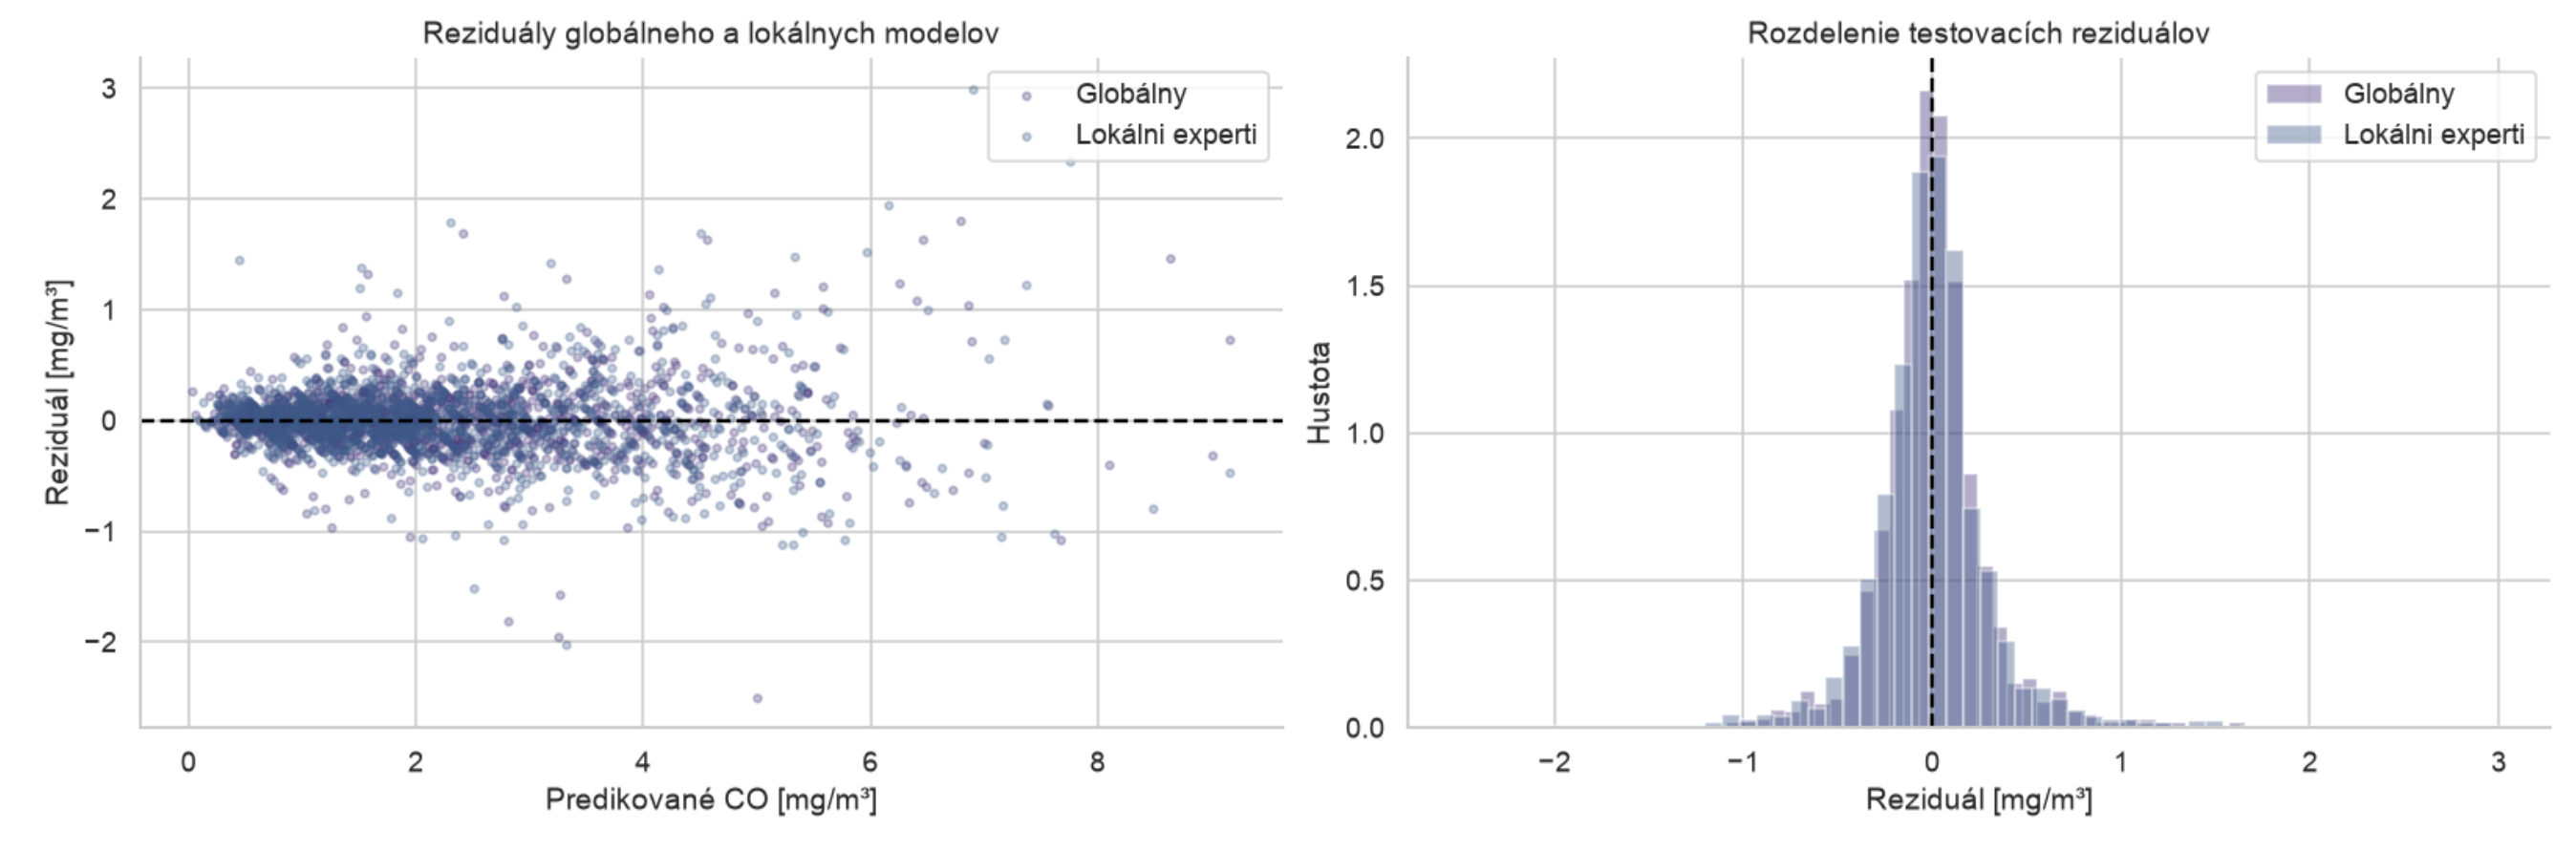
\includegraphics[width=\linewidth,keepaspectratio]{lokalne_modely_rezidualy_graf.png}
\end{minipage}
\end{center}

% main.ipynb: bunka 179
Všetci lokálni experti spolu dosahujú \textbf{\(R^2 = 0.9472\)}, \(\mathrm{RMSE} = \boldsymbol{0.3309\,\mathrm{mg}/\mathrm{m}^3}\), oproti globálnym 0.3077 \(\mathrm{mg}/\mathrm{m}^3\). Zmena RMSE je +0.0232 \(\mathrm{mg}/\mathrm{m}^3\). Spoločné metriky sú počítané zo všetkých spojených predikcií, nie priemerovaním \(R^2\) zhlukov. Lokálne modely majú menej dát a nevidia susedné režimy. Segmentácia preto nemusí pomôcť ani pri viditeľných zhlukoch. Priemerný reziduál lokálnych predikcií je 0.0055 \(\mathrm{mg}/\mathrm{m}^3\).

% main.ipynb: bunka 181
Lokálne modely majú nižšiu tréningovú chybu, ale v každom zo štyroch zhlukov vyššiu testovaciu RMSE než globálny model. Rozdelenie vstupov na zhluky preto v tomto experimente nezlepšilo predikciu CO. Súhrnná RMSE je vypočítaná zo všetkých spojených predikcií, nie priemerom zhlukových RMSE.

\newpage

% main.ipynb: bunka 182
\section{Neurónová sieť -- bonus}

% main.ipynb: bunka 182
Sieť má jeden \textbf{lineárny výstup koncentrácie}, bez sigmoidy a bez tried. Minimalizuje MSE v pôvodných jednotkách CO pomocou AdamW.

% main.ipynb: bunka 182
\texttt{GridSearchCV} porovná štyri architektúry \textbf{64 → 32}, \textbf{256 → 128}, \textbf{1028 → 256 → 128} a \textbf{512 → 512 → 256 → 128}, tri aktivácie \textbf{ReLU, GELU, Tanh} a learning rate \textbf{0,001 / 0,003}. Ide o \textbf{24 konfigurácií}. Z dôvodu výpočtovej náročnosti neurónová časť používa 2-fold CV a CPU s jedným vláknom. Klasické modely používali 3-fold CV, preto ich CV skóre nie sú úplne rovnocenné. Test je spoločný.

% main.ipynb: bunka 184
Víťazná sieť má skryté vrstvy \textbf{1028 → 256 → 128}, aktiváciu \textbf{RELU} a learning rate \textbf{0.001}. CV RMSE je \textbf{0.3430 \(\mathrm{mg}/\mathrm{m}^3\)}, finálne testovacie \(R^2\) \textbf{0.9544} a RMSE \textbf{0.3072 \(\mathrm{mg}/\mathrm{m}^3\)}. Tréningové \(R^2\) je 0.9862. Výsledok vychádza z CV výberu, nie z výberu najlepšej siete podľa testu.

\begin{center}
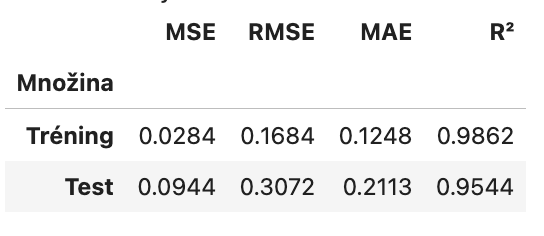
\includegraphics[width=0.37\linewidth,keepaspectratio]{neuronova_siet_metriky_tabulka.png}\hfill
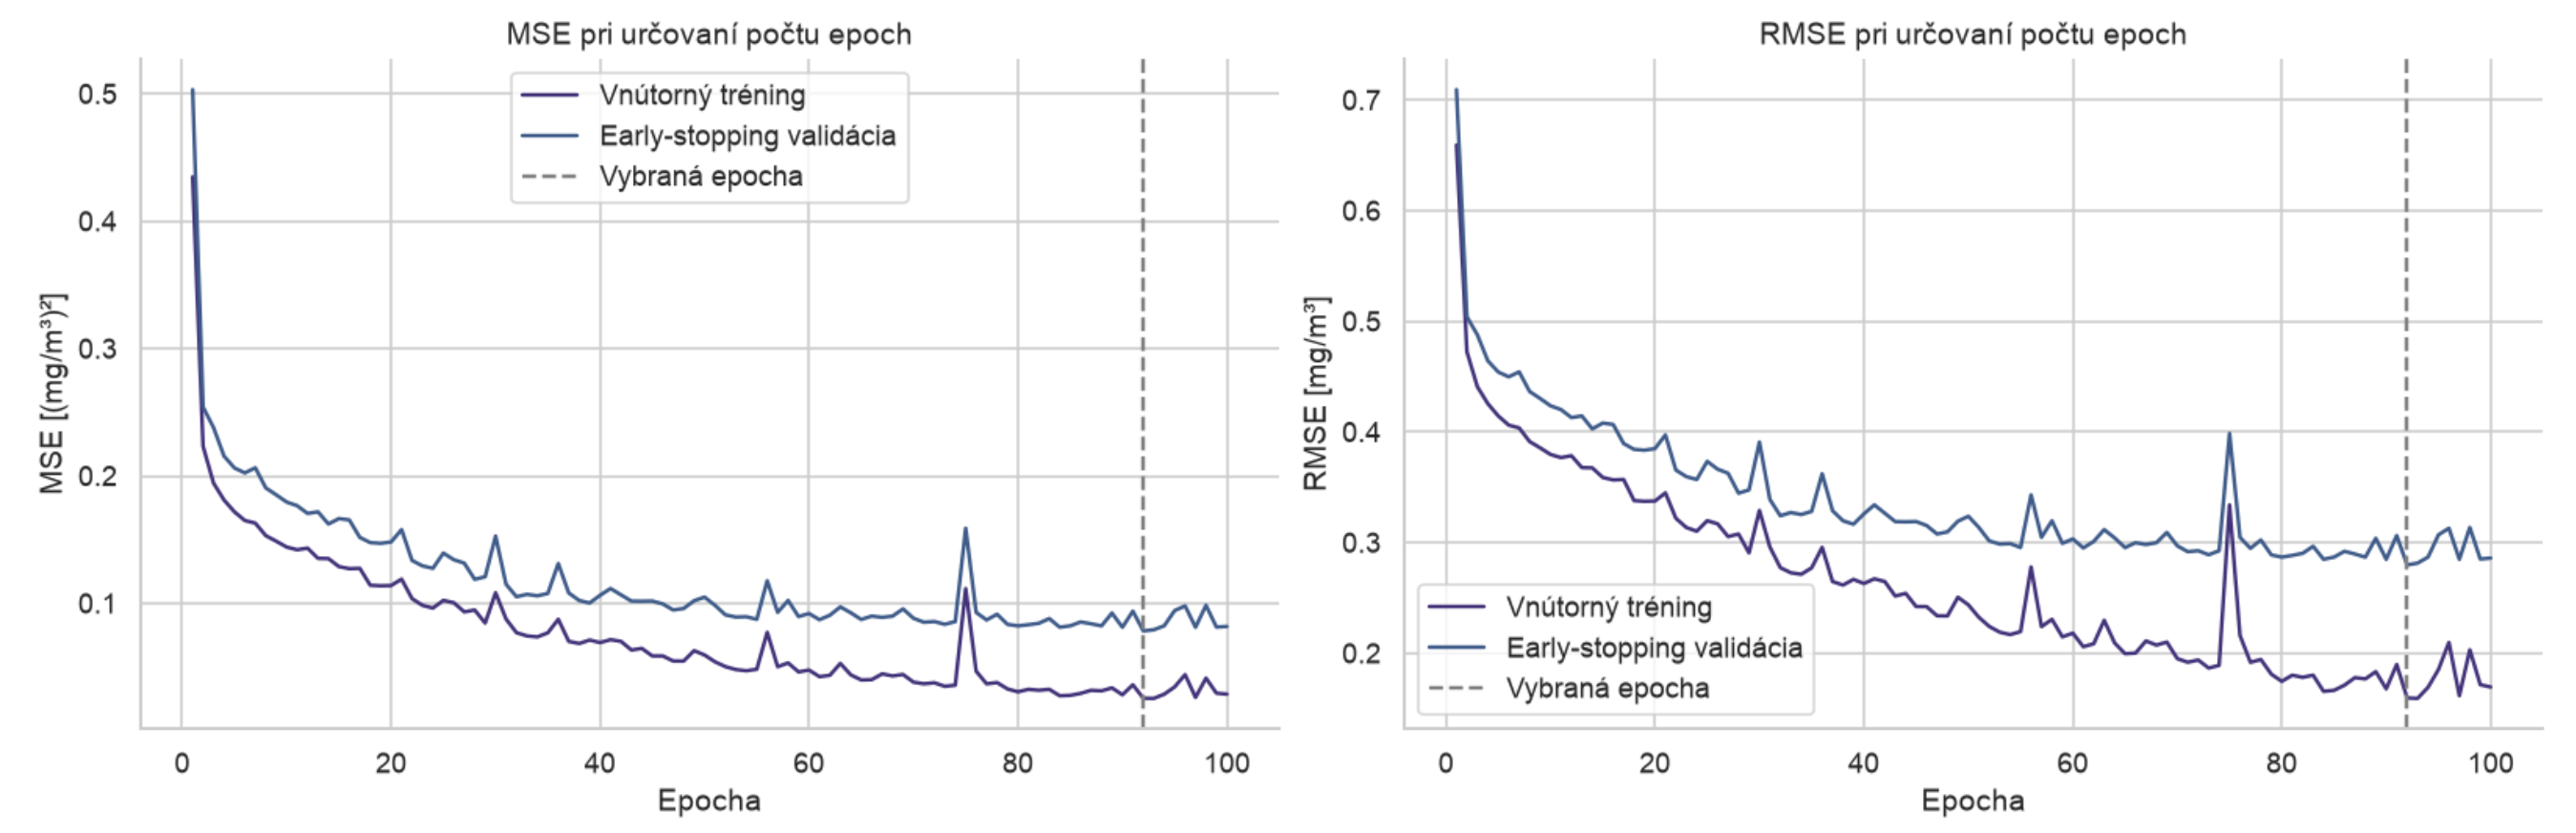
\includegraphics[width=0.60\linewidth,keepaspectratio]{neuronova_siet_krivky_ucenia_graf.png}
\end{center}

% main.ipynb: bunka 189
Early stopping vybral \textbf{92. epochu} z 100 vykonaných. V nej bola vnútorná tréningová MSE 0.0255 a validačná MSE 0.0783. Finálna sieť sa potom učila od začiatku na všetkých tréningových inlieroch. Jej testovacie metriky preto nemusia zodpovedať minimu tejto vnútornej krivky.

\begin{center}
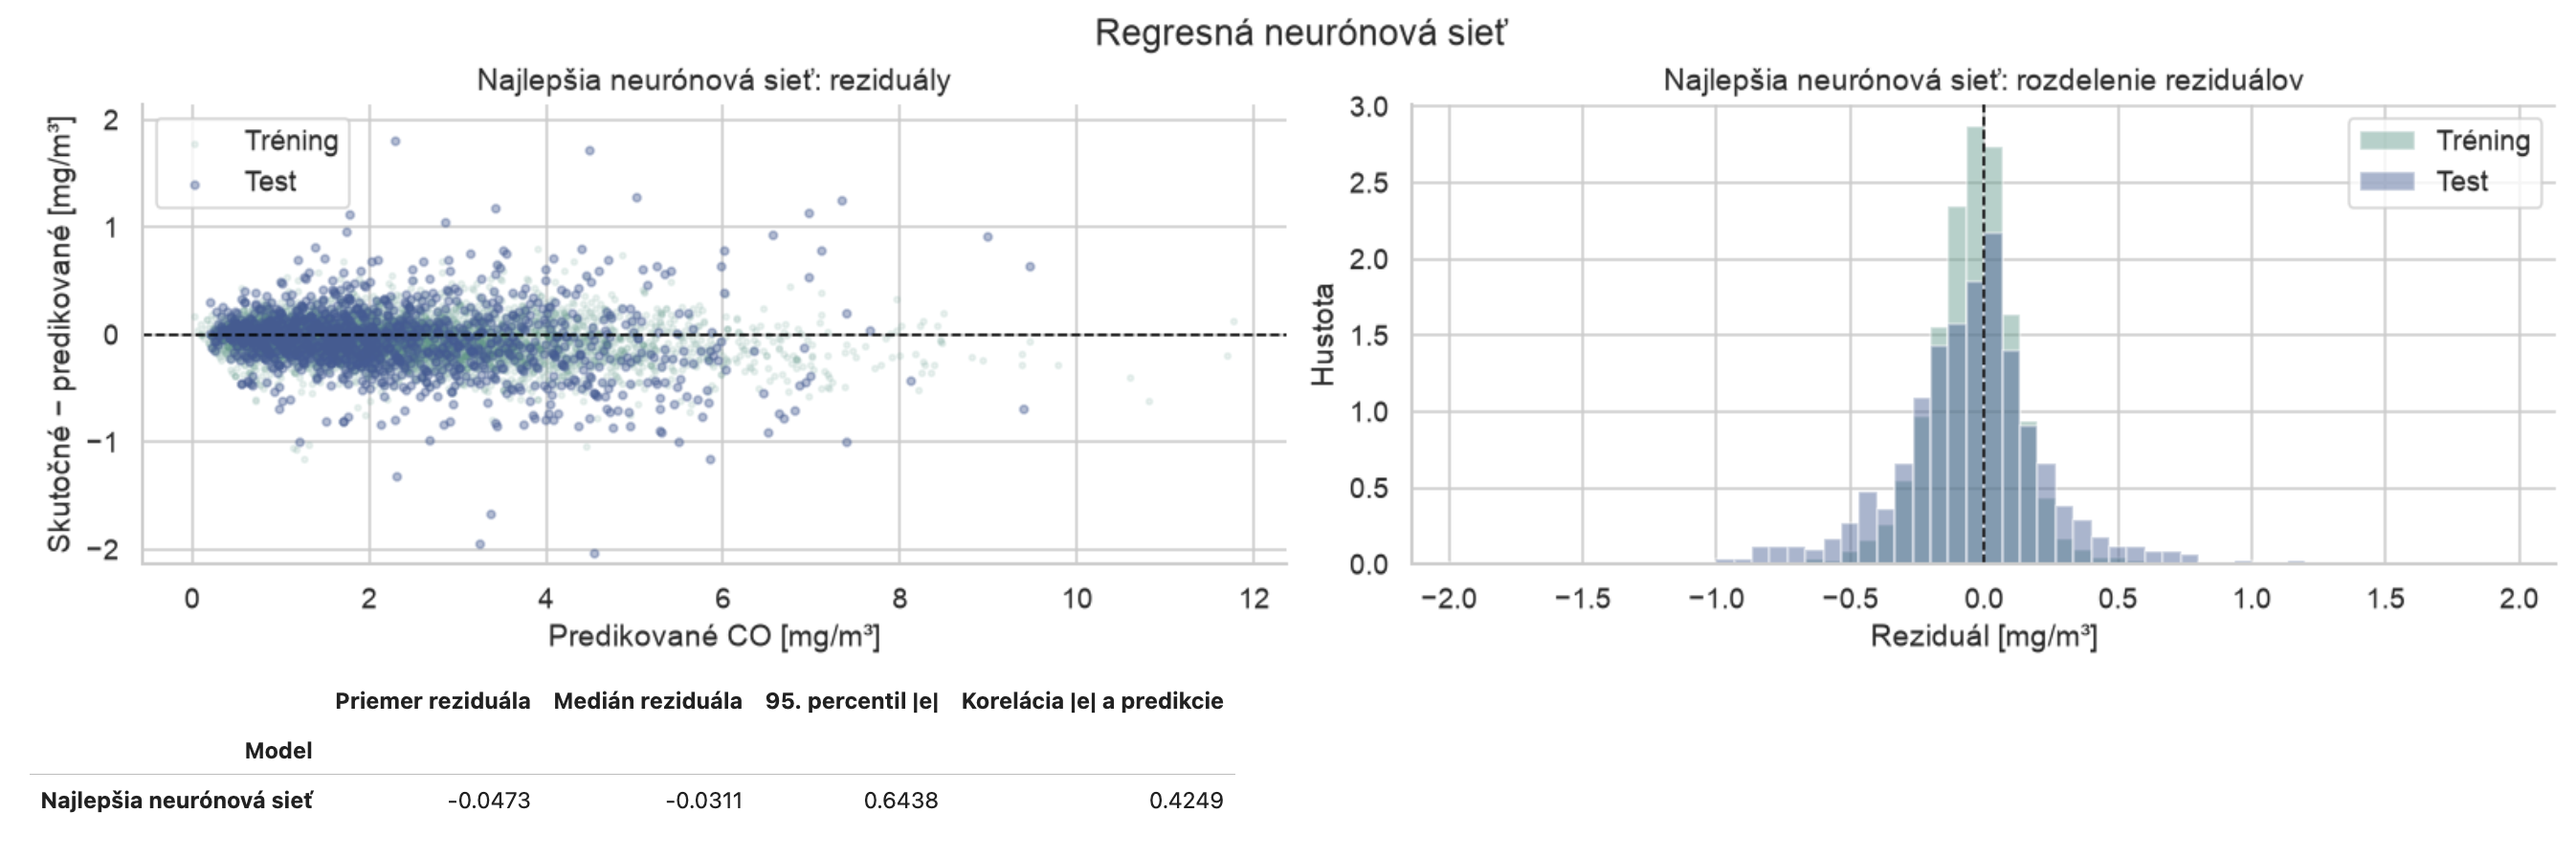
\includegraphics[width=\linewidth,keepaspectratio]{neuronova_siet_rezidualy.png}
\end{center}

% main.ipynb: bunka 191
\textbf{Najlepšia neurónová sieť:} priemerný testovací reziduál -0.0473 \(\mathrm{mg}/\mathrm{m}^3\) znamená nadhodnotenie v priemere. 95 \% absolútnych chýb neprekračuje \textbf{0.644 \(\mathrm{mg}/\mathrm{m}^3\)}. Korelácia veľkosti chyby s predikciou je 0.425. Chyby majú tendenciu rásť s predikovanou koncentráciou.

% main.ipynb: bunka 201
Neurónová sieť a SVR majú na tomto teste veľmi blízku RMSE.
\end{document}
